\mbox{}\\
\vspace{8cm}

This chapter is a reproduction of the following article:

R. Mamede, P. Vila-Cerqueira, J. A. Carriço, M. Ramirez. chewBBACA 3: lowering the barrier for scalable and detailed whole- and core-genome multilocus sequence typing. (2025)


% N. Couto, L. Schuele, E.C. Raangs, M. P. Machado, C. I. Mendes, T. F. Jesus, M. Chlebowicz,  S. Rosema, M. Ramirez, J. A. Carriço, I. B. Autenrieth, A. W. Friedrich, S. Peter and J. W. Rossen. Critical steps in clinical shotgun metagenomics for the concomitant detection and typing of microbial pathogens. Sci Rep 8, 13767 (2018). DOI: \url{https://doi.org/10.1038/s41598-018-31873-w}

The supplementary information referred to throughout the text can be consulted in this chapter before the References section. 

As mentioned in Chapter \ref{ch:introduction}, section \ref{sssec:_intro_shotgun_metagenomics}, \ac{SMg} approaches have been a growing interest to deliver clinically relevant results without \textit{a priori} knowledge of what to expect from a particular clinical sample or patient. 
The capacity to detect all potential pathogens in a sample has great potential utility in the diagnosis of infectious disease. 
However, it is unclear how the variety of available methods impacts the end results.

In this publication, \ac{SMg} was applied to nine body fluid samples and one tissue sample from patients at the University Medical Center Groningen with varying degrees of contamination: one sample from peritoneal fluid, five from pus, two from synovial fluid of knees with a prosthesis, one from sputum and one from a bone biopsy. The results of microbial identification through whole genome sequencing (\ac{WGS}) and \ac{SMg} were compared to standard culture-based microbiological methods. 
In order to evaluate and compare the accuracy and reliability of the bioinformatics analyses in providing the closest results to culture and \ac{WGS} of any cultured isolates, three different bioinformatic pipelines (two commercially and one freely available) were used. Most pathogens identified by culture were also identified through metagenomics, but substantial differences were noted between the taxonomic classification tools. 

My contribution to this publication included the bioinformatics analysis of all the samples using a Unix-based approach. I performed quality assessment and quality control of the \ac{WGS} and \ac{SMg} data, the removal of host sequencing from the samples, and the taxonomic identification of the remaining reads in each sample through 3 different methods: MetaPhlan2, Kraken and MIDAS. Gene detection directly from the reads for bacterial typing was also performed using metaMLST, ReMatCh, Bowtie2 and Samtools. Finally, the reads were assembled using the SPAdes genome assembler, with and without metagenomic mode according to the sample being processed. 

\cleardoublepage 

\begin{center}
\large
\textbf{chewBBACA 3: lowering the barrier for scalable and detailed whole- and core-genome multilocus sequence typing}
\end{center}

Rafael Mamede$^{1,2}$, 
Pedro Vila-Cerqueira$^{1}$,
João André Carriço$^{1}$,
Mário Ramirez$^{1}$

$^1$ Instituto de Microbiologia, Instituto de Medicina Molecular, Faculdade de Medicina, Universidade de Lisboa, Portugal;

$^2$ Gulbenkian Institute for Molecular Medicine.

\section{Abstract} \label{sec:ch2_abstract}

\subsection{Background} \label{ssec:ch2_abstract}

The wide adoption of whole genome sequencing has enabled the implementation of genomics-based systems, which provide unparalleled resolution for the surveillance and outbreak investigation of bacterial pathogens. To fully exploit the wealth and complexity of genomics data, bioinformatics methods need to be highly scalable, provide accurate and extensive data for potential downstream analyses, as well as analytic capabilities. Here, we present chewBBACA 3, a suite of modules for scalable and comprehensive bacterial whole- and core-genome multilocus sequence typing (wg/cgMLST) with built-in features to create new schemas, evaluate loci diversity and strain similarity.

\subsection{Results} \label{ssec:ch2_abstract}

chewBBACA 3 enables faster and more accurate schema creation and allele calling by complementing an alignment-based approach with alignment-free methods, including hash-based comparisons and minimizer-based clustering. Schema creation is up to 55-fold faster and identifies up to 10\% more loci than its predecessor, chewBBACA 2. Furthermore, chewBBACA 3 can quickly adapt or import schemas available on external wg/cgMLST platforms or Chewie-NS, promoting interoperability. The efficiency of allele calling allows processing larger genome collections, from thousands to tens of thousands of genomes, at the whole- and core-genome levels without requiring high computational resources and being up to 52-fold faster than similar tools. chewBBACA 3’s enhanced sensitivity allows it to identify and classify more schema loci and coding sequences than the compared methods, resulting in higher resolution for strain comparison. Moreover, the allelic profiles, classification statistics and associated sequence data produced by chewBBACA 3 can be the basis for detailed analyses that provide added value in surveillance and outbreak investigation settings. New modules leverage the potential of the schema and allele call results data to create interactive reports that enable an intuitive and in-depth analysis of allele diversity in loci of interest and allow assessing strain similarity based on loci presence, allelic distances and phylogenetic analysis.

\subsection{Conclusions} \label{ssec:ch2_abstract}

chewBBACA 3 provides functionalities for complete wg/cgMLST analysis at scale, lowering the barrier for the use of wg/cgMLST and offering extensive results and analytic capabilities for streamlined, comprehensive, and local analyses. chewBBACA 3 is freely available at \url{https://github.com/B-UMMI/chewBBACA}.

\section{Background} \label{sec:ch2_background}

The burden of bacterial infections constitutes a major challenge to public health systems worldwide \citep{ikuta_global_2022, noauthor_who_2024}. The advances in sequencing technologies have enabled public health institutions to support and gradually transition to whole genome sequencing (WGS), increasing surveillance capacity and the effectiveness of outbreak investigations. WGS offers high-resolution discrimination of closely related bacterial strains and enables the identification of pathogens’ relevant features in a timely and accurate manner, aiding in reaching an informed decision for effective disease prevention and control \citep{authority_efsa_efsa_2024, struelens_real-time_2024, european_centre_for_disease_prevention_and_control_ecdc_2019, authority_efsa_guidelines_2022}. The widespread use of WGS, as well as the adherence to FAIR principles, encouraged the development of efficient bioinformatics methods for in silico multilocus sequence typing (MLST), serotyping, and the identification of antimicrobial resistance and virulence determinants. It also allowed transitioning to methods with enhanced resolution that leverage the full genomic content to identify relevant features and provide a more accurate measure of strain similarity \citep{uelze_typing_2020}.

These methods are diverse but generally adopt one of three fundamental approaches: i) determining Single-Nucleotide Variants (SNVs) relative to a reference genome, ii) measuring sequence similarity based on short subsequences of length k, known as k-mers, and iii) comparing the strains' gene content, referred to as gene-by-gene methods (GbG) \citep{uelze_typing_2020}.

SNV approaches detect differences at the single nucleotide level by mapping sequencing reads against a closely related reference strain. The precision level of this approach enables the identification of point mutations or more complex variants that can be determinants of phenotypic characteristics of interest, such as increased virulence and antimicrobial resistance. The choice of the reference genome is crucial as the quality and relatedness of the reference genome to the strains of interest can greatly influence the number of shared positions compared and, therefore, the extent of the variability detected \citep{bush_genomic_2020, valiente-mullor_one_2021}. k-mer-based tools split genomic sequences into k-mers and compare the resulting k-mer sets to estimate strain similarity or identify regions of interest. These approaches can estimate similarity without needing a reference genome and are potentially faster and more computationally efficient than SNV or GbG approaches. The efficiency of these approaches depends on the sampling method used to select k-mers, which should be fine-tuned to achieve a good balance between efficiency and accuracy for the desired application \citep{ndiaye_when_2024, belbasi_minimizer_2022}. With the wide adoption of WGS, GbG approaches have transitioned from classical MLST to whole-genome and core-genome MLST (wg/cgMLST). wg/cgMLST enables the creation of schemas encompassing the variability of hundreds to thousands of loci for a species of interest to accurately determine the loci and alleles present in strains of interest. Creating and maintaining wg/cgMLST schemas to capture a species' diversity is crucial for the accuracy of GbG methods and can be a laborious process. As with SNV approaches, knowing the alleles present at a given locus can be linked to phenotypic properties such as virulence or antimicrobial resistance.

It has been shown that applying any of these approaches can generate results suitable for accurate strain similarity estimation and phylogenetic analyses in surveillance and outbreak scenarios \citep{uelze_typing_2020, bush_genomic_2020, valiente-mullor_one_2021, ndiaye_when_2024, belbasi_minimizer_2022, king_comparison_2024}. Nevertheless, wg/cgMLST has been more frequently integrated into surveillance and outbreak detection systems, partly due to constituting an expansion of classical MLST, which conceptually and technically allows for a more straightforward implementation, specially in constantly growing datasets such as the ones used in long-term epidemiological surveillance. The capacity to update wg/cgMLST schemas with new alleles increases the diversity captured by and, consequently, the resolution of wg/cgMLST analyses. Moreover, wg/cgMLST allows establishing allelic nomenclatures for standardised comparisons. Existing solutions for wg/cgMLST analysis can vary greatly in the degree of data centralisation, analytical capabilities, and license type \citep{jolley_bigsdb_2010, zhou_enterobase_2020, mamede_chewie_2021}. To continue to promote the adoption of wg/cgMLST, improvements should focus on interoperability to facilitate comparison of results, scalability to meet growing data processing demands, and easily performed comprehensive local analyses to offer powerful analytic capabilities to end users while complying with strict data privacy laws.

To provide a solution for scalable, detailed, and local wg/cgMLST, we developed chewBBACA 3, which vastly improves and extends the functionalities of chewBBACA 2 \citep{mamede_chewie_2021, silva_chewbbaca_2018}, a widely used tool for wg/cgMLST which has been integrated into public health workflows such as EFSA's One Health WGS system, used for rapid detection of multi-country foodborne outbreaks in collaboration with the European Centre for Disease Prevention and Control (ECDC) \citep{authority_efsa_guidelines_2022}.

\section{Implementation} \label{sec:implementation}

\subsection{Overview} \label{ssec:overview}

chewBBACA 3 is a complete reimplementation of its predecessor, chewBBACA 2 \citep{mamede_chewie_2021}, which was already an upgraded version of chewBBACA’s first published version \citep{silva_chewbbaca_2018}. chewBBACA 3 provides a modular approach for complete wg/cgMLST analysis allowing more efficient and accurate schema creation and allele calling and offering interactive reports for comprehensive schema and results analyses \ref{fig:chap2_figure1A}. chewBBACA 3 allows to set up schemas for wg/cgMLST through the use of larger collections of genome assemblies or coding DNA sequences (CDSs) in FASTA format or by adapting existing schemas from external platforms \citep{jolley_bigsdb_2010, zhou_enterobase_2020, noauthor_cgmlstorg_nodate}. Additionally, the integration with Chewie-NS, which was previously described together with chewBBACA 2 \citep{mamede_chewie_2021}, allows easily importing ready-to-use schemas to obtain comparable interlaboratory results based on a common allelic nomenclature. To determine the allelic profiles of strains of interest, chewBBACA 3 identifies and clusters the distinct CDSs predicted from the strains' genomes, significantly reducing the number of comparisons against the schema loci in contrast to the sequential strain processing used by chewBBACA 2. This translates into faster and more efficient allele calling and facilitates data aggregation to create output files with more detailed results. Allele calling identifies and adds new alleles to schemas, ensuring that they are gradually updated to produce accurate and comparable results over time. Similarly to chewBBACA 2, new alleles are inferred based on the BLAST Score Ratio (BSR) \citep{rasko_visualization_2005} computed from BLASTp alignments \citep{camacho_blast_2009}, complying with minimum sequence length and allele size variation thresholds \citep{silva_chewbbaca_2018}. Adjustments to these parameters allow chewBBACA 3 to classify more CDSs and capture loci diversity more accurately. chewBBACA 3 increases the granularity of the results by expanding the set of special classifications assigned when the presence of a locus cannot be inferred confidently, such as when a CDS matching a schema locus is outside the user-specified locus size variation interval or if multiple CDSs from a genome match the same schema locus \ref{fig:chap2_figureS1, fig:chap2_figureS2, fig:chap2_figureS3, fig:chap2_figureS4}(Figures S1-S4, Additional File 1). These special classifications aid in identifying spurious alleles resulting from low-quality data, pseudogenes, and paralogous loci. The set of core loci can be determined based on the allele calling results for any locus presence threshold, and the resulting list of core loci can be used to perform allele calling at the core genome level. Schema loci can be annotated by searching for matches through UniProt’s SPARQL endpoint, which was already an option in chewBBACA 2, and now also by aligning a schema’s alleles against UniProt’s reference proteomes to retrieve annotations based on higher-quality entries \citep{the_uniprot_consortium_uniprot_2025}. New schema and results evaluation modules leverage the power of the React JavaScript library \citep{noauthor_react_nodate} to build interactive reports that enable local and comprehensive analyses of the diversity of loci contained in schemas and aid in identifying closely related strains for more effective surveillance and outbreak assessment.

\subsection{Core modules} \label{ssec:core_modules}

While all the modules in chewBBACA 2 were reimplemented to increase the scalability and comprehensiveness of the results generated by chewBBACA 3, module development concentrated primarily on the CreateSchema and AlleleCall modules (Figures S5 and S6, Additional File 1), which handle schema creation and allele calling, respectively. Gene prediction was optimised in both modules using Pyrodigal \citep{larralde_pyrodigal_2022, hyatt_prodigal_2010}, a Python module that provides bindings to Prodigal for seamless integration and offers several advantages, such as faster gene prediction and greater control over gene prediction parameters and results. Additionally, a novel feature was added allowing both modules to accept FASTA files with CDSs, enabling users to leverage the vast CDS data available in public databases or provide CDSs predicted by other gene prediction tools if preferred by the user, such as GeneMarkS-2 or Balrog \citep{lomsadze_modeling_2018, sommer_balrog_2021}. Following the gene prediction step, CDS deduplication is performed at both DNA and protein levels to identify the set of distinct CDSs. The distinct translated CDSs are clustered based on the proportion of shared minimizers ($\geq0.2$) with representative alleles \citep{schleimer_winnowing_nodate, roberts_reducing_2004, marcais_improving_2017} (Figure 1B:1-3). The minimizer parameters (k=5, w=5, lexicographic order) were chosen to select sets of k-mers that would cover most sequence positions at least once while also keeping memory usage low \citep{zheng_improved_2020}. The low clustering threshold groups similar sequences into the same clusters, reducing the number of comparisons in subsequent steps. For schema creation, the CDSs sharing a high proportion of minimizers ($\geq0.9$) with the cluster representative or larger CDSs are considered alleles of the same locus and are excluded (Figure 1B:4). The clustering results are complemented by intracluster and intercluster alignment with BLASTp to exclude CDSs based on the BSR threshold and select the final set of CDSs (Figure 1B:5). This defines the schema by creating a schema seed with one representative allele for each locus. This schema seed will be used by the AlleleCall module, which may add further representative alleles to capture the allelic diversity at each locus. The AlleleCall module uses the same functions as the schema creation process for sequence deduplication and CDS clustering. Another novel feature implemented is that each distinct CDS is hashed, mapped to the compressed list of genomes that contain it (Figure S7, Additional File 1) and compared against the hashed schema alleles. This allows keeping the information about the CDSs identified in all strains in memory, enabling fast exact matching and classification of all genomes containing a CDS based on a single match. Clustering and intracluster alignment with BLASTp allow comparison of the remaining unclassified CDSs against the schema's representative alleles to find and classify inexact matches (Figure 1B:1-4). A final step aligns the schema's representative alleles against the remaining unclassified CDSs to find more divergent alleles and select new representative alleles (Figure 1B:5). The matches found throughout the process are evaluated at the end of the process to assign the final classifications, create the allelic profiles, and update the schema with novel alleles. Both core modules create several output files with detailed schema and results data that support the analyses performed by other modules and can serve as the basis for custom analyses that seek to answer relevant questions at the strain or population-wide level.
A more detailed description of the implementation and functionalities included in each module is available in the supplementary material (Additional File 1) and in chewBBACA’s online documentation \citep{noauthor_chewbbaca_nodate}.

\begin{figure*}[h!]
    \centering
    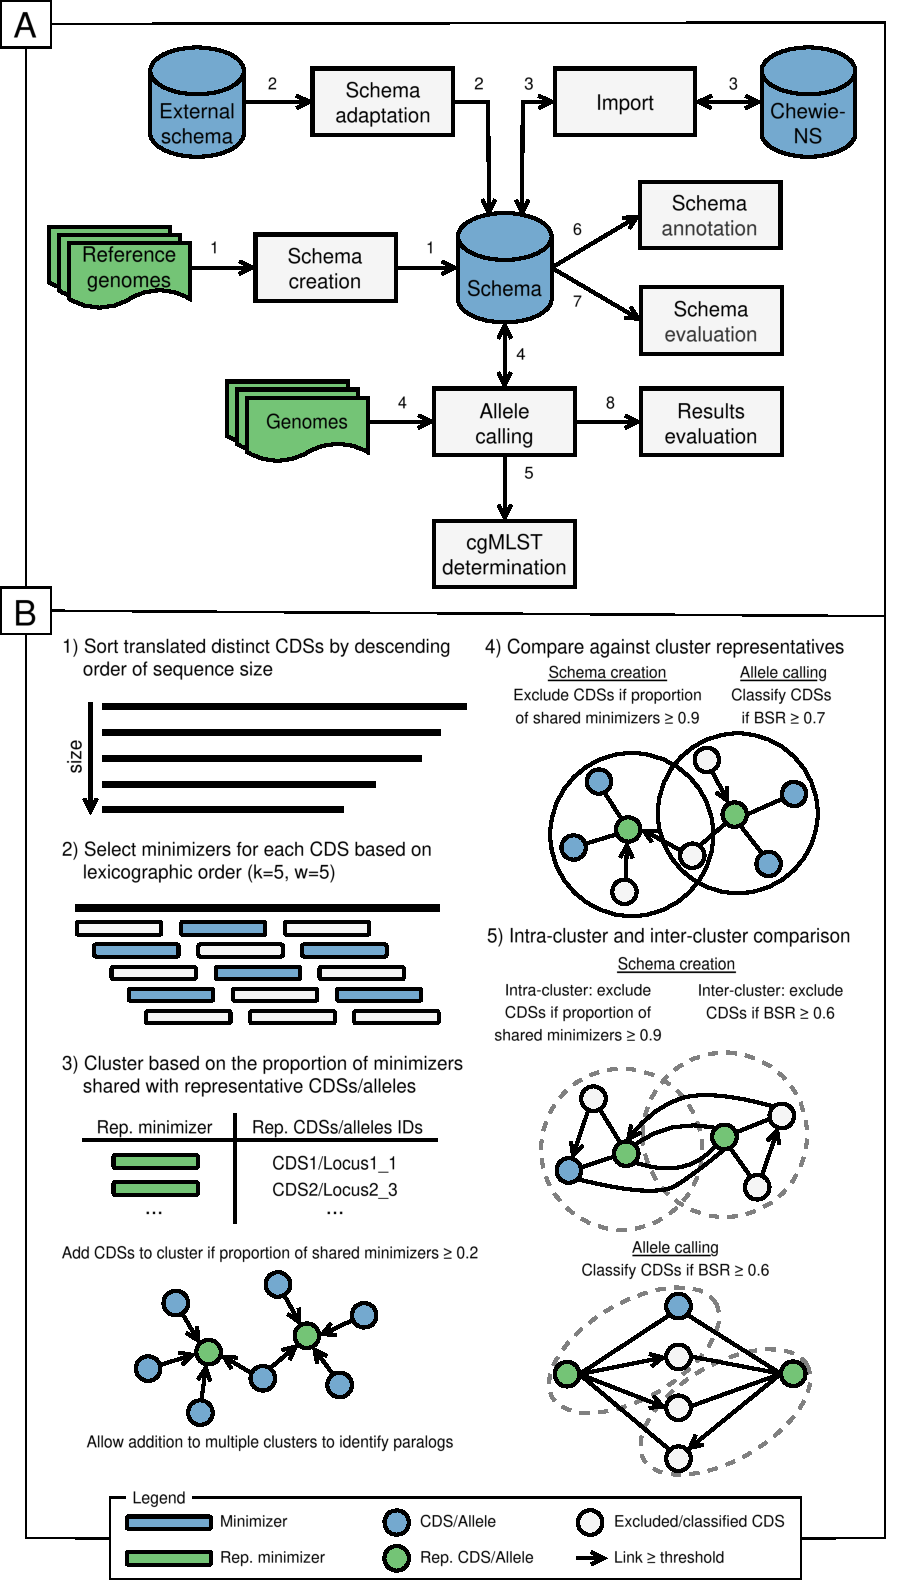
\includegraphics[angle=0,height=0.92\textheight]{figures/chapter 2/Figure1.pdf}
    \label{fig:chap2_figure1}
\end{figure*}
\vspace*{-6mm}
\begin{center}
    \emph{(Caption on next page.)}
\end{center}
\begin{figure*}[h!]
    \caption{Overview of chewBBACA 3’s processes and minimizer-based clustering used by the \textit{CreateSchema} and \textit{AlleleCall} modules. (A) chewBBACA 3 includes modules for schema setup (steps labeled with 1, 2 and 3), allele calling (steps labeled with 4), core genome determination (steps labeled with 5), schema annotation (steps labeled with 6), schema evaluation (steps labeled with 7), and results evaluation (steps labeled with 8). Blue cylinder icons represent schemas, with the central cylinder icon representing a schema created or adapted for usage with chewBBACA 3. Green document icons represent input FASTA files. Grey rectangle icons represent analysis processes available in chewBBACA 3. (B) Minimizer-based clustering and classification steps implemented in the \textit{CreateSchema} and \textit{AlleleCall} modules. (Step 1) The distinct translated CDSs not classified through exact matching at the DNA and protein levels are sorted based on decreasing size. (Step 2) Minimizers are selected from the set of 5-mers for each CDS based on lexicographic order and a window size of 5. (Step 3) The set of minimizers selected for each CDS is compared against the minimizers of CDSs selected as cluster representatives (\textit{CreateSchema}) or the schema loci representative alleles (\textit{AlleleCall}) to cluster CDSs based on a proportion of shared minimizers $\geq0.2$. (Step 4) The CDSs that share a proportion of minimizers $\geq0.9$ (\textit{CreateSchema}) or a BSR $\geq0.7$ (AlleleCall) with the cluster representative are excluded from the analysis (\textit{CreateSchema}) or classified (\textit{AlleleCall}). (Step 5) Non-representative CDSs from the same cluster are compared to exclude smaller CDSs that share a proportion of minimizers $\geq0.9$ with larger CDSs (CreateSchema). Representative CDSs or alleles are aligned against all CDSs to exclude (\textit{CreateSchema}) or classify (\textit{AlleleCall}) CDSs based on a default BSR value of 0.6.}
\end{figure*}


% (Table \ref{tab:ch2_table_1}).
% \ref{fig:chap2_figure1A}
% \begin{landscape}
% \begin{table}[]
\caption{Characteristics of the samples and mapping of trimmed reads against a human genome hg19 (\%) using CLC Genomics Workbench v10.0.1.}
\label{tab:ch2_table_1}
\resizebox{\linewidth}{!}{%
\small
\begin{tabular}{@{}llllll@{}}
\toprule
\textbf{Sample} & \textbf{Sample type} & \textbf{DNA extraction method} & \textbf{Total number of reads} & \textbf{Mapped reads against hg19} & \textbf{Unmapped reads} \\ \midrule
Sample 1         & Peritoneal fluid & Ultra-Deep Microbiome Prep (Molzym) & 5892978 & 5,249,063 (89.2\%) & 632,951 (10.8\%)   \\
Sample 2         & Pus (abscess)    & Ultra-Deep Microbiome Prep (Molzym) & 9603346 & 7,828.746 (81.6\%) & 1,770,558 (18.4\%) \\
Sample 3         & Synovial fluid   & Ultra-Deep Microbiome Prep (Molzym) & 8615810 & 8,254,594 (95.9\%) & 355,200 (4.1\%)    \\
Sample 4         & Synovial fluid   & Ultra-Deep Microbiome Prep (Molzym) & 6078166 & 6,015,945 (99.0\%) & 61,099 (1.0\%)     \\
Sample 5         & Pus (abscess)    & Ultra-Deep Microbiome Prep (Molzym) & 8368930 & 309,588 (3.7\%)    & 8,052,272 (96.3\%) \\
Sample 6         & Pus (empyema)    & QIAamp DNA Microbiome Kit (Qiagen)  & 2912802 & 2,877,066 (98.8\%) & 34,506 (1.1\%)     \\
Sample 7         & Pus (empyema)    & QIAamp DNA Microbiome Kit (Qiagen)  & 1486700 & 922,932 (62.2\%)   & 561,772 (37.8\%)   \\
Sample 8         & Bone biopsy      & Micro-DXTM (Molzym)                 & 6534866 & 229,149 (3.5\%)    & 6,303,803 (96.5\%) \\
Sample 9         & Pus (abscess)    & Micro-DXTM (Molzym)                 & 6173132 & 6,081,612 (98.5\%) & 89,922 (1.5\%)     \\
Sample 10        & Sputum           & Micro-DXTM (Molzym)                 & 7596836 & 7,337,832 (96.7\%) & 235,520 (3.3\%)    \\
Negative control & Water            & QIAamp DNA Microbiome Kit (Qiagen)  & 1730738 & 1,706,861 (98.9\%) & 19,805 (1.2\%)     \\ \bottomrule
\end{tabular}%
}
\end{table}
% \end{landscape}

%0.2 ng/$\mu$l and 1 ng
%\ref{tab:ch2_table_1})

% Reference scronyms
%\ac{WGS}
%All the parameters used in each approach are available in Supplementary Table 1 (see \ref{ch2_supmaterial}).

\section{Results and discussion} \label{sec:results_and_discussion}

\subsection{Fast wg/cgMLST schema creation or retrieval from multiple sources} \label{ssec:results_discussion_ssec1}

chewBBACA 3 offers three options for setting up a schema for wg/cgMLST analysis.

The first option is creating a new schema by selecting loci from a set of complete or draft genome assemblies with the CreateSchema module to create a schema seed (Figure S5, Additional File 1). To evaluate the performance of the CreateSchema module, we created schema seeds with chewBBACA 3 and chewBBACA 2 based on the complete genome assemblies available on the NCBI RefSeq database \citep{sayers_database_2022} for three bacterial species: Streptococcus pyogenes (n=260), Listeria monocytogenes (n=309), and Salmonella enterica (n=1,326). Schema seed creation was 25- to 55-fold faster with chewBBACA 3 than with chewBBACA 2, with similar memory usage (Table S1, Additional File 2). A comparison of the schema seeds generated with both versions revealed that the schema seeds created by chewBBACA 3 contained 98\% of the loci identified by chewBBACA 2 (Table S2, Additional File 2). Moreover, chewBBACA 3 identified 6\% to 10\% more loci than chewBBACA 2, primarily due to a more accurate identification of smaller loci. Ideally, target loci should be defined based on a set of high-quality genome assemblies to avoid the inclusion of spurious loci in the schema seed. Nonetheless, schema seed creation with chewBBACA 3 will remain efficient even when using larger genome collections, possibly including draft genomes, to adequately capture a species diversity.

A second option is to adapt schemas from external platforms with the PrepExternalSchema module (Figure S8, Additional File 1). This module filters out incomplete alleles (i.e. alleles that contain ambiguous bases or not corresponding to valid CDSs, such as having no start/stop codon) and selects representative alleles based on a BSR threshold to create a schema structure compatible with chewBBACA. Schema adaptation promotes the usage of schemas previously made available and adopted by the community, contributing to the integration and interoperability with other platforms. chewBBACA 3 is over three orders of magnitude faster than chewBBACA 2 when adapting the cgMLST schemas for S. pyogenes, L. monocytogenes, and S. enterica available on the cgMLST.org server \citep{noauthor_cgmlstorg_nodate}, adapting any of the schemas in under five minutes (Table S3, Additional File 2). Furthermore, contrarily to chewBBACA 2, chewBBACA 3 now ensures that the selected representative alleles fully capture the diversity of each locus based on the specified BSR threshold (Table S4, Additional File 2). chewBBACA 3 also provides options to filter out alleles based on user-defined sequence size and size variation thresholds and outputs detailed information about the changes made while adapting a schema to inform the user of the changes introduced to the existing schema.

Lastly, the third option is the DownloadSchema module (Figure S9, Additional File 1), one of the modules (Figures S9-S11, Additional File 1) developed to integrate with Chewie-NS \citep{mamede_chewie_2021} [15], allowing users to import ready-to-use schemas from Chewie-NS instances. This option offers the advantage of enabling local and private analysis based on a common allelic nomenclature to facilitate the comparison of results. Schemas downloaded from Chewie-NS can be kept up-to-date by synchronizing with the remote versions to receive the latest allele data submitted by other users and, if desired, contribute novel alleles identified locally.

\subsection{Scalable and efficient allele calling} \label{ssec:results_discussion_ssec2}

We performed allele calling with the schema seeds created with chewBBACA 3 in the previous section and the complete genomes for each species to add new alleles to the schemas and determine the set of core loci with the ExtractCgMLST module (Figure S12, Additional File 1). The lists of core loci (present in 100\% of the genomes) were used to measure performance at the cgMLST level for datasets including between 1 and 16,384 draft genome assemblies and compared against the results obtained with chewBBACA 2 and pyMLST \citep{biguenet_introduction_2023} for equivalent schemas and databases (Table S5, Additional File 2). chewBBACA 3 processed all datasets faster than chewBBACA 2 and pyMLST. On average, chewBBACA 3 was 1.9- to 20.3-fold and 1.3- to 51.9-fold faster than chewBBACA 2 and pyMLST, respectively (Figure 2A and Table S6, Additional File 2). The difference increased with dataset size, largely due to the increased redundancy (same sequence found in different genomes) of the set of CDSs extracted from the genomes (Table S7, Additional File 2). For example, only 1.5\% to 2.8\% of the total CDSs identified in the complete datasets (n=16,384) were distinct. By identifying the set of distinct CDSs before trying to match them against the schema loci, chewBBACA 3 avoids the repeated evaluation of identical CDSs identified in multiple genomes.

\begin{figure*}[h!]
    \centering
    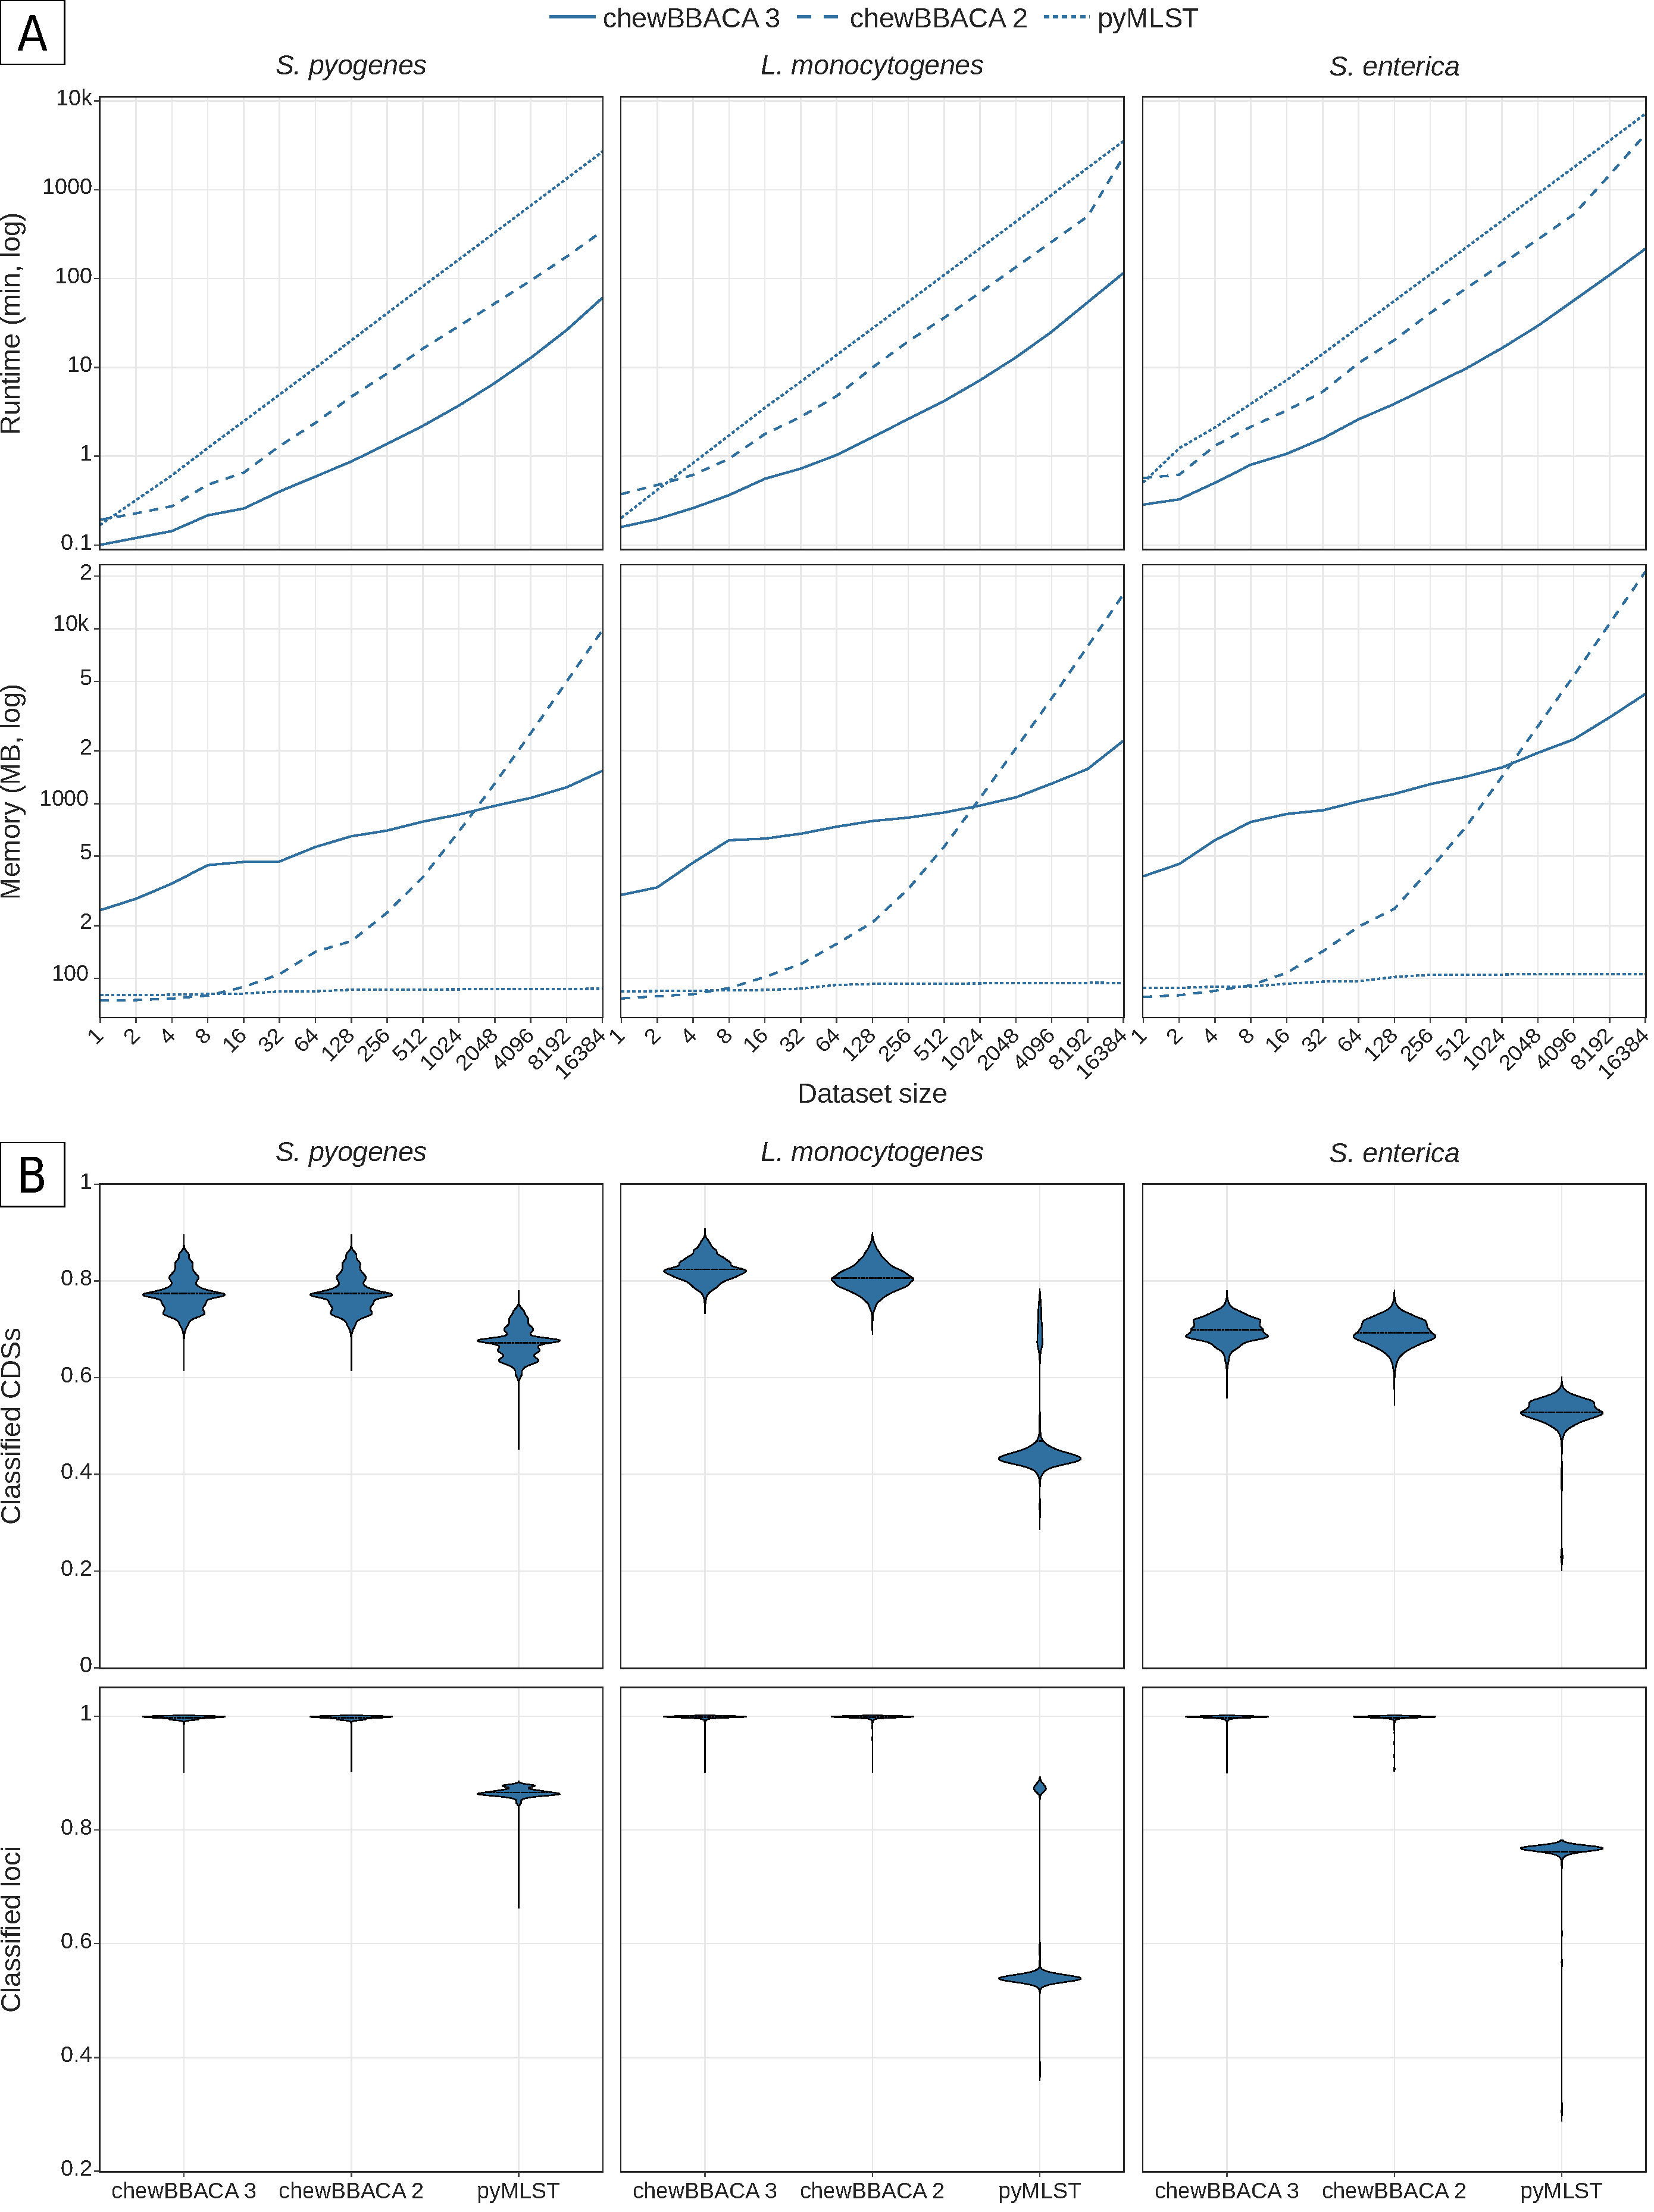
\includegraphics[angle=0,width=0.93\textwidth]{figures/chapter 2/Figure2.pdf}
    \caption{Performance comparison of chewBBACA 3, chewBBACA 2 and pyMLST. (A) Runtime and peak memory usage comparison for the allele calling of datasets with a varying number of genomes (from 1 to 16,384) for three bacterial species: Streptococcus pyogenes, Listeria monocytogenes, and Salmonella enterica. The benchmark was performed with five replicates per dataset size, except for the complete dataset (n=16384). The values shown are the mean of the replicate values for each dataset. Runtime was measured as the elapsed real time in minutes (logarithmic scale). Peak memory usage was measured as the maximum resident set size in MB (logarithmic scale). (B) Proportion of strain CDSs and schema loci classified for the complete datasets (n=16384). The proportion of classified CDSs corresponds to the number of CDSs classified by each tool divided by the total number of CDSs predicted for each strain by Pyrodigal. The proportion of classified loci corresponds to the number of schema loci identified by each tool divided by the total number of schema loci.}
    \label{fig:chap2_figure2}
\end{figure*}

Additionally, the novel minimizer-based clustering matches the remaining CDSs to the most similar schema loci, reducing comparisons between dissimilar sequences. These two steps contribute the most to the increased speed compared to chewBBACA 2 and pyMLST, which process each genome separately and additionally do not take advantage of multiprocessing settings as efficiently as chewBBACA 3. Regarding peak memory usage (Figure 2A and Table S8, Additional File 2), chewBBACA 3 used, on average, 8.6- to 1.1-fold more memory than chewBBACA 2 for datasets with up to 1,024 strains. The inverse was observed for larger datasets, with chewBBACA 2 using 1.1- to 6.9-fold more memory than chewBBACA 3. Compared to pyMLST, chewBBACA 3 used 3.1- to 40-fold more memory. pyMLST maintains low memory usage irrespective of dataset size but is single-threaded and only supports the addition of one strain per command, which limits its scalability. chewBBACA 3 enables considerably faster analyses while keeping memory usage in check to allow large-scale analysis without needing high-performance computing infrastructures. While comparing results using the entire wgMLST schema would further highlight chewBBACA 3’s efficiency and accuracy, time and memory constraints related to running chewBBACA 2 and pyMLST under the same conditions invalidated such comparison.

The thoroughness of the allele calling in chewBBACA 3 can be controlled through four execution modes (Figure S6, Additional File 1). Mode 1 identifies exact matches at the DNA level between the genomes’ CDSs and the schema alleles. Mode 2 adds exact matching at the protein level, enabling the identification of novel alleles with synonymous substitutions. Mode 3 proceeds to clustering and intracluster alignment to identify similar alleles based on the BSR threshold. Mode 4, the default, runs the complete process to classify as many CDSs as possible and potentially selects new representative alleles, preparing the schema to better identify future novel alleles. Modes 1 and 2 offer a 4.7-fold speedup over the default mode (Figure S13, Additional File 1 and Tables S9 and S10, Additional File 2), but their capacity for allele identification is limited to only modestly divergent alleles. This makes them appropriate for applications where a less accurate but much faster strain discrimination is sufficient, or for faster allele calling with schemas that already capture most of a species’ diversity for the set of loci that make up those schemas, as is the case for many publicly available cgMLST schemas. Mode 3 provides similar accuracy to the default mode in less time, with a more significant reduction in runtime for larger schemas and more diverse datasets. Mode 4 offers greater sensitivity to identify the most divergent alleles and select new representative alleles to add to schemas, which is essential to increase the diversity captured by a schema, especially in the initial phase of schema development. For schemas that already include representative alleles that capture a species diversity, Mode 3 and Mode 4 may only differ in the number of special classifications attributed, with Mode 4 identifying more.

chewBBACA 2 added new alleles to schemas automatically, not providing any option for users to prevent the allele call process from changing an existing schema. chewBBACA 3 includes the --no-inferred option to control this behaviour. This option can be helpful in several scenarios, including: updating schemas only periodically, in applications where frequent schema updates can compromise the reproducibility of the allele calling; classifying genomes from closely related species to identify similar loci; and avoiding adding spurious alleles to a schema when there's uncertainty about the quality level of the genome assemblies being analyzed.

\subsection{Comprehensive allele calling for more accurate and detailed results} \label{ssec:results_discussion_ssec3}

We evaluated the allele calling results for the complete dataset of each of the three species chosen (consisting of 16,384 genomes) to measure the comprehensiveness of chewBBACA 3's results and compare it against chewBBACA 2 and pyMLST. Results were compared at the core and accessory genome levels, based on a locus presence threshold of 95\%, of the cgMLST schemas defined above. Concordance was measured by comparing the pairwise Jaccard distances computed based on the allelic profiles. The core and accessory loci sets determined based on chewBBACA 3’s and chewBBACA 2’s results were highly similar, sharing over 99\% and 95\% of the loci at the core and accessory levels, respectively (Table S11, Additional File 2). The pairwise Jaccard distances were strongly correlated and near the identity line, indicating high concordance between the results (Figure 3), with the pairwise allelic distances computed by both tools differing by 0 to 6 differences on average (Figure S14, Additional File 1). The core loci sets determined based on pyMLST’s results were considerably smaller, containing 42\% to 80\% of the schema loci, compared to over 94\% for chewBBACA 3. The reduced number of core loci identified by pyMLST is related to an inconsistent identification of some loci in each species. This is partly due to the default identity and coverage thresholds used by pyMLST, which are more stringent than the default BSR threshold used by chewBBACA and do not allow for the same degree of allele sequence variability. Moreover, pyMLST uses a single representative allele per locus to search for matches, whereas chewBBACA 3 can add new representative alleles to schemas to better capture locus diversity. pyMLST's accessory loci sets were 4- to 11-fold larger than chewBBACA 3's (Table S11, Additional File 2). The accessory pairwise Jaccard distances were weakly correlated, except for S. pyogenes, and the pairwise allelic distances differed by 49 to 141 differences on average. While chewBBACA 2 generates highly comparable results to chewBBACA 3, pyMLST yields considerably different loci sets and pairwise distances, indicating it is not easily comparable to chewBBACA 3. This highlights the importance of the choice of method for cg/wgMLST and how the differences detected and distance thresholds defined by different methods may not be equivalent.

chewBBACA 3 classified a similar number of CDSs than chewBBACA 2 for S. pyogenes and 1.8\% and 0.7\% more CDSs for L. monocytogenes and S. enterica, corresponding to an average of 56 and 33 more CDSs per strain (Figure 2B and Table S12, Additional File 2). chewBBACA 3 classified 10\% to 35\% more CDSs than pyMLST, 177 to 1078 more CDSs per strain, on average. chewBBACA 3 and chewBBACA 2 identified over 99\% of the schema loci in all strains, while pyMLST identified between 58\% and 87\% loci (Figure 2B). Running chewBBACA 3 in mode 3 provided nearly identical results to the default mode. Modes 1 and 2 classified 4\% to 6\% fewer CDSs and identified 6\% to 7\% fewer loci than the default mode, respectively, performing worse if many of the strains’ alleles were not equal or highly similar to the alleles in the schemas (Figures S15 and S16, Additional File 1).

\begin{figure*}[h!]
    \centering
    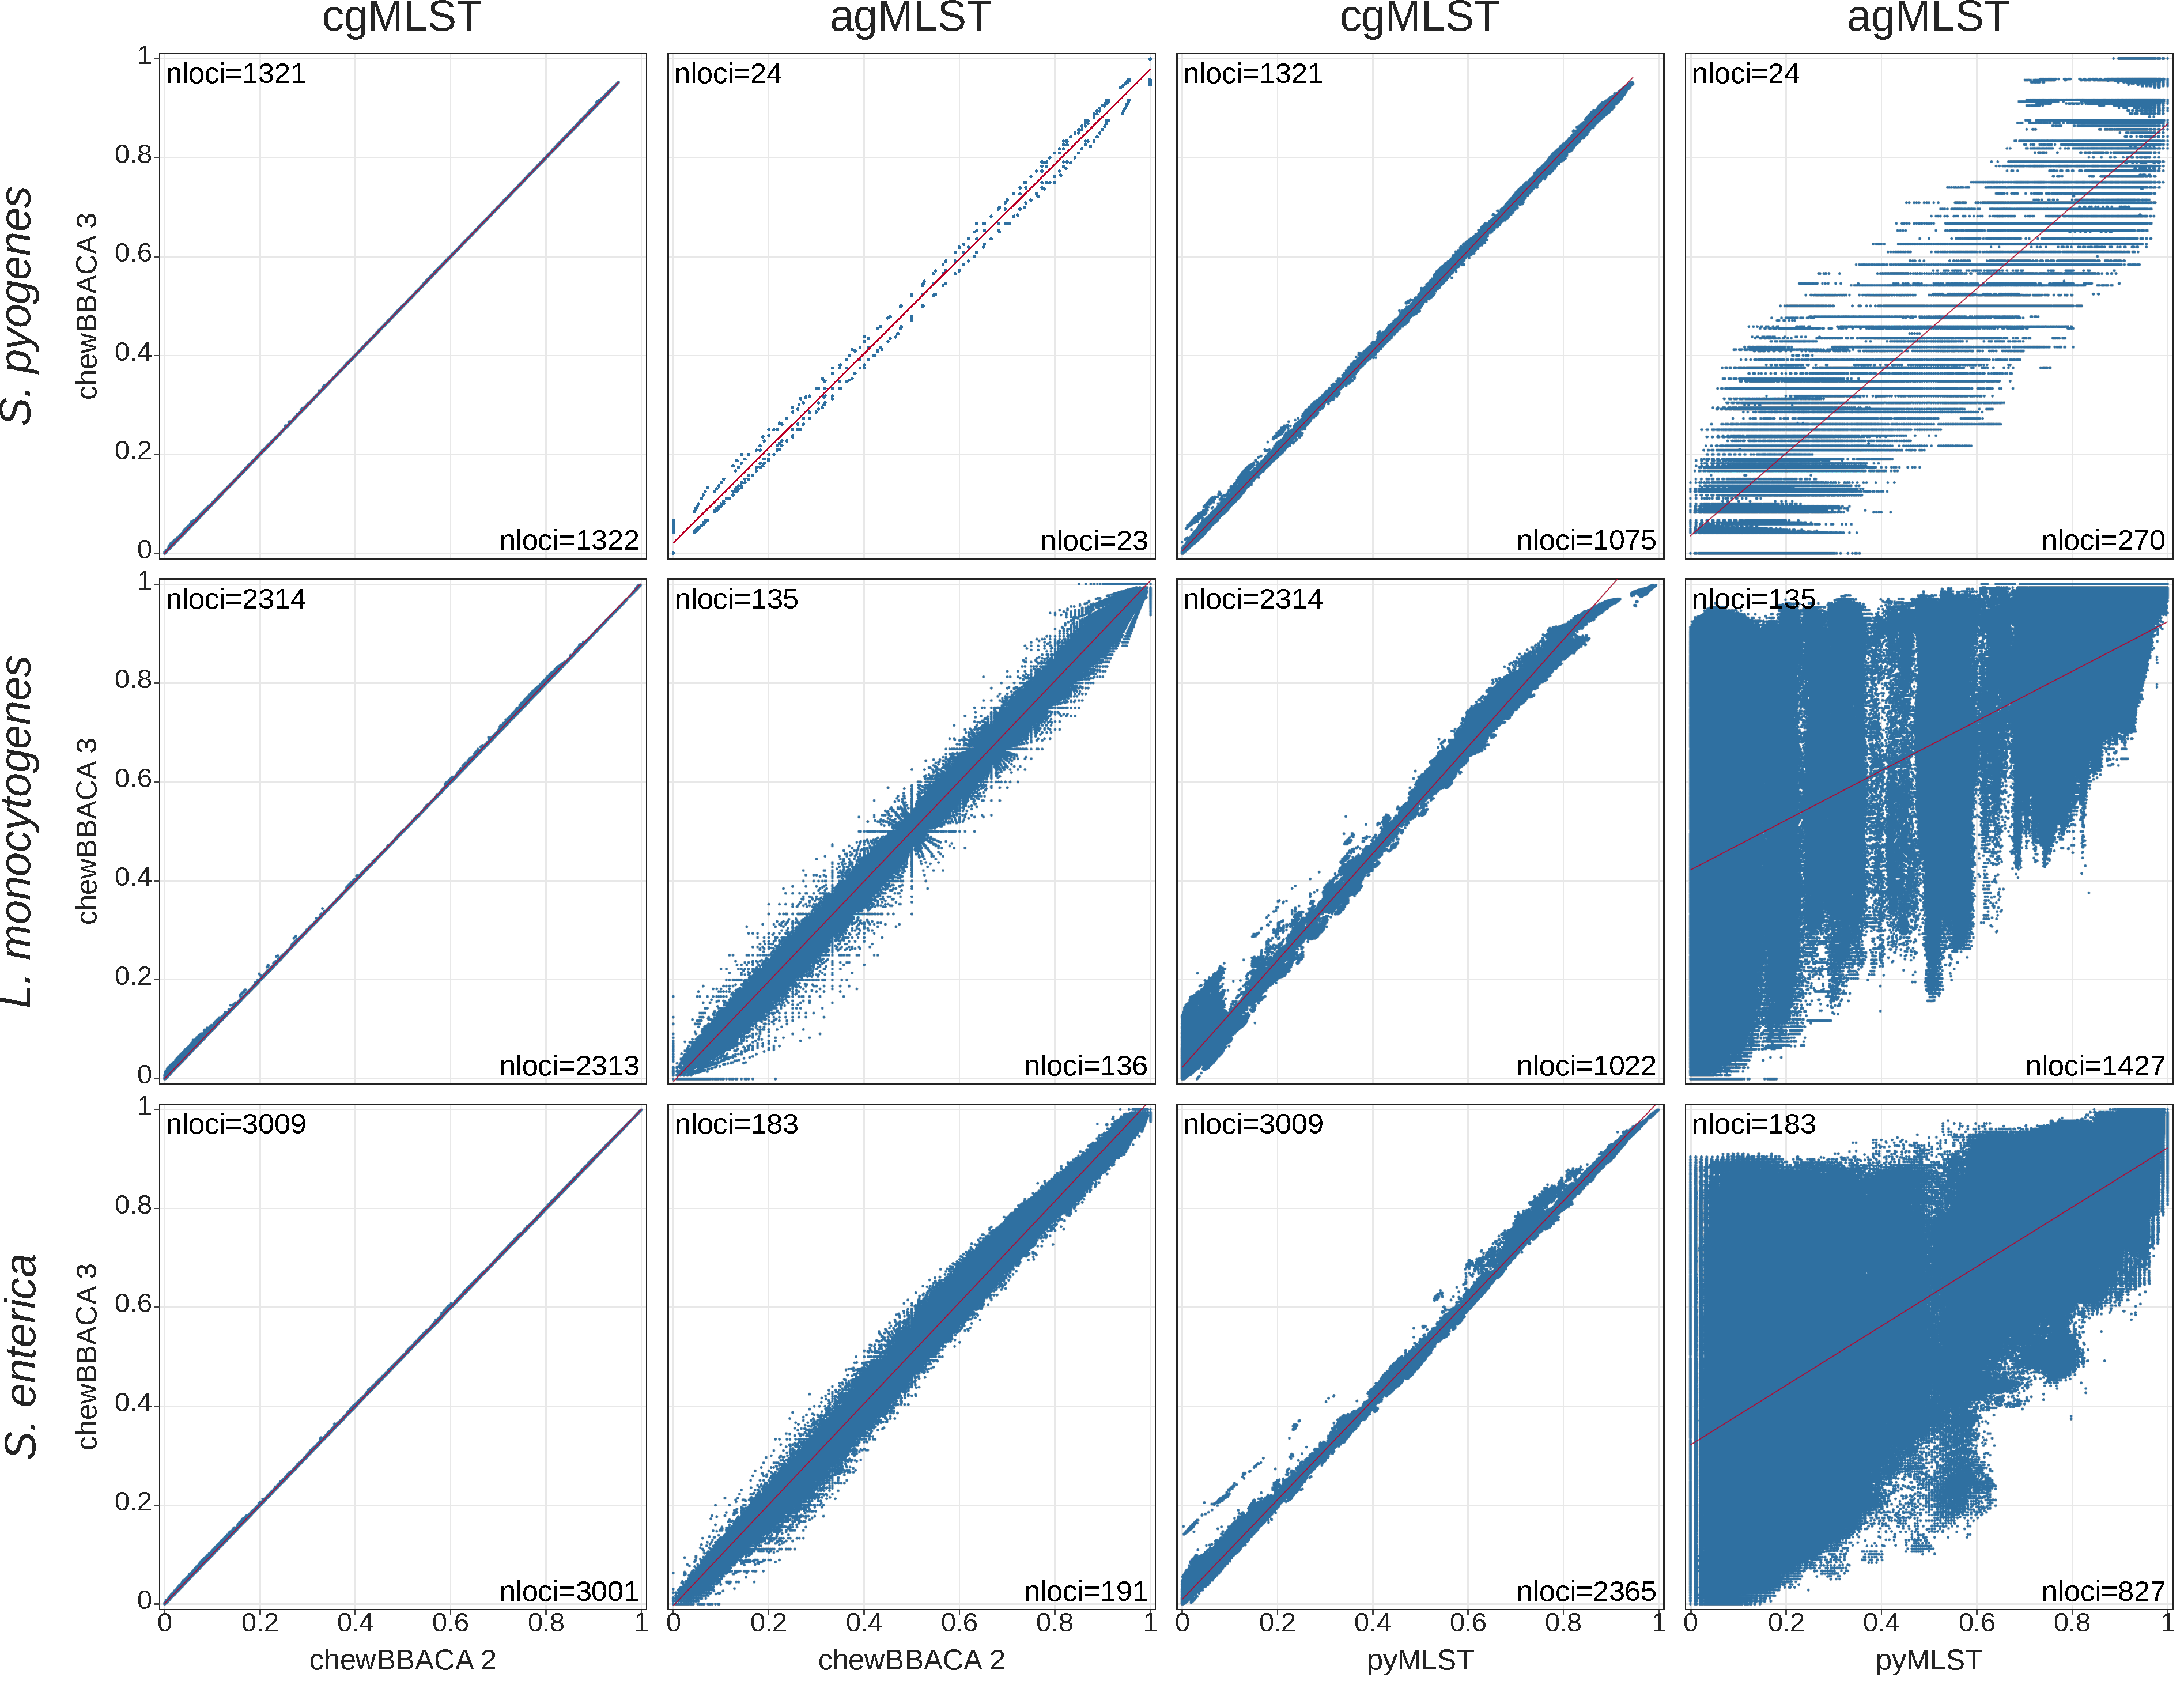
\includegraphics[angle=0,width=\textwidth]{figures/chapter 2/Figure3.pdf}
    \caption{Comparison of the core (cgMLST) and accessory (agMLST) pairwise Jaccard distances. The pairwise Jaccard distances computed based on chewBBACA 3's allele calling results for the complete datasets (n=16,384 genomes) of Streptococcus pyogenes, Listeria monocytogenes, and Salmonella enterica were compared against the the pairwise distances computed from chewBBACA 2's and pyMLST's results. The regression lines are displayed in red. The number of core or accessory loci determined based on chewBBACA 3’s results are shown in the top-left corner of the plot area. The number of core or accessory loci determined based on chewBBACA 2’s or pyMLST’s results are shown in the bottom-right corner of the plot area.}
    \label{fig:chap2_figure3}
\end{figure*}

Compared to chewBBACA 2, chewBBACA 3 identifies special classifications more accurately (Figures S17-S19, Additional File 1 and Table S13, Additional File 2). The identification of paralogous loci was improved by introducing the PAMA classification (Figure S3, Additional File 1) for CDSs that match multiple loci and subdividing the NIPH classification into NIPHEM and NIPH to differentiate between multiple exact matches or a combination of exact and inexact matches (Figure S2, Additional File 1). chewBBACA 3 displays greater sensitivity for detecting multiple matches, leading to more NIPH and NIPHEM classifications than chewBBACA 2, which, in some cases, would detect a single exact match and fail to identify additional inexact matches. The PLOT classification, used by chewBBACA 2 to classify CDSs close to contig ends, was subdivided into PLOT5, PLOT3 and LOTSC to indicate if a CDS is close to the 5'-end, 3'-end, or both (Figure S1, Additional File 1). New output files include the genomic coordinates for the CDSs predicted for all input genomes and relevant classification statistics per genome and locus. The DNA sequences of the CDSs assigned special classifications or not classified can be stored in FASTA files by providing the --output-missing and --output-unclassified options, respectively. These changes improve the granularity of the results to facilitate downstream analyses, such as identifying low-quality inputs, paralogous loci, more divergent alleles, and potential new loci to add to schemas.

Another known issue when using cg/wgMLST approaches is that allelic profiles generated with schemas that do not share the same allele nomenclature are not directly comparable. To enable the comparison of results generated with different schemas, chewBBACA 3 includes the --hash-profiles option that hashes allele sequences to generate hashed allelic profiles. Since the same allele sequence will always result in the same hash value, the allelic profiles can be compared independently of the nomenclatures used by the schemas allowing also greater data privacy. chewBBACA 3 uses the SHA256 algorithm included in Python’s hashlib module by default, but users can select any of the algorithms included in that module or the zlib module.

\subsection{Interactive reports for comprehensive wg/cgMLST schema and allele call results analyses} \label{ssec:results_discussion_ssec4}

The schemas and allele calling results generated by chewBBACA 3 can be a source of valuable data for in-depth analyses that explore the loci diversity captured by a schema and the relatedness of strains of interest. We developed modules that enable a local, scalable and comprehensive analysis of cg/wgMLST schemas and results through interactive reports to support users in performing common downstream analyses to more easily reach an informed decision. To showcase the utility of the reports' functionalities, we analysed 264 S. pyogenes emm1 strains, including strains from the recently emerged M1UK and M1DK lineages \citep{lynskey_emergence_2019, johannesen_increase_2023}, and describe how some of the reports’ components can help identify relevant features to distinguish the lineages.

The SchemaEvaluator (Figure S20, Additional File 1) module evaluates cg/wgMLST schemas created with chewBBACA or from external sources to create an interactive report with detailed information about the schema composition. This module had been introduced in chewBBACA 2, however it ceased functioning due to dependency issues. The module was reimplemented and expanded in chewBBACA 3. The main page of the report includes charts that allow exploring the number of alleles and the allele size variation per locus. The module accepts a file with loci annotations to facilitate the identification of loci of interest. For example, the annotations determined by the UniprotFinder module (Figure S21, Additional File 1) for the S. pyogenes schema can be added to a data table to identify which schema loci have the lineage-defining single-nucleotide polymorphisms (SNPs) of the M1UK (Figure 4A) and M1DK lineages. Another data table displays the results of the allele integrity analysis, which identifies classes of invalid alleles per locus (e.g. incomplete CDSs, presence of ambiguous bases, absence of start and stop codons, in-frame stop codons, and minimum and locus-specific size thresholds). This can be used to identify problematic loci or loci with unusual variability of size.

\begin{figure*}[h!]
    \centering
    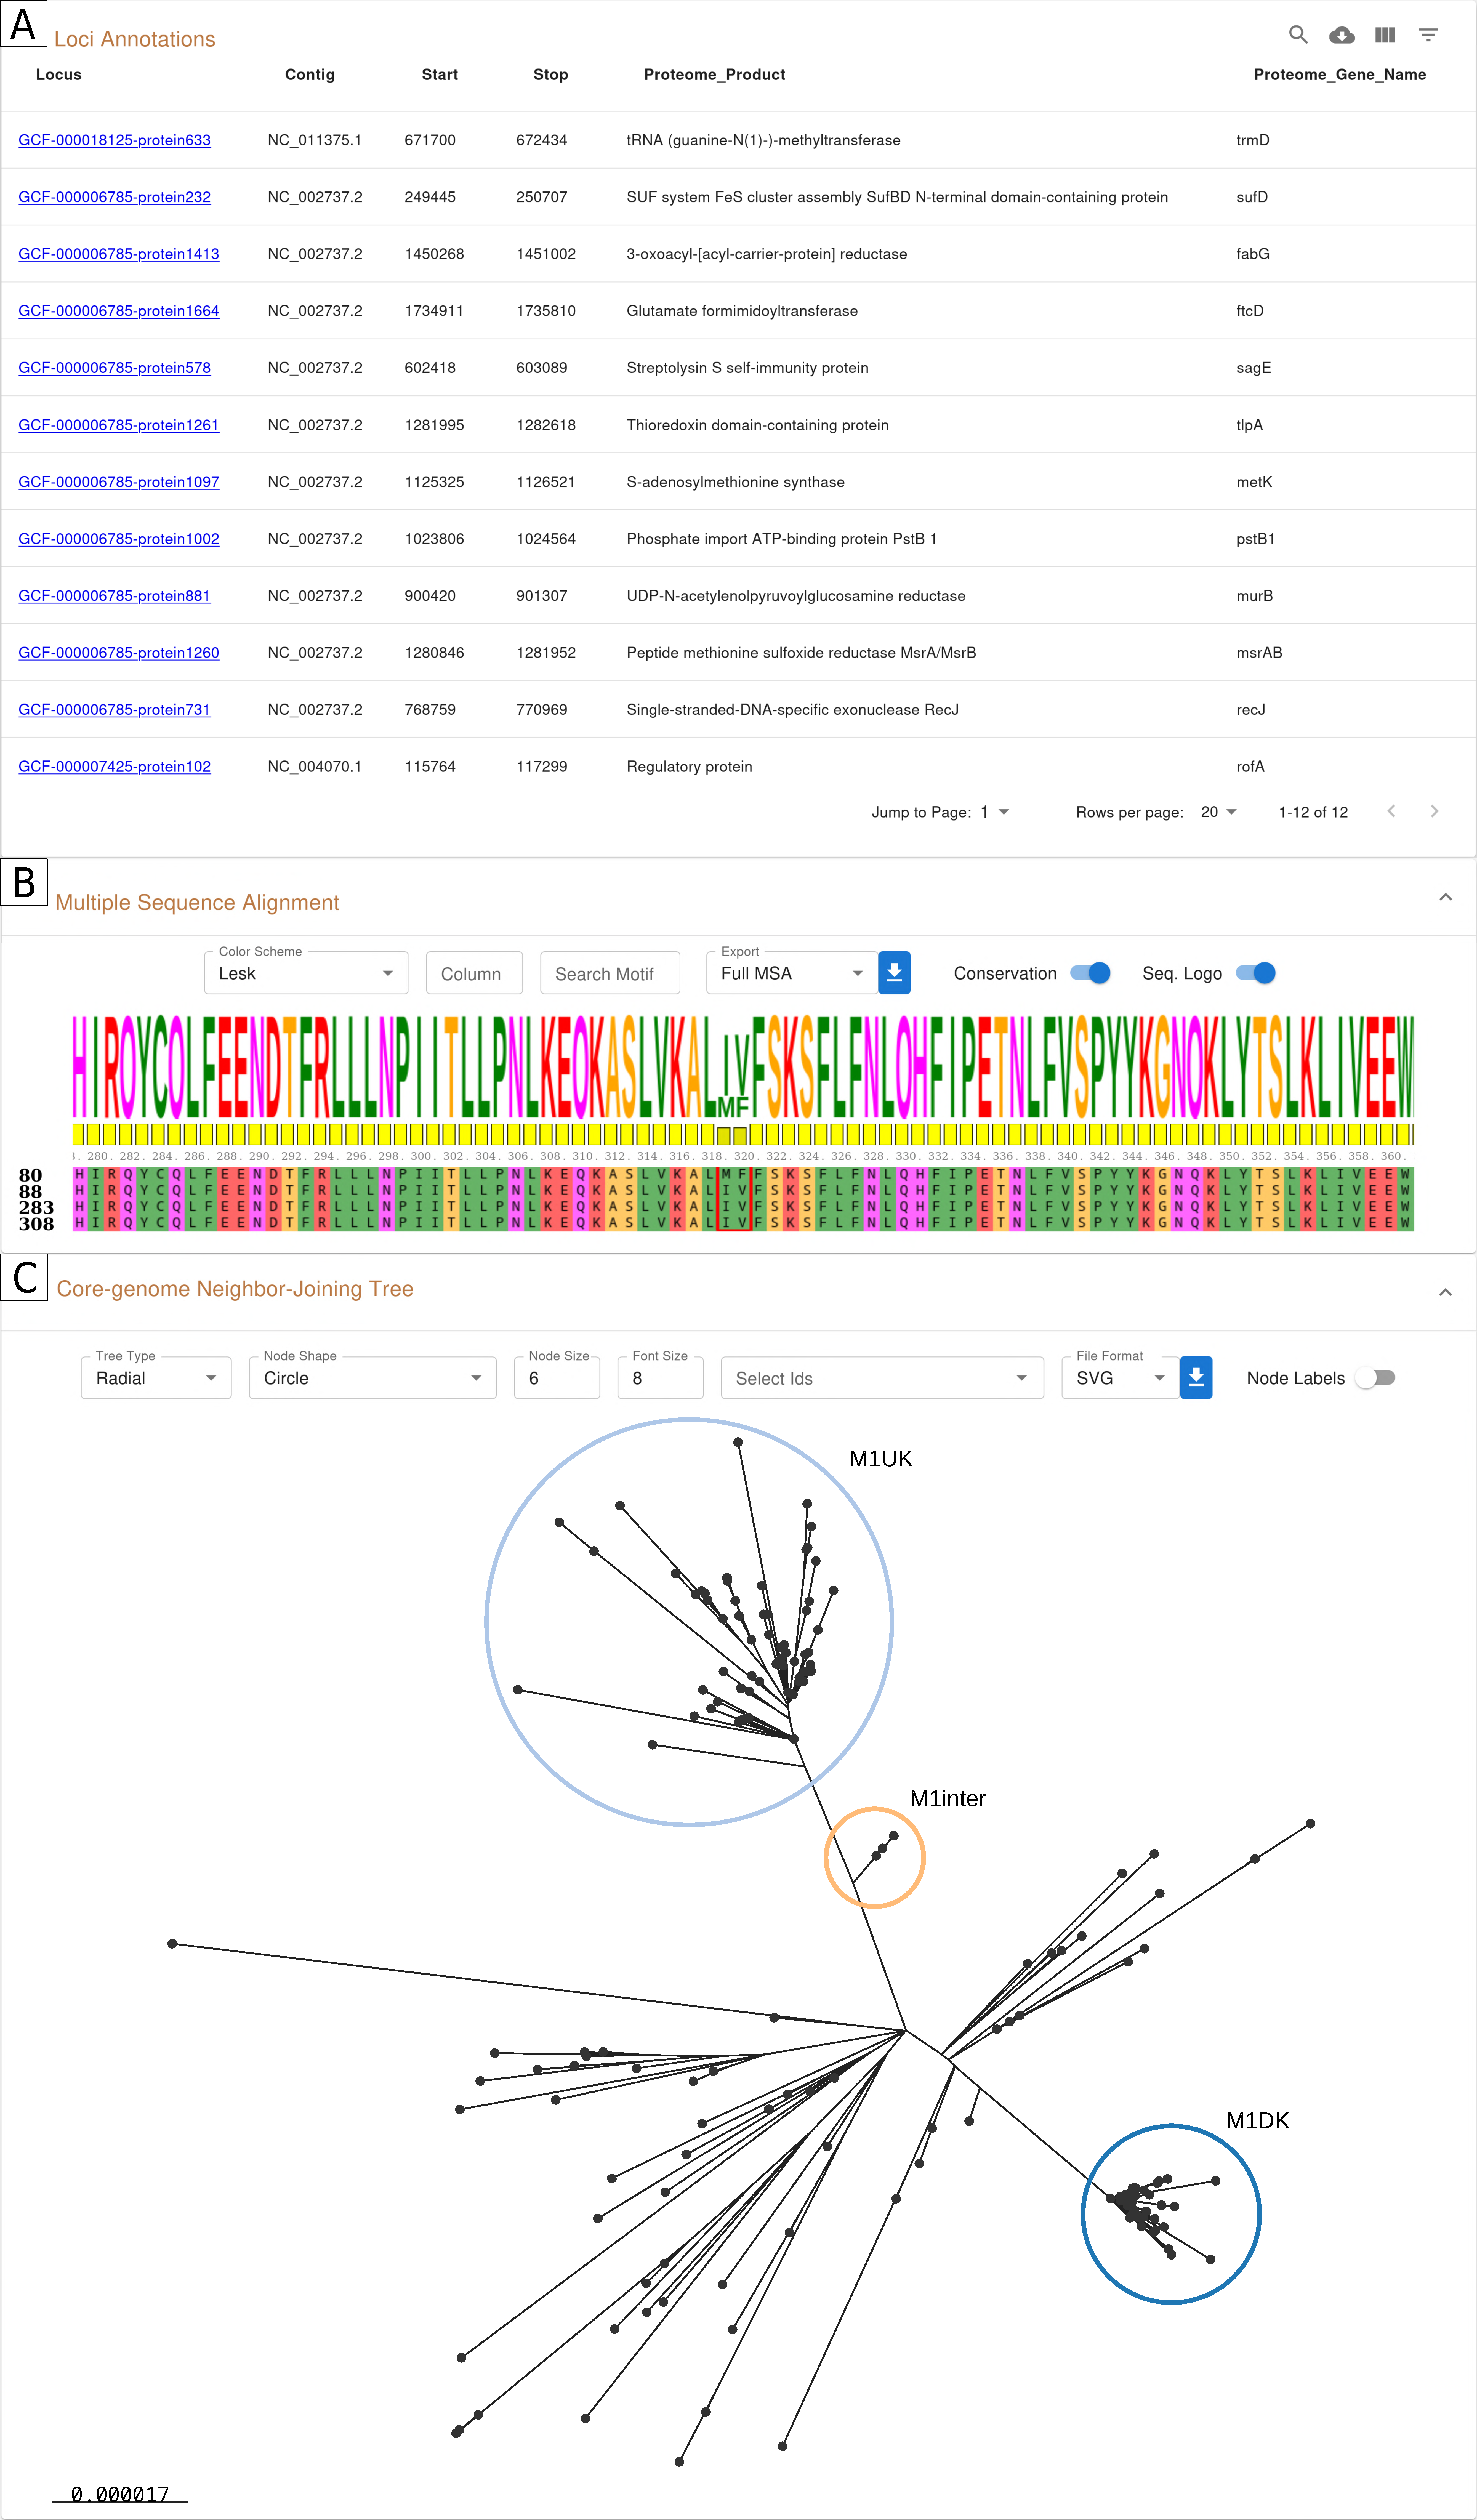
\includegraphics[angle=0,height=0.92\textheight]{figures/chapter 2/Figure4.pdf}
    \label{fig:chap2_figure4}
\end{figure*}
\vspace*{-6mm}
\begin{center}
    \emph{(Caption on next page.)}
\end{center}
\begin{figure*}[h!]
    \caption{Report components generated for the analysis of the \textit{S. pyogenes} schema and lineage strains. (A) Datatable component of the report generated by the \textit{SchemaEvaluator} module including the annotations determined by the \textit{UniprotFinder} module for 12 schema loci containing lineage-defining SNPs for the M1UK lineage. (B) Component of the \textit{SchemaEvaluator} module including a Multiple sequence alignment (MSA) of the rofA translated alleles identified in the MGAS5005 reference strain (allele 80) and the M1UK strains (alleles 88, 283, and 308). Two amino acid differences caused by two SNPs in the rofA alleles of the M1UK strains are highlighted in red. (C) Component of the \textit{AlleleCallEvaluator} module including a Neighbor-Joining tree computed with FastTree from the core loci MSA. The groups of strains belonging to the M1UK (light blue), M1inter (light orange), and M1DK (dark blue) lineages are highlighted. The full reports are available on Zenodo \citep{mamede_supplementary_2025}.}
\end{figure*}

The \textit{-{}-loci-reports} option provides a more detailed analysis of each locus through dedicated locus pages, accessible by clicking on the loci identifiers in the main report data tables. Each locus page contains charts for the allele size distribution, sequence size per allele and number of DNA alleles for each distinct protein. A multiple sequence alignment (MSA) computed with MAFFT \citep{katoh_mafft_2013} for the translated alleles allows identifying shared regions and differences caused by point mutations or indels. For example, the non-synonymous effect of two SNPs in the rofA gene used to define the M1UK lineage can be identified using the MSA by comparing the reference allele with those identified in M1UK strains (Figure 4B). The guide tree created by MAFFT is displayed with Phylocanvas.gl \citep{abudahab_phylocanvasgl_2021} to help identify groups of similar or divergent alleles. To provide a convenient way to identify and copy the DNA and protein sequences of the alleles, users can use the --add-sequences option, which adds code editor components containing the DNA and protein sequences to each locus’ page.

A report with a detailed analysis of the allele calling results is obtained by running the AlleleCallEvaluator module (Figure S22, Additional File 1). The report includes data tables with summary statistics and bar charts with the classification counts per strain and locus to explore the classification results and aid in identifying low-quality genomes (e.g. misassembled or contaminated genomes) and problematic loci (e.g. loci with a high number of special classifications). An interactive analysis of loci presence-absence is performed through a heatmap component that enables identifying the set of core loci or loci specific to certain groups of strains. Similar strains can be identified through another heatmap component that displays the matrix of pairwise core allelic distances and enables searching for similar strains based on a distance threshold. The last component in the report displays a Neighbor-Joining tree computed with FastTree 2 \citep{price_fasttree_2010} from the core loci MSA. This component allows exploring phylogenetic relationships to identify groups of similar strains. For instance, the NJ tree from the analysis of the S. pyogenes strains allows identifying the groups of strains corresponding to each lineage of the M1 group (Figure 4C).

The reports' components include features to sort, select, search, and export data in tabular format, in the case of data tables, or as SVG files, in the case of charts or trees. Some files necessary to create the components, such as the ones containing the matrix of pairwise core allelic distances and the core loci MSA, are provided in the report's folder to allow users to perform custom analyses if desired. The reports are easily shared by simply compressing the report's folder and sharing the resulting archive. The interactive reports created with the SchemaEvaluator and AlleleCallEvaluator modules for the analysis of the S. pyogenes strains are available on Zenodo \citep{mamede_supplementary_2025}.

\section{Conclusions} \label{sec:conclusions}

chewBBACA 3 constitutes an efficient, scalable, and comprehensive solution for wg/cgMLST. The options it provides for schema setup enable users to quickly create schemas from larger collections of genome assemblies or CDS data to capture more of the diversity of a bacterial species, or to adapt or import existing schemas created in other platforms or available in Chewie-NS to promote interoperability. The combination of alignment-based and alignment-free approaches allow for efficient and accurate allele calling, making it suitable for integration into workflows that process sample batches of any size, from sequential processing of single samples to vast genome collections for species-level population analyses. chewBBACA 3 classifies more schema loci and CDSs than the compared methods, potentially providing superior strain discrimination for surveillance and outbreak investigation. The high level of agreement with chewBBACA 2's results, while providing expanded classifications and richer results, facilitates the transition to the latest chewBBACA version. Comparisons with other wg/cgMLST methods should take into account that algorithmic differences between methods, parameter values, and input data quality can greatly affect the resolution and accuracy of the results, which might hinder results comparison and in some cases even lead to fundamentally different conclusions. The reports for schema and allele call evaluation allow a comprehensive and local analysis of locus diversity and strain similarity, enabling scalable and private analyses of the results and reducing the need to combine several tools or develop custom solutions to more fully explore the potential of wg/cgMLST schemas. The integration of chewBBACA 3 into wg/cgMLST workflows will help to further democratize wg/cgMLST by providing broader access to large-scale and detailed analyses to perform focused population studies or facilitate reaching an informed decision in outbreak or transmission investigations.

\section{Methods} \label{sec:methods}

\subsection{Download and selection of complete and draft genome assemblies} \label{ssec:methods_ssec1}

Complete and draft genome assemblies annotated as \textit{Streptococcus pyogenes}, \textit{Listeria monocytogenes} and \textit{Salmonella enterica} were downloaded with the NCBI Datasets command-line tools v16.12.0 \citep{oleary_exploring_2024} on September 9, 2023. The complete genomes were downloaded from the NCBI RefSeq database \citep{sayers_database_2022} using the –assembly-source “RefSeq” and –assembly-level complete options. The draft genome assemblies were downloaded from the NCBI GenBank database \citep{sayers_database_2022} using the –assembly-source “GenBank” option. The –exclude-atypical and –mag exclude options were used in both cases. The number of draft genome assemblies for \textit{S. pyogenes} available from GenBank was insufficient to create the complete dataset (n=16384) for the benchmark. Due to that, draft genome assemblies annotated as \textit{Streptococcus pyogenes} were also downloaded from a collection of 661K genomes available on the European Nucleotide Archive (ENA) \citep{blackwell_exploring_2021}. MLST v2.23.0 \citep{jolley_bigsdb_2010, seemann_mlst_nodate} was used to determine the Sequence Type (ST) for all assemblies. Assemblies without a known ST or assigned an ST from a different species, indicating possible misannotation, were excluded. A custom Python script was also used to filter out assemblies based on a maximum number of contigs of 100, a maximum number of ambiguous bases of 1000, and a minimum and maximum genome size. The minimum and maximum genome size values were defined based on the \textit{min\_ungapped\_length} and \textit{max\_ungapped\_length} values in the “species\_genome\_size.txt” file available on NCBI’s FTP on September 9, 2023 (\url{https://ftp.ncbi.nlm.nih.gov/genomes/ASSEMBLY_REPORTS/}) \citep{sayers_database_2022}.

\subsection{Dataset creation} \label{ssec:methods_ssec2}

The selected draft genome assemblies were subsampled to create datasets to evaluate the performance of chewBBACA 3, chewBBACA 2 and pyMLST. The pairwise average nucleotide identity (ANI) distances for each species’ selected draft genomes were computed with Skani v0.2.1 \citep{shaw_fast_2023}. To factor in the aligned genome fraction, weighted ANI values were computed by multiplying the ANI values by the mean of the query and reference aligned fractions. The weighted ANI values were ordered to select a set of 16,384 genomes that maximized the average pairwise distance. Smaller datasets were created by randomly sampling this dataset, starting by selecting 1 genome and doubling the dataset size until reaching a dataset size of 8,192. Five replicates were created for each dataset size. The complete datasets with 16,384 genomes were compressed with AGC v3.0 \citep{deorowicz_agc_2023} to allow efficient storage and fast genome retrieval based on lists of genome identifiers.

\subsection{Creation of wg/cgMLST schemas} \label{ssec:methods_ssec3}

A total of 260, 309 and 1,326 complete genomes for \textit{Streptococcus pyogenes}, \textit{Listeria monocytogenes} and \textit{Salmonella enterica}, respectively, were selected for schema creation. wgMLST schema seeds were created with the \textit{CreateSchema} module available in chewBBACA v3.3.6 and compared against the schema seeds created by the previous \textit{CreateSchema} implementation, available in chewBBACA v2.6.0 \citep{silva_chewbbaca_2018}. The schema creation processes used a minimum sequence length value of 0 (\textit{--l 0}) and the Prodigal \citep{hyatt_prodigal_2010} training files bundled with chewBBACA. The schema seeds created by both versions were compared based on a BSR $\geq0.6$ and a proportion of shared minimizers $\geq0.9$ to determine sets of loci shared by the schema seeds created with both versions. Schema seeds created with chewBBACA v3.3.0 were populated with the alleles identified in the complete genomes through allele calling. The results of the allele calling were used to determine the set of core loci with the ExtractCgMLST module based on a loci presence threshold of 1 (\textit{--t 1}) and create the cgMLST schemas used to evaluate the allele calling performance. The cgMLST schemas were adapted with the \textit{PrepExternalSchema} module implemented in chewBBACA v2.8.5 to create the cgMLST schemas for that version. To create equivalent databases for pyMLST \citep{biguenet_introduction_2023}, multi-FASTA files with the first representative allele for each locus in the cgMLST schemas were passed to the wgMLST create command. The wgMLST add command was used to add each complete genome to the pyMLST databases.

\subsection{External schema adaptation} \label{ssec:methods_ssec4}

The cgMLST schemas for \textit{S. pyogenes}, \textit{L. monocytogenes} and \textit{S. enterica} available on the cgMLST.org server \citep{noauthor_cgmlstorg_nodate} were downloaded on July 4, 2024. These schemas were adapted with the \textit{PrepExternalSchema} module available in chewBBACA v3.3.6 and compared against the schemas adapted with the previous \textit{PrepExternalSchema} implementation, available in chewBBACA v2.0.17.2. The representativeness of the set of representative alleles selected by the \textit{PrepExternalSchema} module was measured by aligning the representative alleles selected for each locus against all valid locus alleles based on a BSR $\geq0.6$.

\subsection{Evaluation of the allele calling results} \label{ssec:methods_ssec5}

The cgMLST schemas and datasets containing between 1 and 16,384 draft genome assemblies were used to evaluate the allele calling performance of chewBBACA v3.3.3, chewBBACA v2.8.5 and pyMLST v2.1.5. The number of distinct CDSs per dataset was computed based on the CDSs predicted by Pyrodigal v3.0.0. Runtime, peak memory usage, and the comprehensiveness of the allele calling were evaluated for all datasets. The allelic profiles for the strains classified by pyMLST were extracted from the databases with the wgMLST mlst command and converted to the format used by chewBBACA with a custom script. The allelic profiles were masked to remove the \textit{INF-} prefix from inferred alleles and to substitute all special classifications or missing values by 0. The core loci were defined with the \textit{ExtractCgMLST} module based on the complete datasets' results and a loci presence threshold of 0.95. Loci below this threshold were considered to be part of the accessory genome. The pairwise Jaccard and allelic distances were computed with a custom script based on the masked allelic profiles. The proportion of classified CDSs and identified loci are based on the total number of CDSs predicted by Pyrodigal and on the total number of loci in each schema, respectively.

\subsection{Download and analysis of \textit{S. pyogenes} \textit{emm1} strains} \label{ssec:methods_ssec6}

The genome assemblies and metadata for the \textit{S. pyogenes} strains belonging to each lineage were recovered from previous studies \citep{lynskey_emergence_2019, johannesen_increase_2023, friaes_annotated_2022}. The schema loci containing the lineage-defining SNPs were identified using BLASTp to align the translated CDSs from the MGAS5005 reference genome \citep{sumby_evolutionary_2005}, with RefSeq accession number \textit{GCF\_000011765.3}, against the translated schema alleles.

\subsection{Runtime and peak memory usage measurement} \label{ssec:methods_ssec7}

Runtime and peak memory usage were measured with the GNU time command on a desktop computer with an Intel® Core™ i7-4790 CPU, 32GB 1600 MT/s RAM, and a 1TB Samsung SSD 870 QVO. Any analysis that evaluated runtime and peak memory usage used 6 CPU cores to run chewBBACA 3 and chewBBACA 2 and 1 CPU core for pyMLST because the latter cannot use multiple cores.

\section{Availability and requirements} \label{sec:availability_and_requirements}

\noindent Project name: chewBBACA 3.\\
Project home page: \url{https://github.com/B-UMMI/chewBBACA}\\
Project documentation: \url{https://chewbbaca.readthedocs.io/en/latest/index.html}\\
Operating system(s): Linux and macOS.\\
Programming language: Python >= 3.8\\
Other requirements: BLAST+ >= 2.9.0, pyrodigal>=3.0.0, numpy~=1.24.3, scipy~=1.10.1, biopython>=1.79, plotly>=5.8.0, SPARQLWrapper>=2.0.0, requests>=2.27.1, pandas>=1.5.1\\
License: GPL-3.0\\
Any restrictions to use by non-academics: None.

\section{List of abbreviations} \label{sec:list_of_abbreviations}

\noindent ANI: average nucleotide identity\\
BLASTp: Protein BLAST\\
BSR: BLAST Score Ratio\\
CDS: coding DNA sequence\\
ECDC: European Centre for Disease Prevention and Control\\
EFSA: European Food Safety Authority\\
ENA: European Nucleotide Archive\\
GbG: gene-by-gene\\
MSA: multiple sequence alignment\\
NCBI: National Center for Biotechnology Information\\
NJ: Neighbor-Joining\\
SNP: single nucleotide polymorphism\\
SNV: single nucleotide variant\\
ST: Sequence Type\\
wg/cgMLST: whole genome and core genome multilocus sequence typing\\
WGS: whole genome sequencing

\section{Declarations} \label{sec:declarations}

\subsection{Ethics approval and consent to participate} \label{ssec:declarations_ssec1}

\noindent Not applicable.

\subsection{Consent for publication} \label{ssec:declarations_ssec2}

\noindent Not applicable.

\subsection{Availability of data and materials} \label{ssec:declarations_ssec3}

The datasets, schemas and databases created and used with chewBBACA 3, chewBBACA 2, and pyMLST, and all results generated for each section are available on Zenodo (\url{https://doi.org/10.5281/zenodo.14637859}) \citep{mamede_supplementary_2025}. The supplementary figures and tables are included in the additional files.

\subsection{Competing interests} \label{ssec:declarations_ssec4}

MR received honoraria for serving on the speakers bureau of Pfizer and Merck Sharp and Dohme and for serving in expert panels of GlaxoSmithKline and Merck Sharp and Dohme. All other authors declare they have no competing interests.

\subsection{Funding} \label{ssec:declarations_ssec5}

This work was partly supported by the ISIDORe project (funding from the European Union’s Horizon Europe Research \& Innovation Programme, Grant Agreement no. 101046133). RM was supported by the Fundação para a Ciência e Tecnologia (FCT) (grant 2020.08493.BD).

\subsection{Author’s contributions} \label{ssec:declarations_ssec6}

All authors contributed to the design of the tool. RM implemented, tested, and benchmarked the tool. PVC contributed to the implementation of the tool. RM and MR wrote the manuscript. All authors read, revised and approved the final manuscript.


%%%%

%INNUca v2.6 pipeline\footnote{\url{https://github.com/B-UMMI/INNUca/}}
%$\sim$3,500
%pATLAS tool\footnote{\url{http://www.patlas.site/}}
%\ref{tab:ch2_table_1})
%\ref{fig:chap2_figure1}
%$leq$ 7

\newpage

\section{Supplemental Material}

\begin{figure*}[h!]
    \centering
    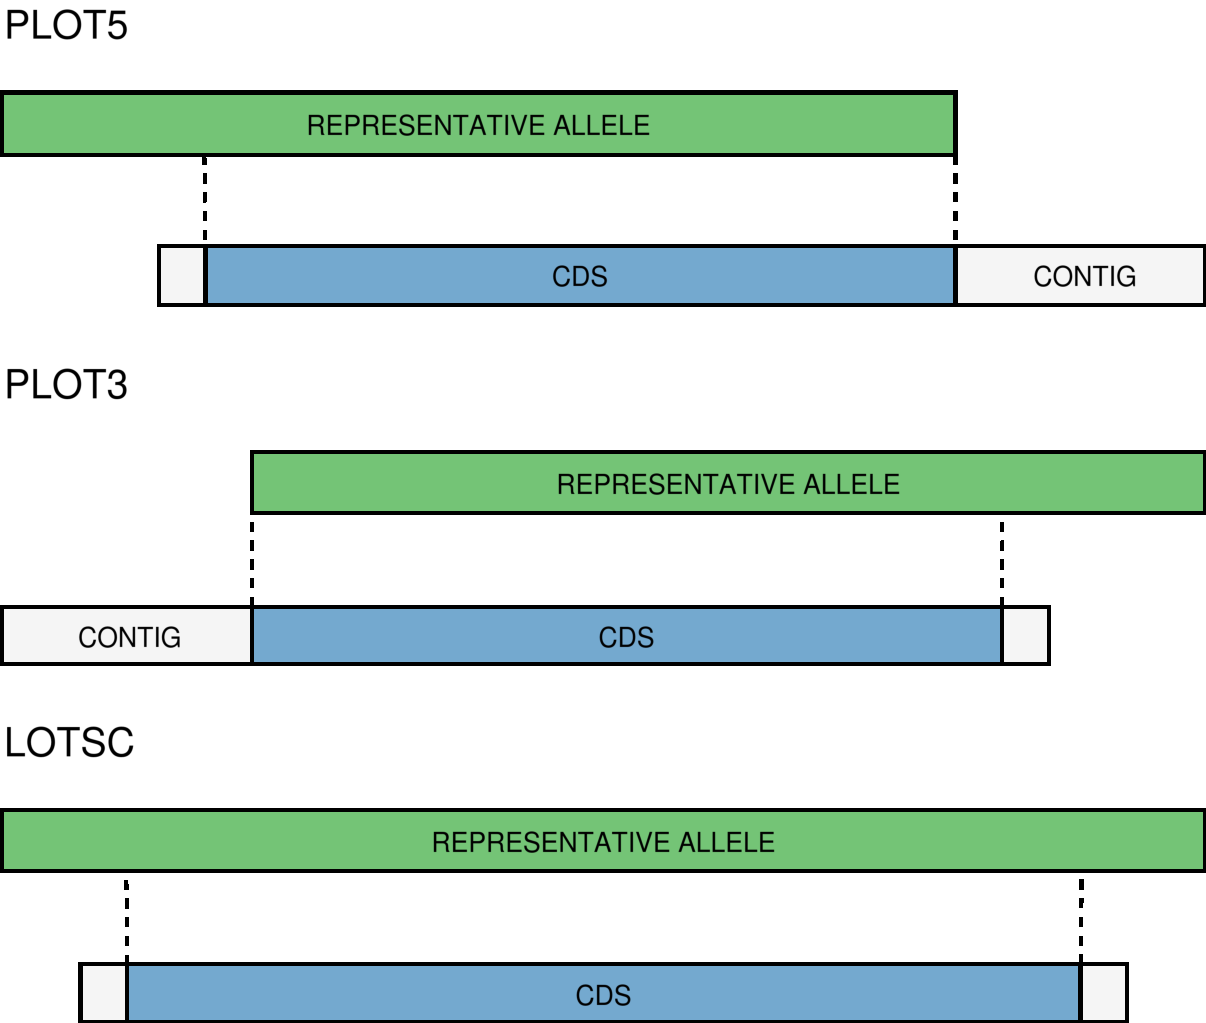
\includegraphics[angle=0,width=\textwidth]{figures/chapter 2/FigureS1.pdf}
    \caption{PLOT5, PLOT3 and LOTSC classifications. The PLOT3, PLOT5 and LOTSC classifications are related to the position of CDSs in the genomic contigs. PLOT5 and PLOT3 (Possible Locus On the Tip) - a CDS is classified as PLOT5 or PLOT3 if it is close to the contig 5’- or 3’-end and if the unaligned portion of the matched representative allele exceeds the contig end. LOTSC - a CDS is classified as LOTSC if the matched representative allele is bigger than the contig containing the CDS.}
    \label{fig:chap2_figureS1}
\end{figure*}

\newpage
\begin{figure*}[h!]
    \centering
    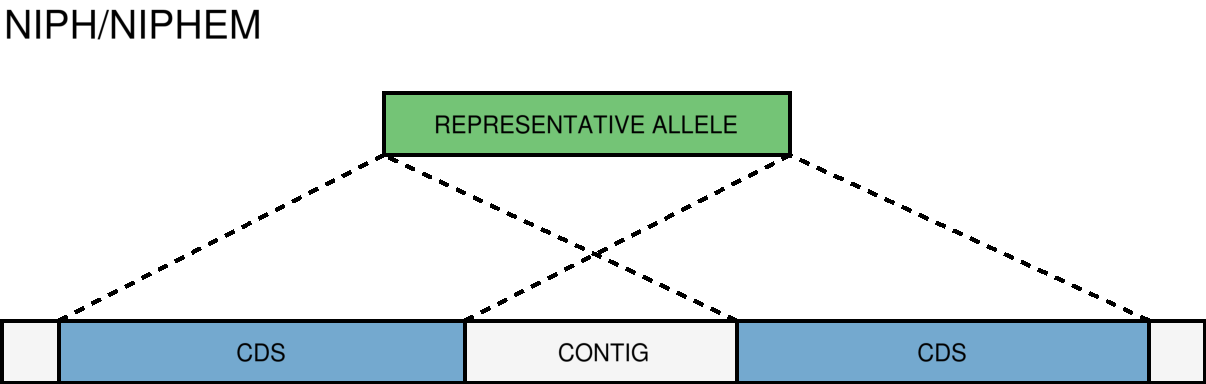
\includegraphics[angle=0,width=\textwidth]{figures/chapter 2/FigureS2.pdf}
    \caption{NIPH and NIPHEM classifications. The NIPH and NIPHEM classifications are assigned when multiple CDSs from the same genome match the same schema locus. NIPH (Non-Informative Paralogous Hit) - assigned when multiple CDSs from the same genome match a single locus. NIPHEM (Non-Informative Paralogous Hit Exact Match) - assigned when multiple CDSs from the same genome are exact matches to alleles of a single locus.}
    \label{fig:chap2_figureS2}
\end{figure*}

\newpage
\begin{figure*}[h!]
    \centering
    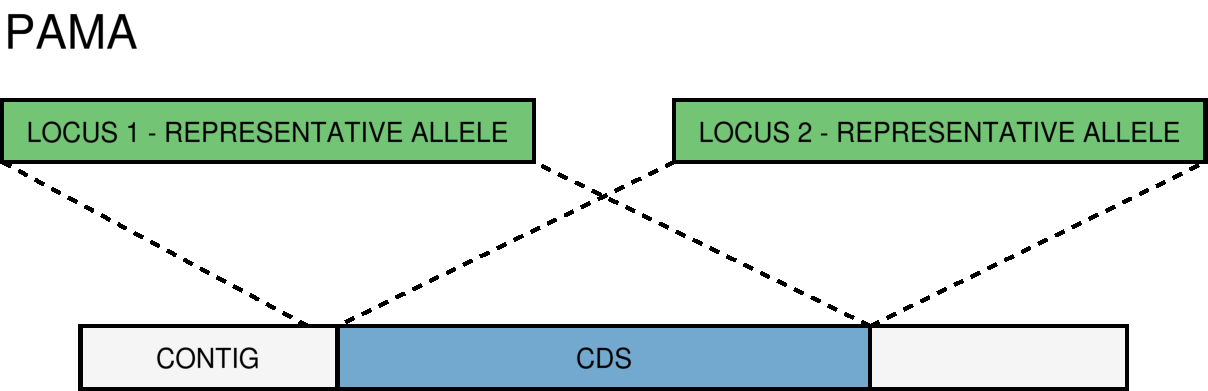
\includegraphics[angle=0,width=\textwidth]{figures/chapter 2/FigureS3.pdf}
    \caption{PAMA classification. The PAMA (PAralogous MAtch) classification is assigned when a single CDS from a genome matches multiple schema loci.}
    \label{fig:chap2_figureS3}
\end{figure*}

\newpage
\begin{figure*}[h!]
    \centering
    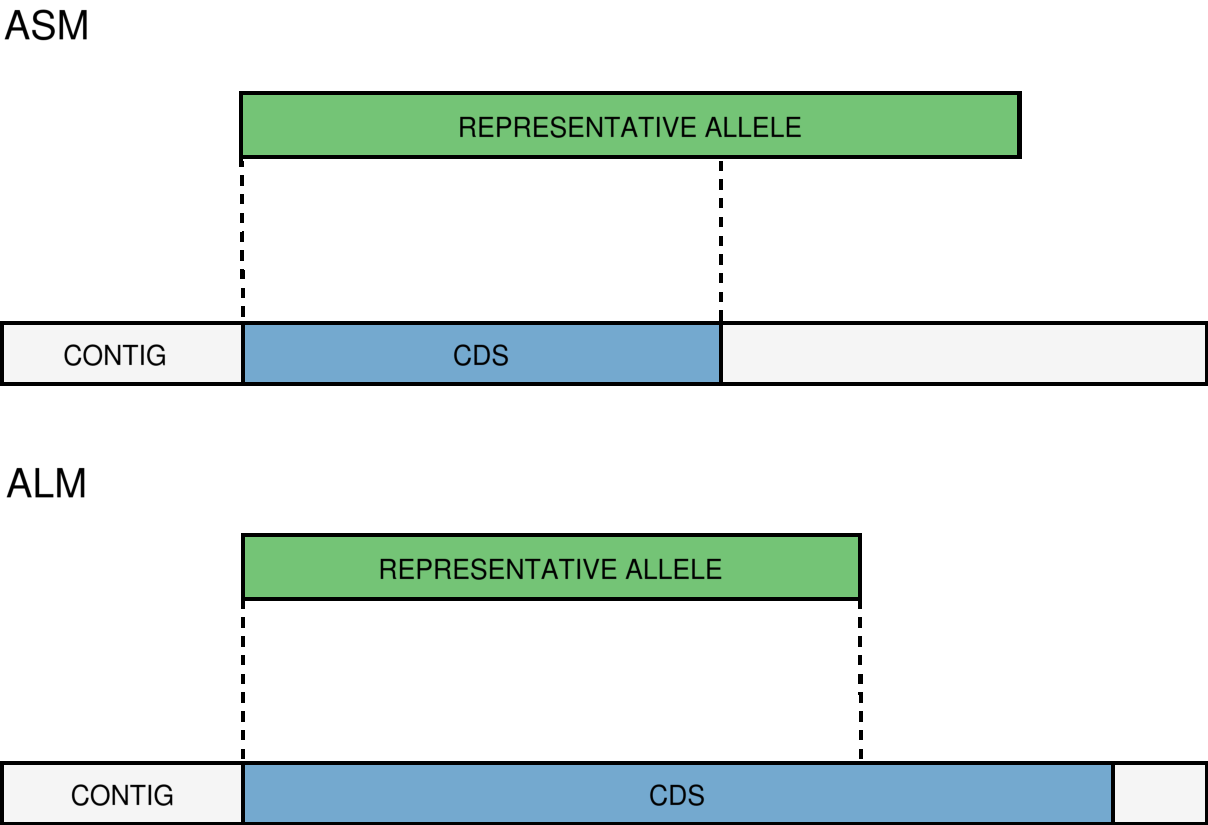
\includegraphics[angle=0,width=\textwidth]{figures/chapter 2/FigureS4.pdf}
    \caption{ASM and ALM classifications. The ASM (Allele Smaller than Mode) and ALM (Allele Larger than Mode) classifications are assigned when the size of a CDS that matches a schema locus is below or above the locus size variation interval, respectively. The default behaviour is to assign these classifications to alleles that are 20\% shorter or longer than the locus allele size mode.}
    \label{fig:chap2_figureS4}
\end{figure*}

\newpage
\begin{figure*}[h!]
    \centering
    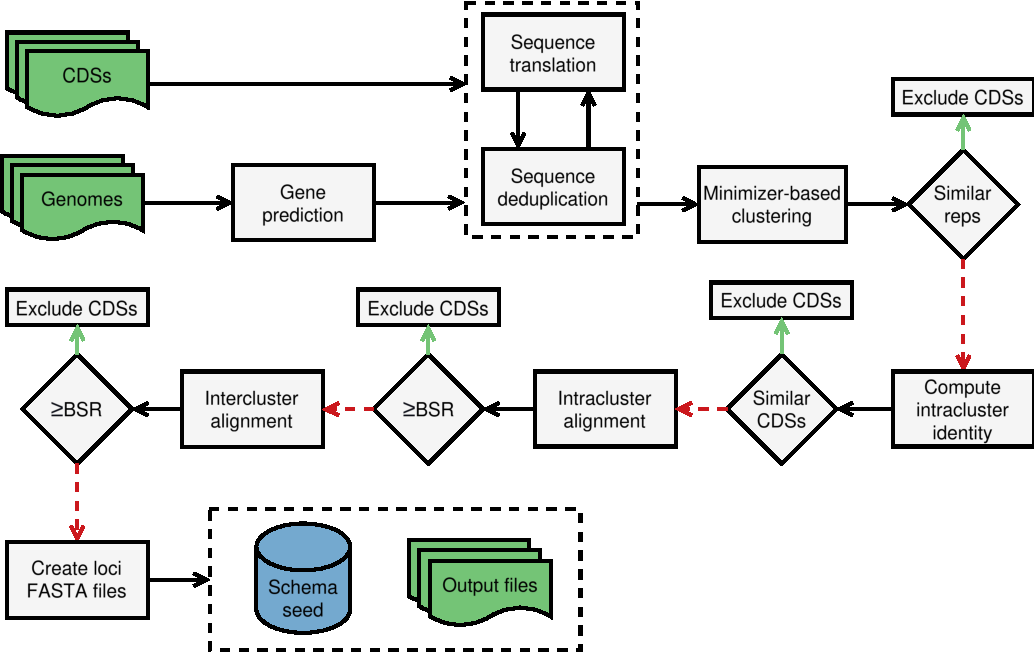
\includegraphics[angle=0,width=\textwidth]{figures/chapter 2/FigureS5.pdf}
    \caption{Diagram of the CreateSchema module. The CreateSchema module creates a schema seed based on a set of FASTA files with genome assemblies or CDSs. If genome assemblies are given, the process starts by predicting CDSs for each genome using Pyrodigal. The CDSs identified in the input files are deduplicated and translated, followed by a second deduplication step to determine the set of distinct translated CDSs. The distinct translated CDSs are clustered based on the proportion of minimizers shared with representative CDSs. The largest or one of the largest CDSs is selected as the first representative CDS. New representative CDSs are selected when CDSs share a low proportion (<0.2) of minimizers with any of the chosen representative CDSs. Non-representative CDSs that share a proportion of minimizers $\geq0.9$ with the cluster representative are considered to correspond to the same locus and are excluded from the analysis. The proportion of shared minimizers between non-representative CDSs is determined to exclude CDSs sharing a proportion of minimizers $\geq0.9$ with larger CDSs. Intracluster and intercluster alignment with BLASTp enable identifying and excluding CDSs similar to representative or larger non-representative CDSs based on a BLAST Score Ratio (BSR) $\geq0.6$. Each remaining CDS is considered to be an allele of a distinct locus. The process ends by creating a schema seed, which includes one FASTA file containing a single representative allele per distinct locus identified in the analysis. Green document icons represent input FASTA files and output files. Grey rectangle icons represent analysis steps. Diamond icons represent conditional statements, with green arrows used when the condition is met and red dashed arrows otherwise. The blue cylinder icon represents the schema seed created by the CreateSchema module.}
    \label{fig:chap2_figureS5}
\end{figure*}

\newpage
\begin{figure*}[h!]
    \centering
    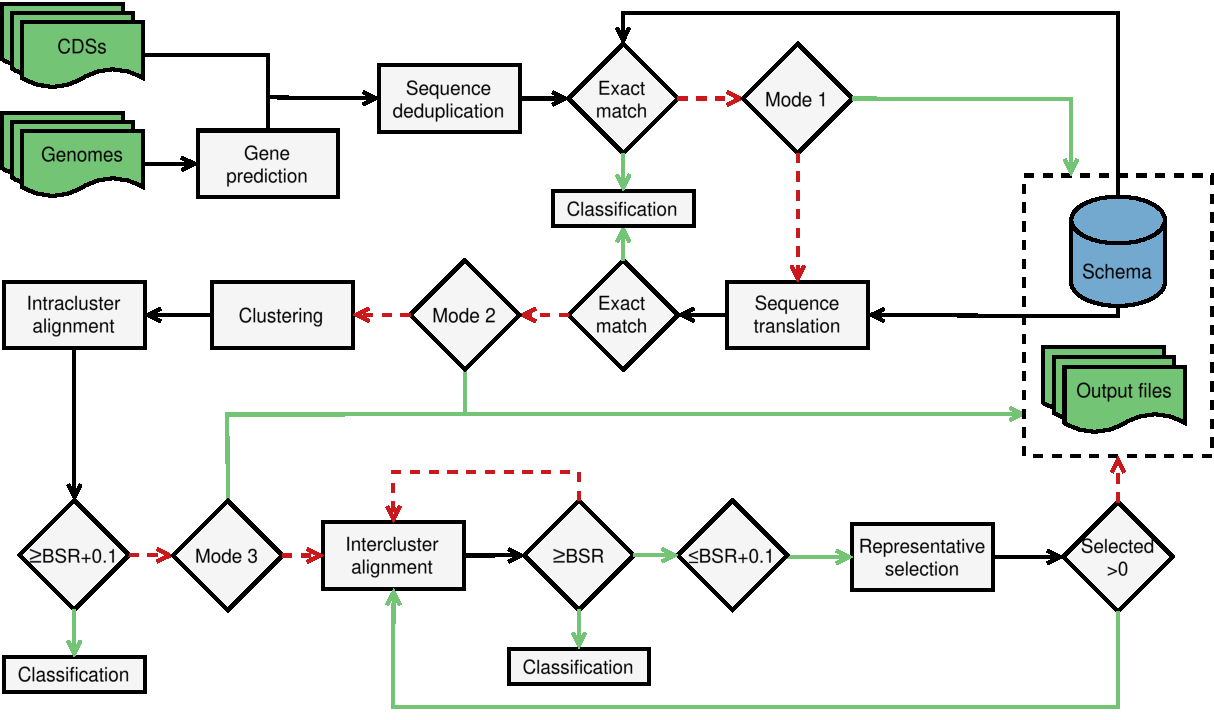
\includegraphics[angle=0,width=\textwidth]{figures/chapter 2/FigureS6.pdf}
    \caption{Diagram of the AlleleCall module. The AlleleCall module determines the allelic profiles for strains of interest. The process accepts FASTA files with genome assemblies or CDSs. If genome assemblies are given, the process starts by predicting CDSs for each genome using Pyrodigal. The CDSs identified in the input files are deduplicated and compared against the schema alleles to find and classify exact matches at the DNA level. If the process runs in mode 1, the results are evaluated to write the output files and exit. Otherwise, the CDSs that do not match any schema alleles at the DNA level are translated and matched against the translated schema alleles to find exact matches at the protein level. If the process runs in mode 2, the results are evaluated to write the output files, add new alleles to the schema and exit. Otherwise, the CDSs not classified through exact matching are compared against the schema representative alleles through minimizer-based clustering to identify CDSs that share a proportion of minimizers $\geq0.2$ with the representative alleles. Each cluster's representative allele is aligned against the clustered CDSs with BLASTp to classify CDSs based on the defined BLAST Score Ratio (BSR) value plus 0.1. At this point, if the process runs in mode 3, the results are evaluated to write the output files, add new alleles to the schema and exit. Otherwise, the representative alleles are aligned against the remaining unclassified CDSs to classify them based on the defined BSR value and identify new representative alleles whose BSR is not above the defined BSR value plus 0.1. If the process finds new representative alleles, it aligns them against the unclassified CDSs to find new matches. This process repeats until no new representative alleles are identified. When no new representative alleles are found, the process evaluates the results to create the output files, add new alleles to the schema, and exit. Green document icons represent input FASTA files and output files. Grey rectangle icons represent analysis steps. Diamond icons represent conditional statements, with green arrows used when the condition is met and red dashed arrows otherwise. The blue cylinder icon represents a schema.}
    \label{fig:chap2_figureS6}
\end{figure*}

\newpage
\begin{figure*}[h!]
    \centering
    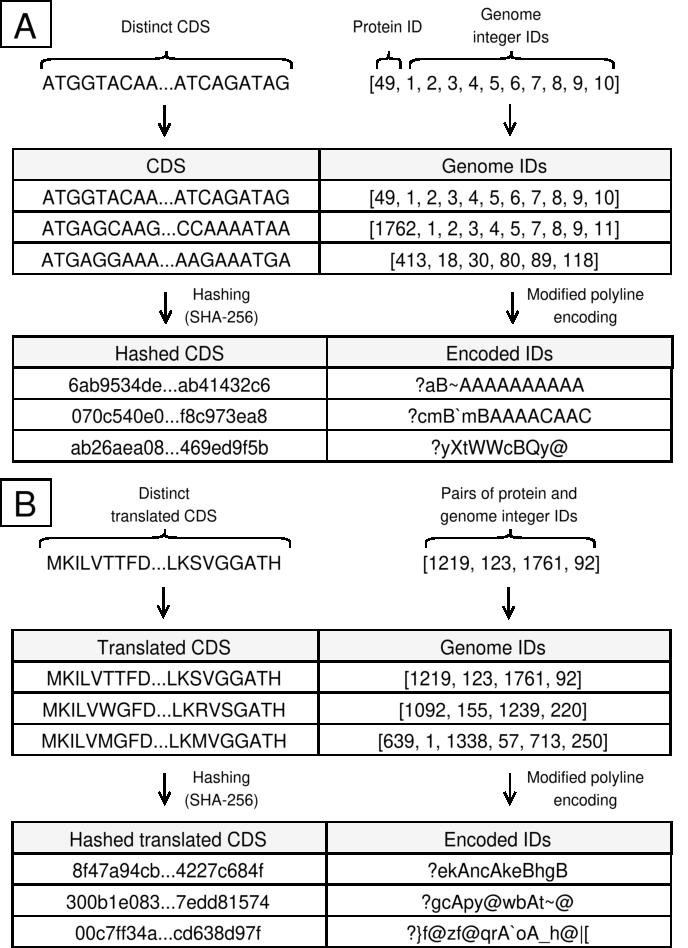
\includegraphics[angle=0,width=0.9\textwidth]{figures/chapter 2/FigureS7.pdf}
    \caption{Sequence hashing and modified polyline encoding. (A) Each distinct CDS identified in the input genomes is hashed with the SHA-256 algorithm implemented in Python's hashlib library. The hash digest is obtained through the hexdigest method and mapped to the list of integer identifiers for the genomes containing the CDS encoded with modified polyline encoding. (B) After sequence translation and deduplication, each distinct translated CDS is hashed with the SHA-256 algorithm and the hash digest is mapped against lists with pairs of protein and genome identifiers used to identify each distinct CDS coding for the protein encoded with modified polyline encoding. The modified polyline encoding is applied to reduce the memory used to retain the data in-memory during the process, drastically reducing peak memory usage when processing large datasets. The Python dictionaries created to map the hashes to the lists of identifiers allow quick identification and classification of exact and inexact matches.}
    \label{fig:chap2_figureS7}
\end{figure*}

\newpage
\begin{figure*}[h!]
    \centering
    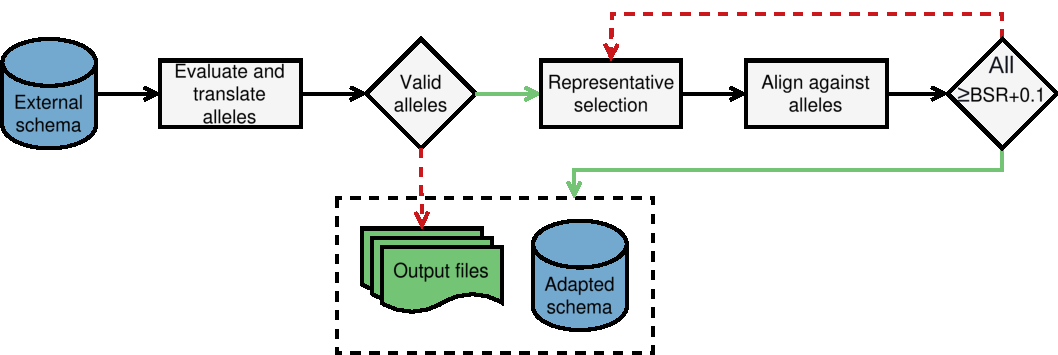
\includegraphics[angle=0,width=\textwidth]{figures/chapter 2/FigureS8.pdf}
    \caption{Diagram of the PrepExternalSchema module. The PrepExternalSchema module adapts schemas created with other wg/cgMLST tools or available on external platforms for usage with chewBBACA 3. The process starts by validating and translating the alleles in the external schema. Incomplete (i.e. size not multiple of 3) and invalid (i.e. missing the start or stop codons, or containing in-frame stop codons) alleles, alleles containing ambiguous bases or smaller than the specified minimum length value, are excluded. For each locus that has valid alleles, the process selects the largest or one of the largest alleles as the first representative allele. The representative is aligned against the locus' alleles with BLASTp to compute the BSR for each alignment. If all the BSR values are above the specified BSR plus 0.1, it is considered that the representative allele can adequately capture the diversity of the locus. Otherwise, new representative alleles are selected from those with a BSR above the specified BSR but below that value plus 0.1 to align against the locus' alleles and determine if the set of representative alleles selected captures the locus diversity adequately. Representative selection is repeated until all locus' alleles have a BSR above the specified value plus 0.1 with at least one of the selected representative alleles. The valid and selected representative alleles are written to FASTA files to create a schema compatible with chewBBACA. The list of invalid alleles, the list of loci excluded from the adapted schema due to having no valid alleles, and the number of total alleles and representative alleles per locus in the adapted schema are stored in output files. The green document icons represent output files. Grey rectangle icons represent analysis steps. Diamond icons represent conditional statements, with green arrows used when the condition is met and red dashed arrows otherwise. The blue cylinder icons represent schemas.}
    \label{fig:chap2_figureS8}
\end{figure*}

\newpage
\begin{figure*}[h!]
    \centering
    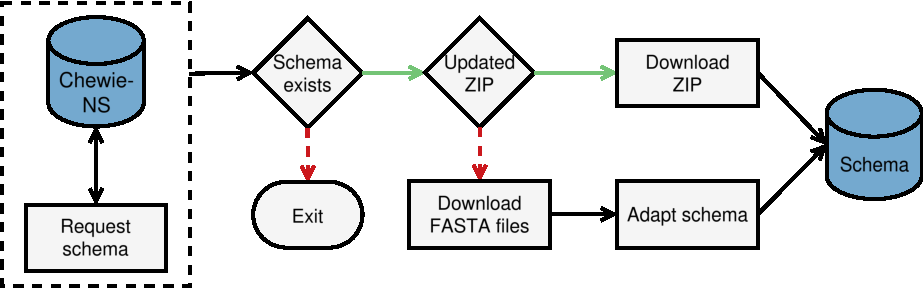
\includegraphics[angle=0,width=\textwidth]{figures/chapter 2/FigureS9.pdf}
    \caption{Diagram of the DownloadSchema module. The DownloadSchema module imports schemas from Chewie-NS. The process starts by sending a request with species and schema identifiers to Chewie-NS. If the schema exists, the process checks for a compressed and up-to-date version of the schema to download. If the compressed schema in Chewie-NS is for the latest version of the schema, the compressed schema is downloaded and uncompressed to get a ready-to-use schema. Otherwise, the process will send requests to retrieve the FASTA files with the alleles for all loci and determine the representative alleles with the PrepExternalSchema module to create the schema locally. Grey rectangle icons represent analysis steps. Diamond icons represent conditional statements, with green arrows used when the condition is met and red dashed arrows otherwise. The blue cylinder icons represent schemas.}
    \label{fig:chap2_figureS9}
\end{figure*}

\newpage
\begin{figure*}[h!]
    \centering
    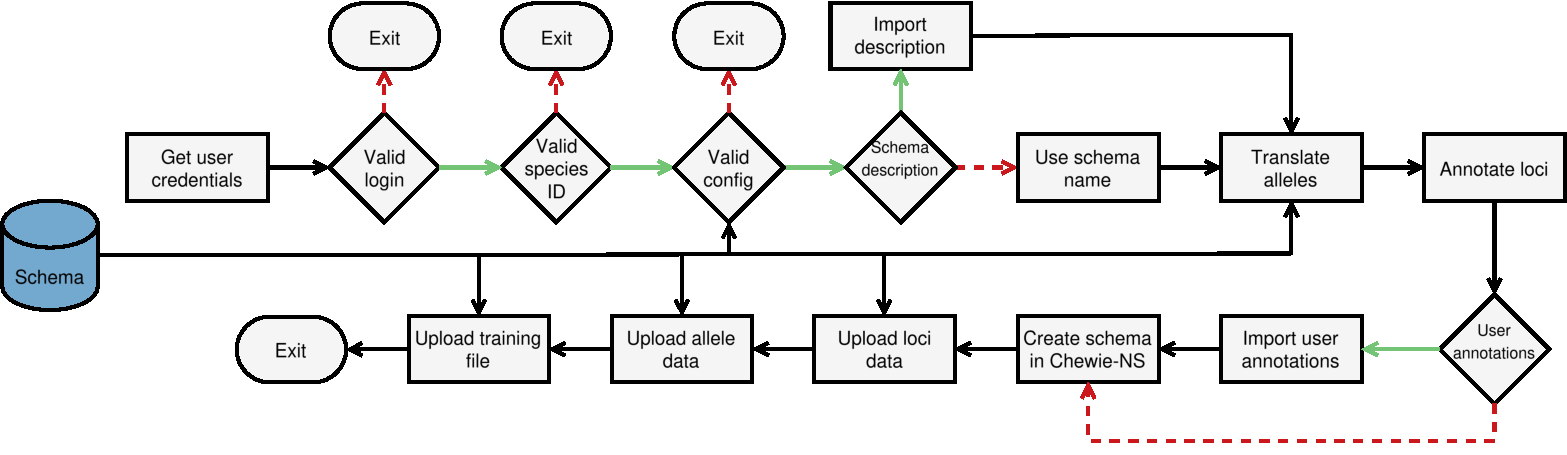
\includegraphics[angle=0,width=\textwidth]{figures/chapter 2/FigureS10.pdf}
    \caption{Diagram of the LoadSchema module. The LoadSchema module uploads local schemas to Chewie-NS. The process starts by requesting the user credentials to ensure that the user has contributor privileges. Only contributors are allowed to upload schemas to Chewie-NS. If the user is a contributor, the process checks if the species identifier provided by the user is valid and if the species is listed in Chewie-NS. After this step, the process reads the schema’s configuration file to validate the schema parameter values and ensure that there is only a single value associated with each parameter. The initial validation steps are followed by the upload of the schema data to Chewie-NS. The process reads the schema description, if the user provided one, or uses the schema name as description. The alleles are translated and annotation terms for the loci are obtained through UniProt’s SPARQL endpoint. If the user provides custom loci annotations, the process reads the file provided by the user and adds the custom annotations to the loci annotation data to send to Chewie-NS. After retrieving loci annotations, the process creates the schema in Chewie-NS by sending the schema’s parameter values and the list of file hashes to validate schema files uploaded in subsequent steps. The loci are created and linked to the newly created schema by sending the loci identifiers and annotations to Chewie-NS. The loci FASTA files are compressed and uploaded to Chewie-NS to add the allele sequences to the database and link them to the corresponding loci. The last step in the process uploads the training file in the local schema and associates it to the newly created schema in Chewie-NS. After process completion, Chewie-NS will process the data that was sent to make the schema data and statistics available through the website and the API. Grey rectangle icons represent analysis steps. Diamond icons represent conditional statements, with green arrows used when the condition is met and red dashed arrows otherwise. The blue cylinder icon represents a schema.}
    \label{fig:chap2_figureS10}
\end{figure*}

\newpage
\begin{figure*}[h!]
    \centering
    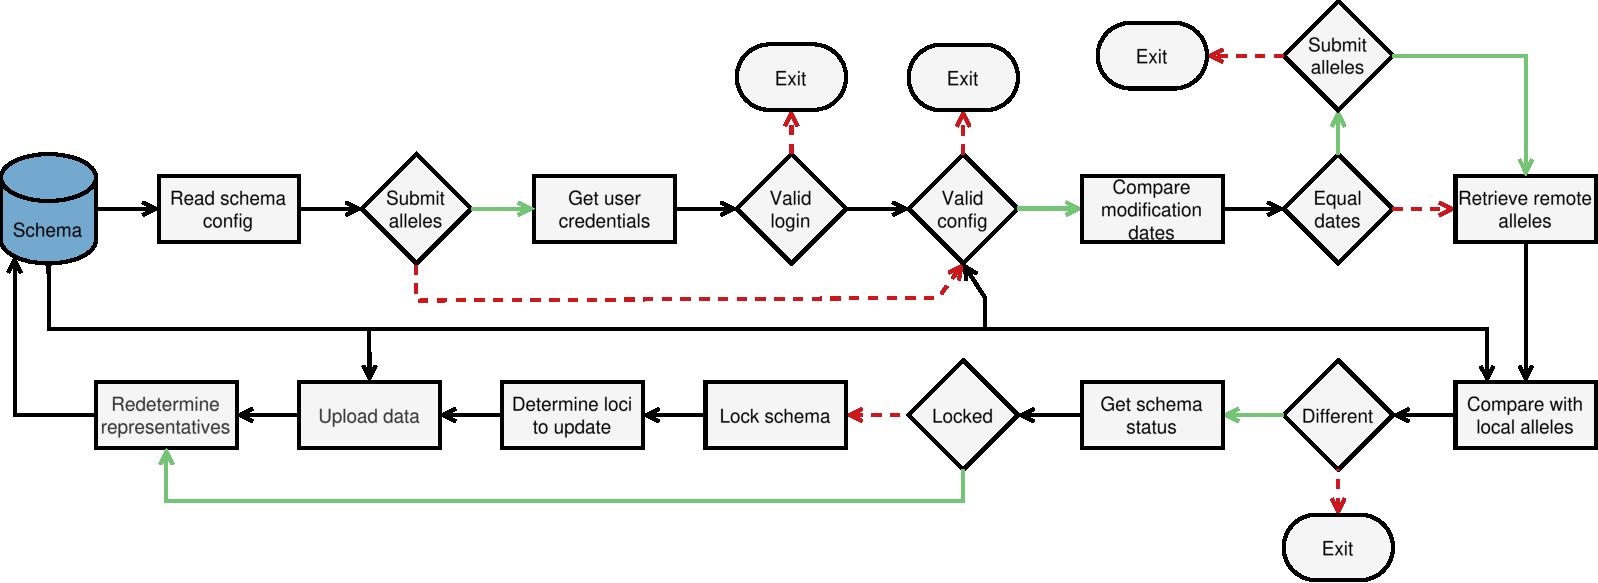
\includegraphics[angle=0,width=\textwidth]{figures/chapter 2/FigureS11.pdf}
    \caption{Diagram of the SyncSchema module. The SyncSchema module retrieves new alleles added to remote schemas in Chewie-NS and submits new alleles added to local schemas to update the remote schemas in Chewie-NS. The process starts by reading the schema’s configuration file to get the schema’s parameter values and ensure the values match the ones listed in Chewie-NS. If the user wants to submit new alleles identified locally (--submit), the process will ask for the user credentials to verify if the user has contributor privileges. Before retrieving or uploading new alleles, the process verifies if the last modification date of the local and remote schemas match. If the dates match and the user does not want to submit new local alleles, the process exits. If the dates do not match or the user wants to submit new local alleles, the process retrieves new alleles added to the remote schema since the last modification date and compares them with the alleles in the local schema. If any alleles are exclusive to the local or remote schema, the process creates updated FASTA files with all the alleles and locks the remote schema to ensure that only the current user can modify the remote schema. The process creates files with the data for the new local alleles and sends them to Chewie-NS, waiting for Chewie-NS to insert the new alleles into the database. After allele insertion in Chewie-NS, the process adapts the updated FASTA files with the PrepExternalSchema module to update the local schema and ensure that the local and remote allele identifiers match. If the schema was already locked by another user, the process will skip data upload to Chewie-NS and will update the local schema with new alleles retrieved from Chewie-NS. Grey rectangle icons represent analysis steps. Diamond icons represent conditional statements, with green arrows used when the condition is met and red dashed arrows otherwise. The blue cylinder icon represents a schema.}
    \label{fig:chap2_figureS11}
\end{figure*}

\newpage
\begin{figure*}[h!]
    \centering
    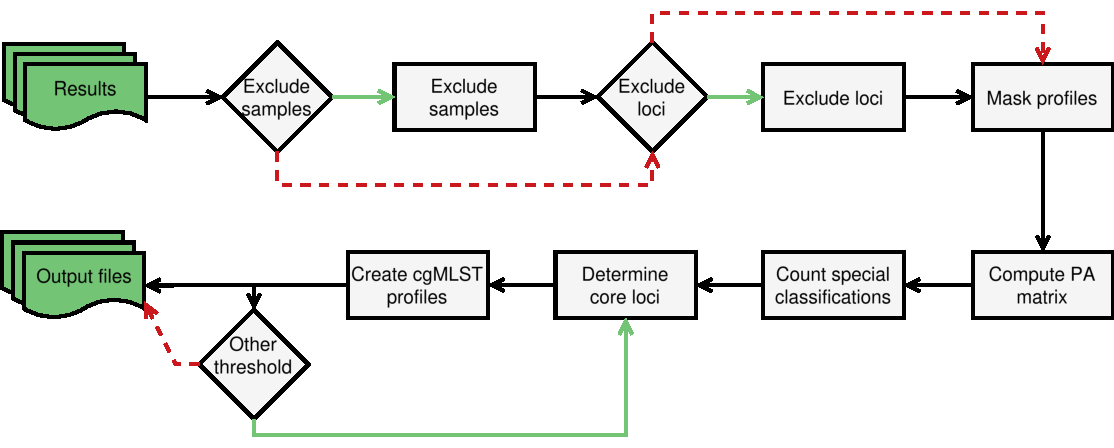
\includegraphics[angle=0,width=\textwidth]{figures/chapter 2/FigureS12.pdf}
    \caption{Diagram of the ExtractCgMLST module. The ExtractCgMLST module determines the set of core loci based on the allelic profiles determined by the AlleleCall module. The process starts by excluding loci and samples from the analysis based on lists of loci and samples provided by the user. This allows users to filter out low-quality samples and problematic loci that would affect the determination of the core genome. The filtered allelic profiles are masked to remove the INF- prefixes from newly inferred alleles and substitute special classifications by 0. The masked profiles are used to compute a loci presence-absence matrix and count the number of special classifications per sample. The presence-absence matrix is also used to determine the set of core loci based on the default loci presence thresholds of 0.9, 0.95 and 1, or based on threshold values specified by the user. The process creates output files with the list of loci and allelic profiles per threshold and creates an HTML file with a scatter plot representing the core genome size variation for each threshold. The green document icons represent input and output files. Grey rectangle icons represent analysis steps. Diamond icons represent conditional statements, with green arrows used when the condition is met and red dashed arrows otherwise.}
    \label{fig:chap2_figureS12}
\end{figure*}

\newpage
\begin{figure*}[h!]
    \centering
    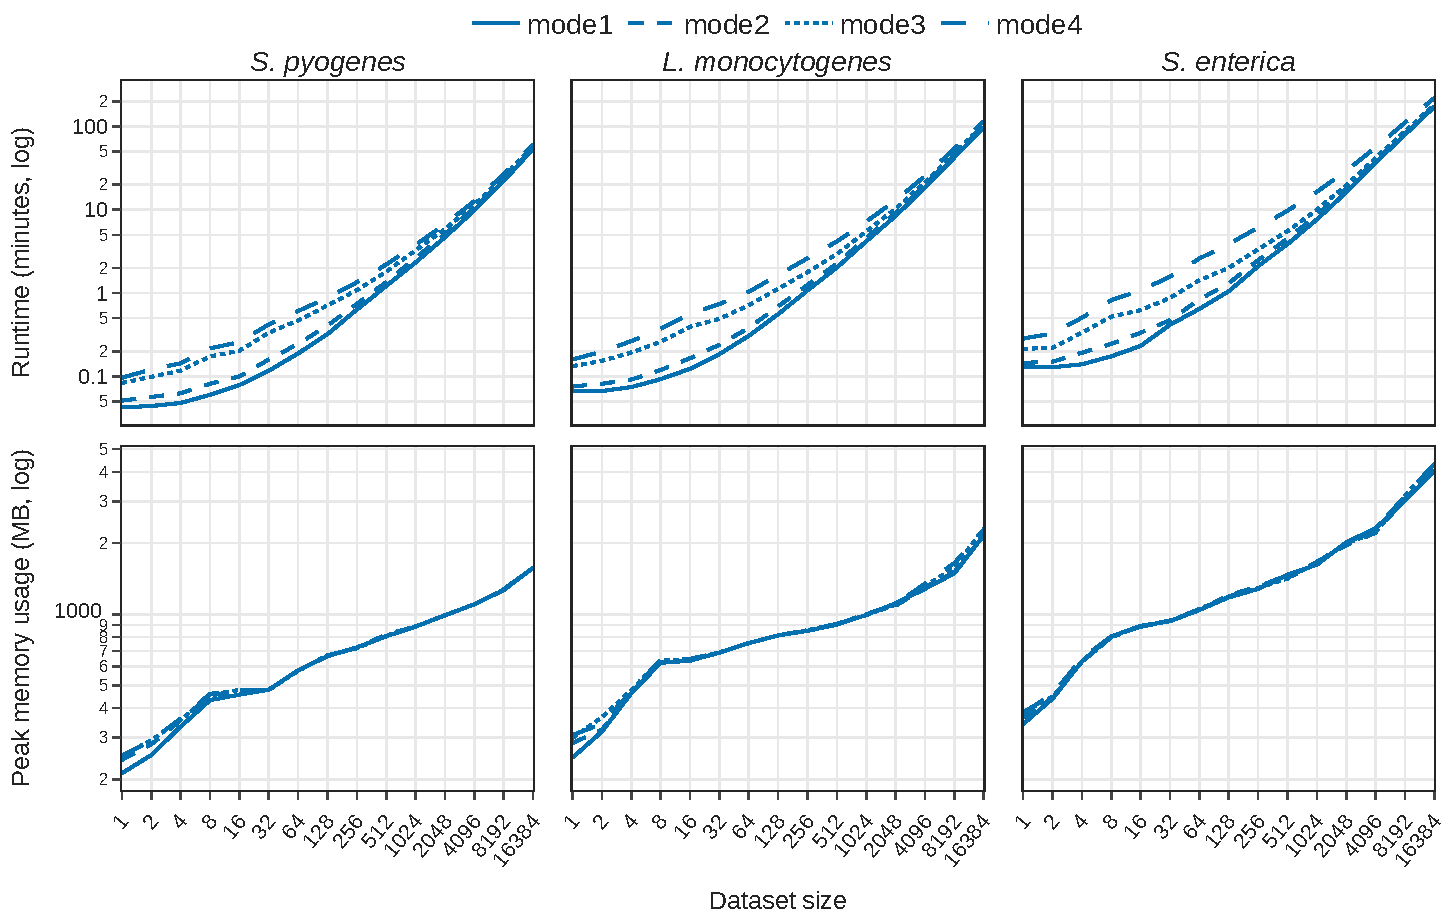
\includegraphics[angle=0,width=\textwidth]{figures/chapter 2/FigureS13.pdf}
    \caption{Runtime and peak memory usage for the four execution modes available in chewBBACA 3. Runtime and peak memory usage were measured for the allele calling of datasets with 1 to 16384 strains for three bacterial species: Streptococcus pyogenes, Listeria monocytogenes, and Salmonella enterica. The benchmark was performed with five replicates per dataset size, except for the complete dataset (n=16,384 genomes). The values shown are the mean of the replicate values for each dataset. Runtime was measured as the elapsed real time in minutes (logarithmic scale). Peak memory usage was measured as the maximum resident set size in MB (logarithmic scale).}
    \label{fig:chap2_figureS13}
\end{figure*}

\newpage
\begin{figure*}[h!]
    \centering
    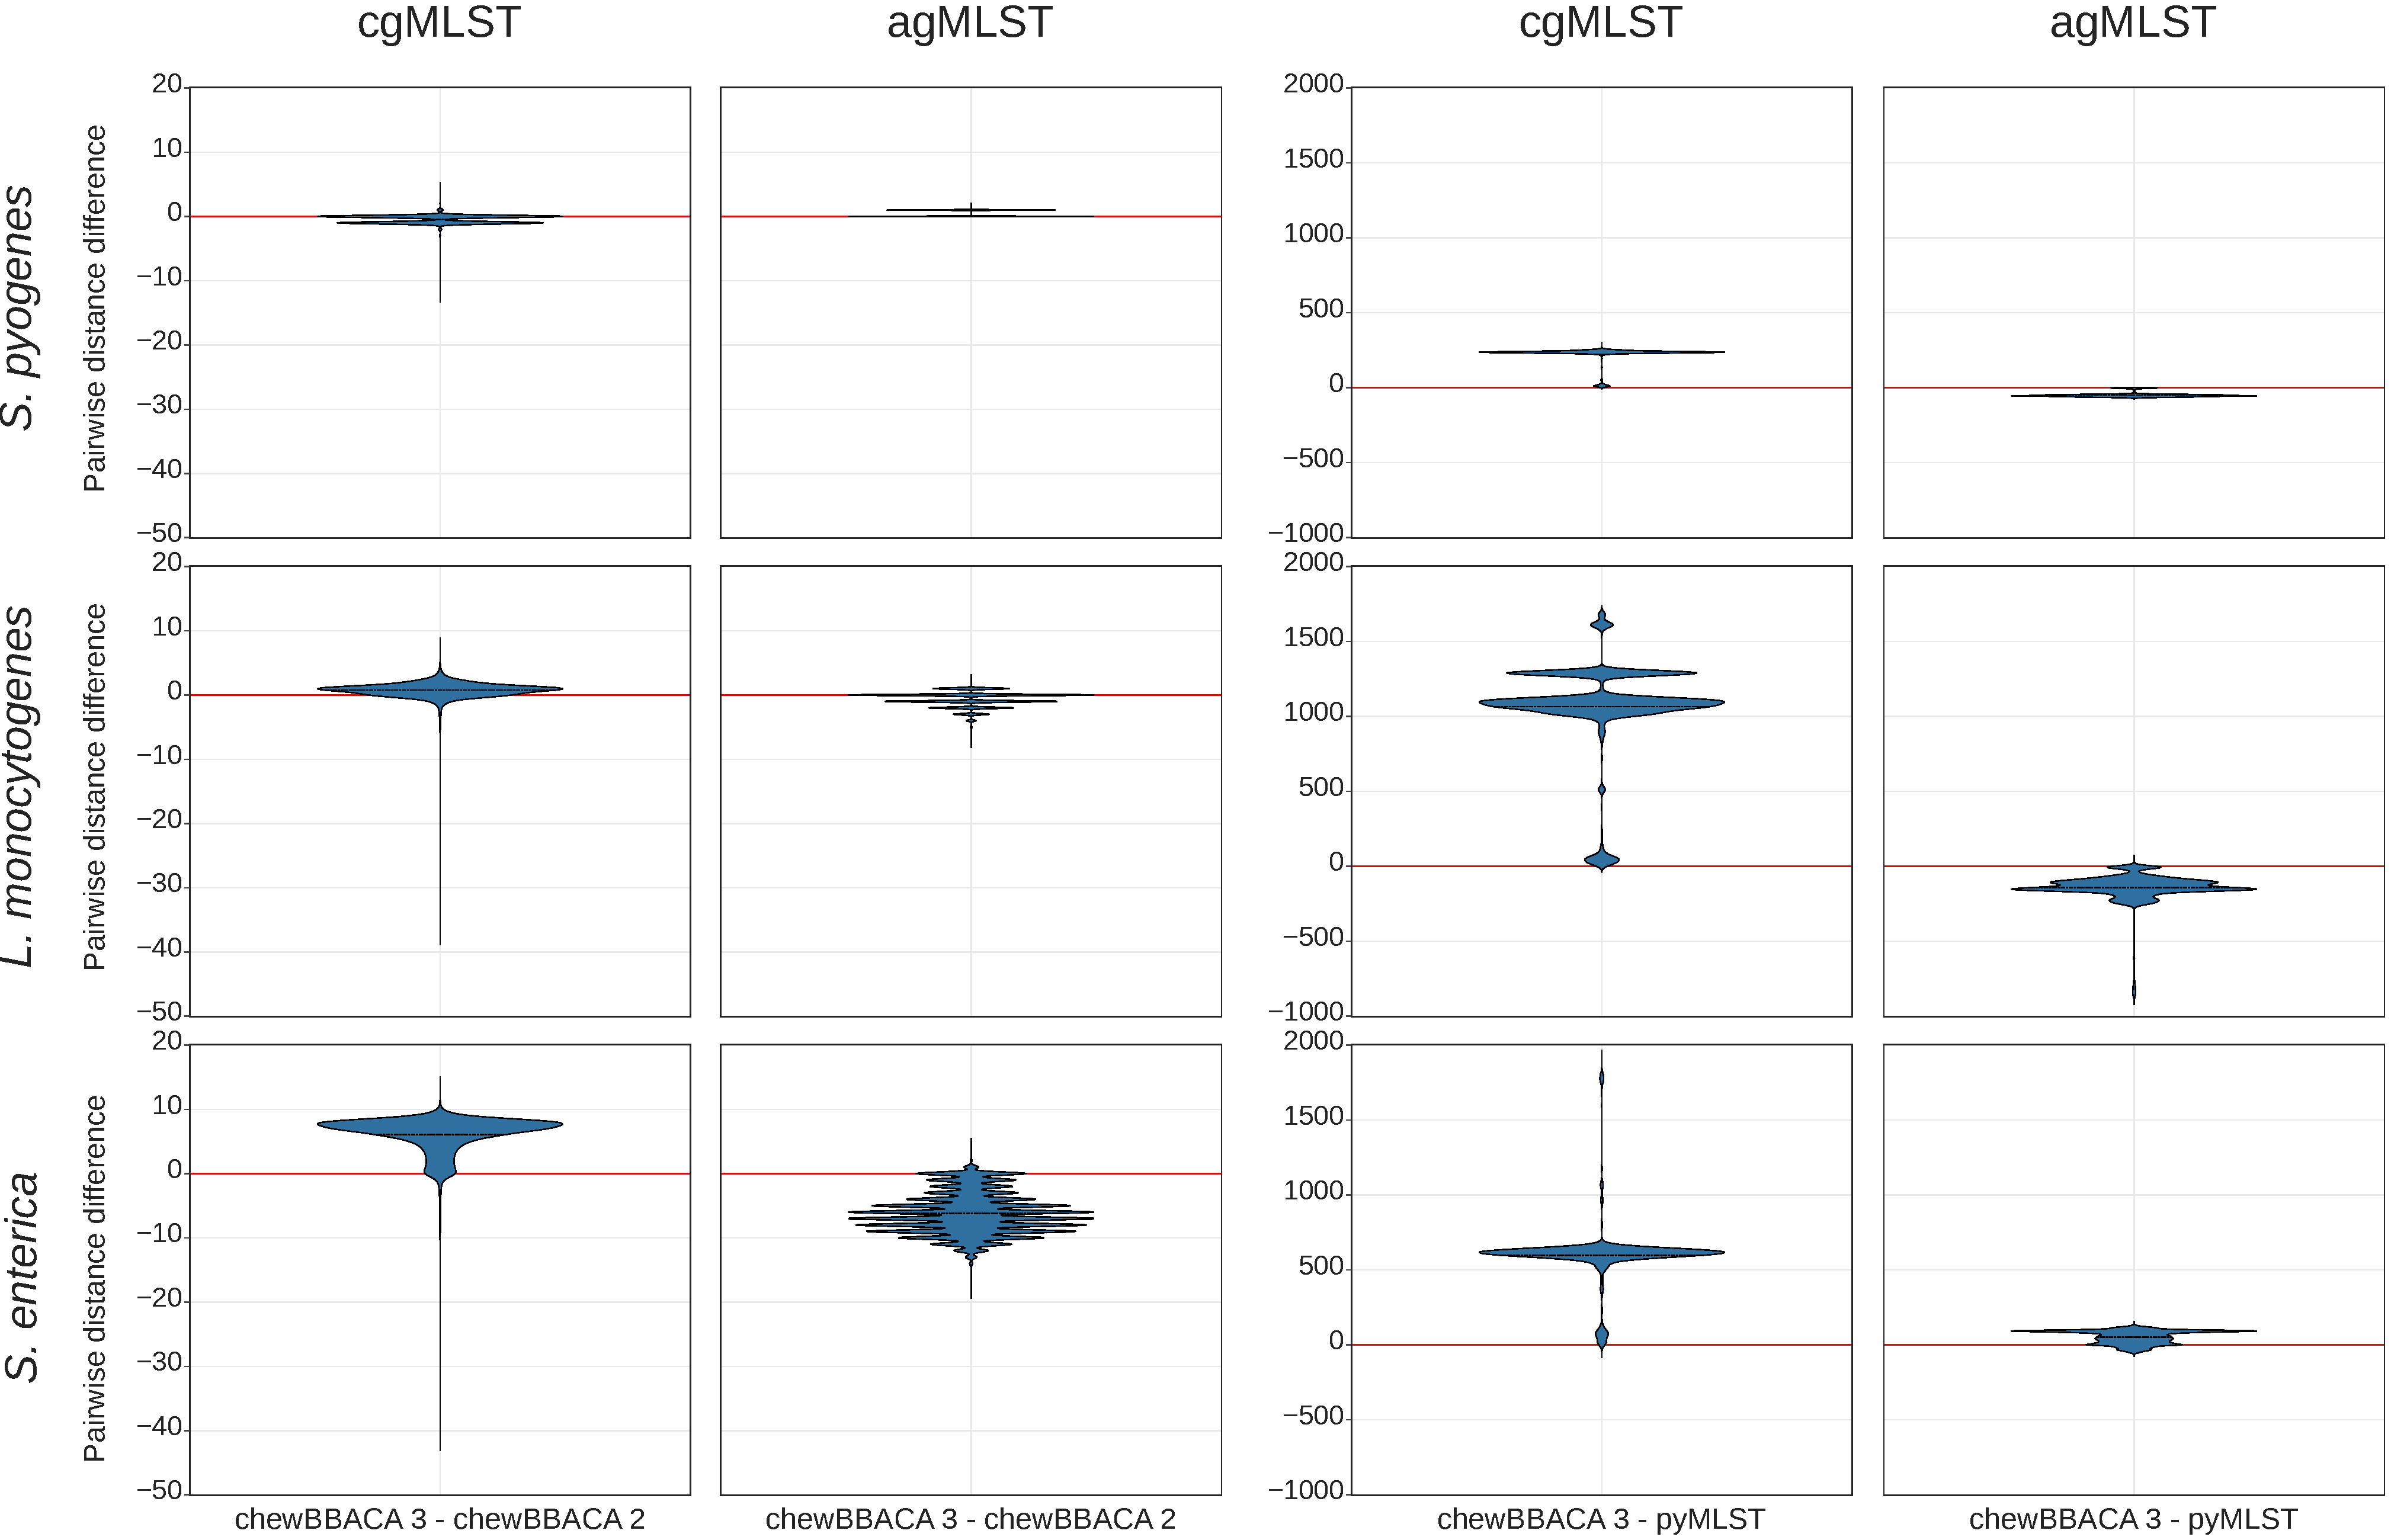
\includegraphics[angle=0,width=\textwidth]{figures/chapter 2/FigureS14.pdf}
    \caption{Pairwise allelic distances differences. The pairwise distances differences at the core-genome (cgMLST) and accessory-genome (agMLST) levels were computed by subtracting the allelic distance matrices computed based on chewBBACA 2's and pyMLST's results from the allelic distance matrices computed from chewBBACA 3's results for the complete datasets (n=16,384 genomes). A positive value represents a greater difference with chewBBACA 3 and a negative value a smaller difference with chewBBACA 3 than with the comparator. The zero line in each plot is highlighted in red.}
    \label{fig:chap2_figureS14}
\end{figure*}

\newpage
\begin{figure*}[h!]
    \centering
    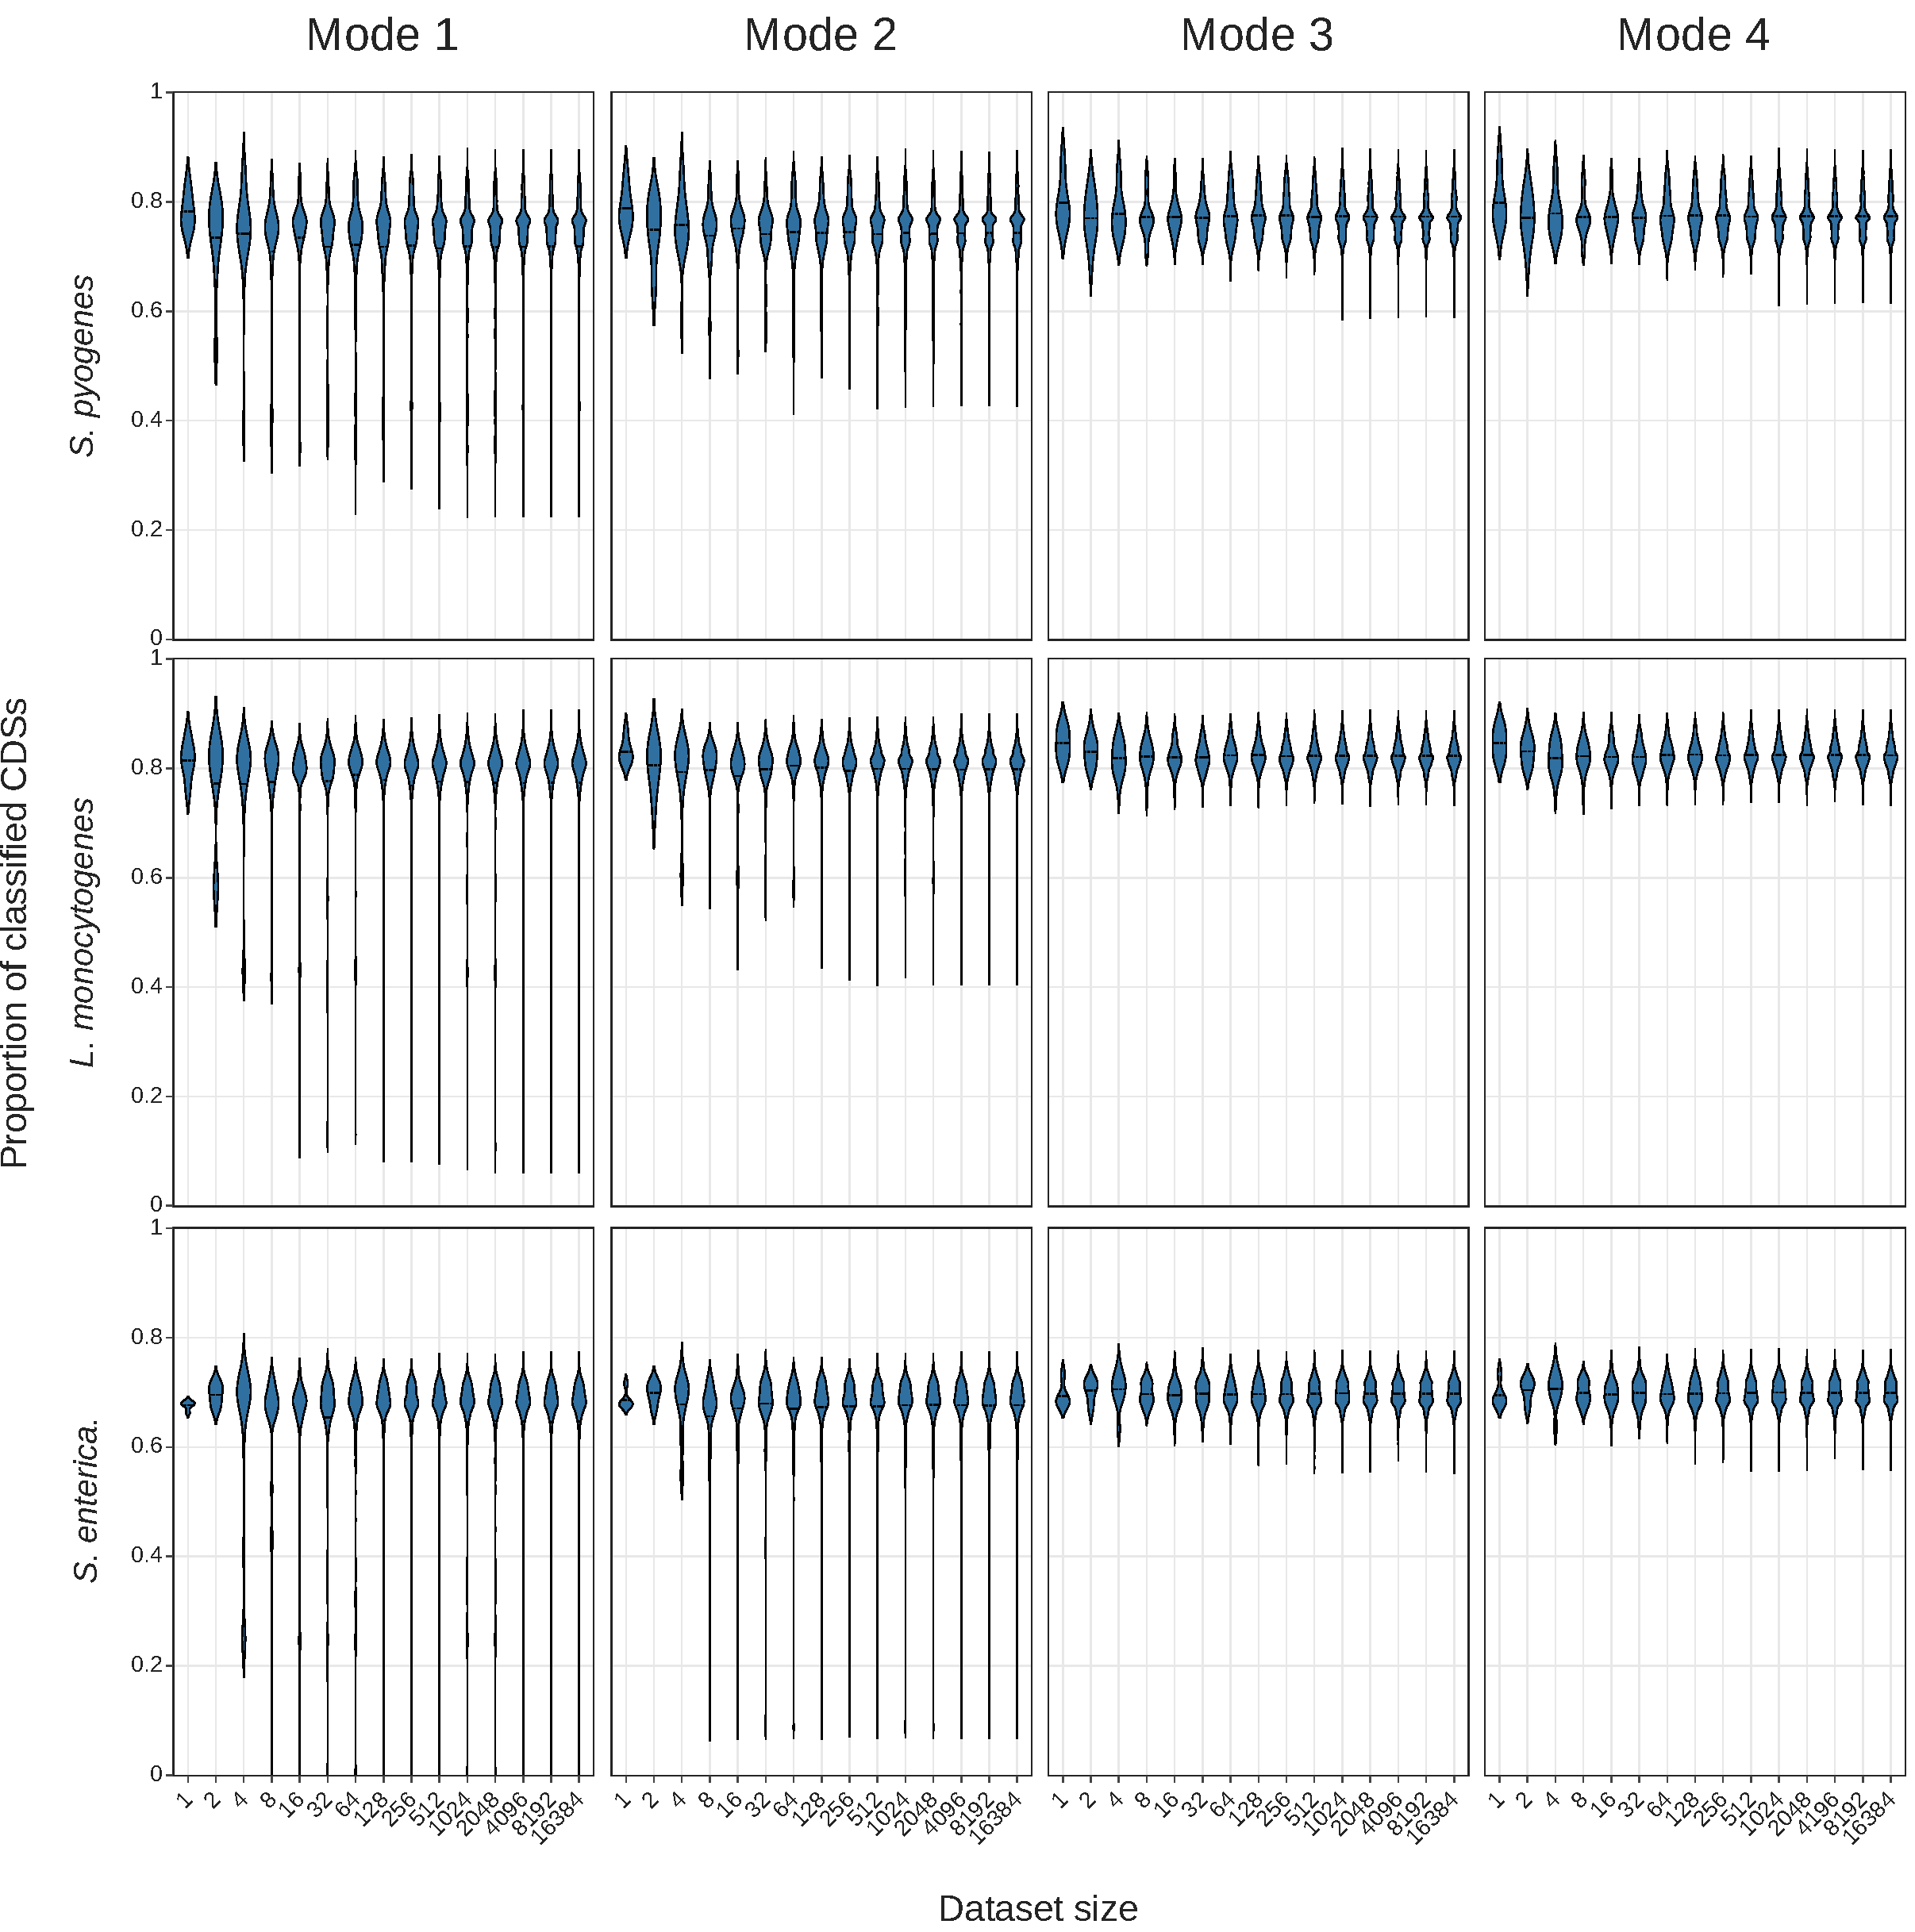
\includegraphics[angle=0,width=\textwidth]{figures/chapter 2/FigureS15.pdf}
    \caption{Proportion of CDSs classified per execution mode for each species’ datasets. The proportion of classified CDSs corresponds to the number of CDSs classified by each execution mode divided by the total number of CDSs predicted for each strain by Pyrodigal. The benchmark was performed with five replicates per dataset size, except for the complete dataset (n=16,384 genomes).}
    \label{fig:chap2_figureS15}
\end{figure*}

\newpage
\begin{figure*}[h!]
    \centering
    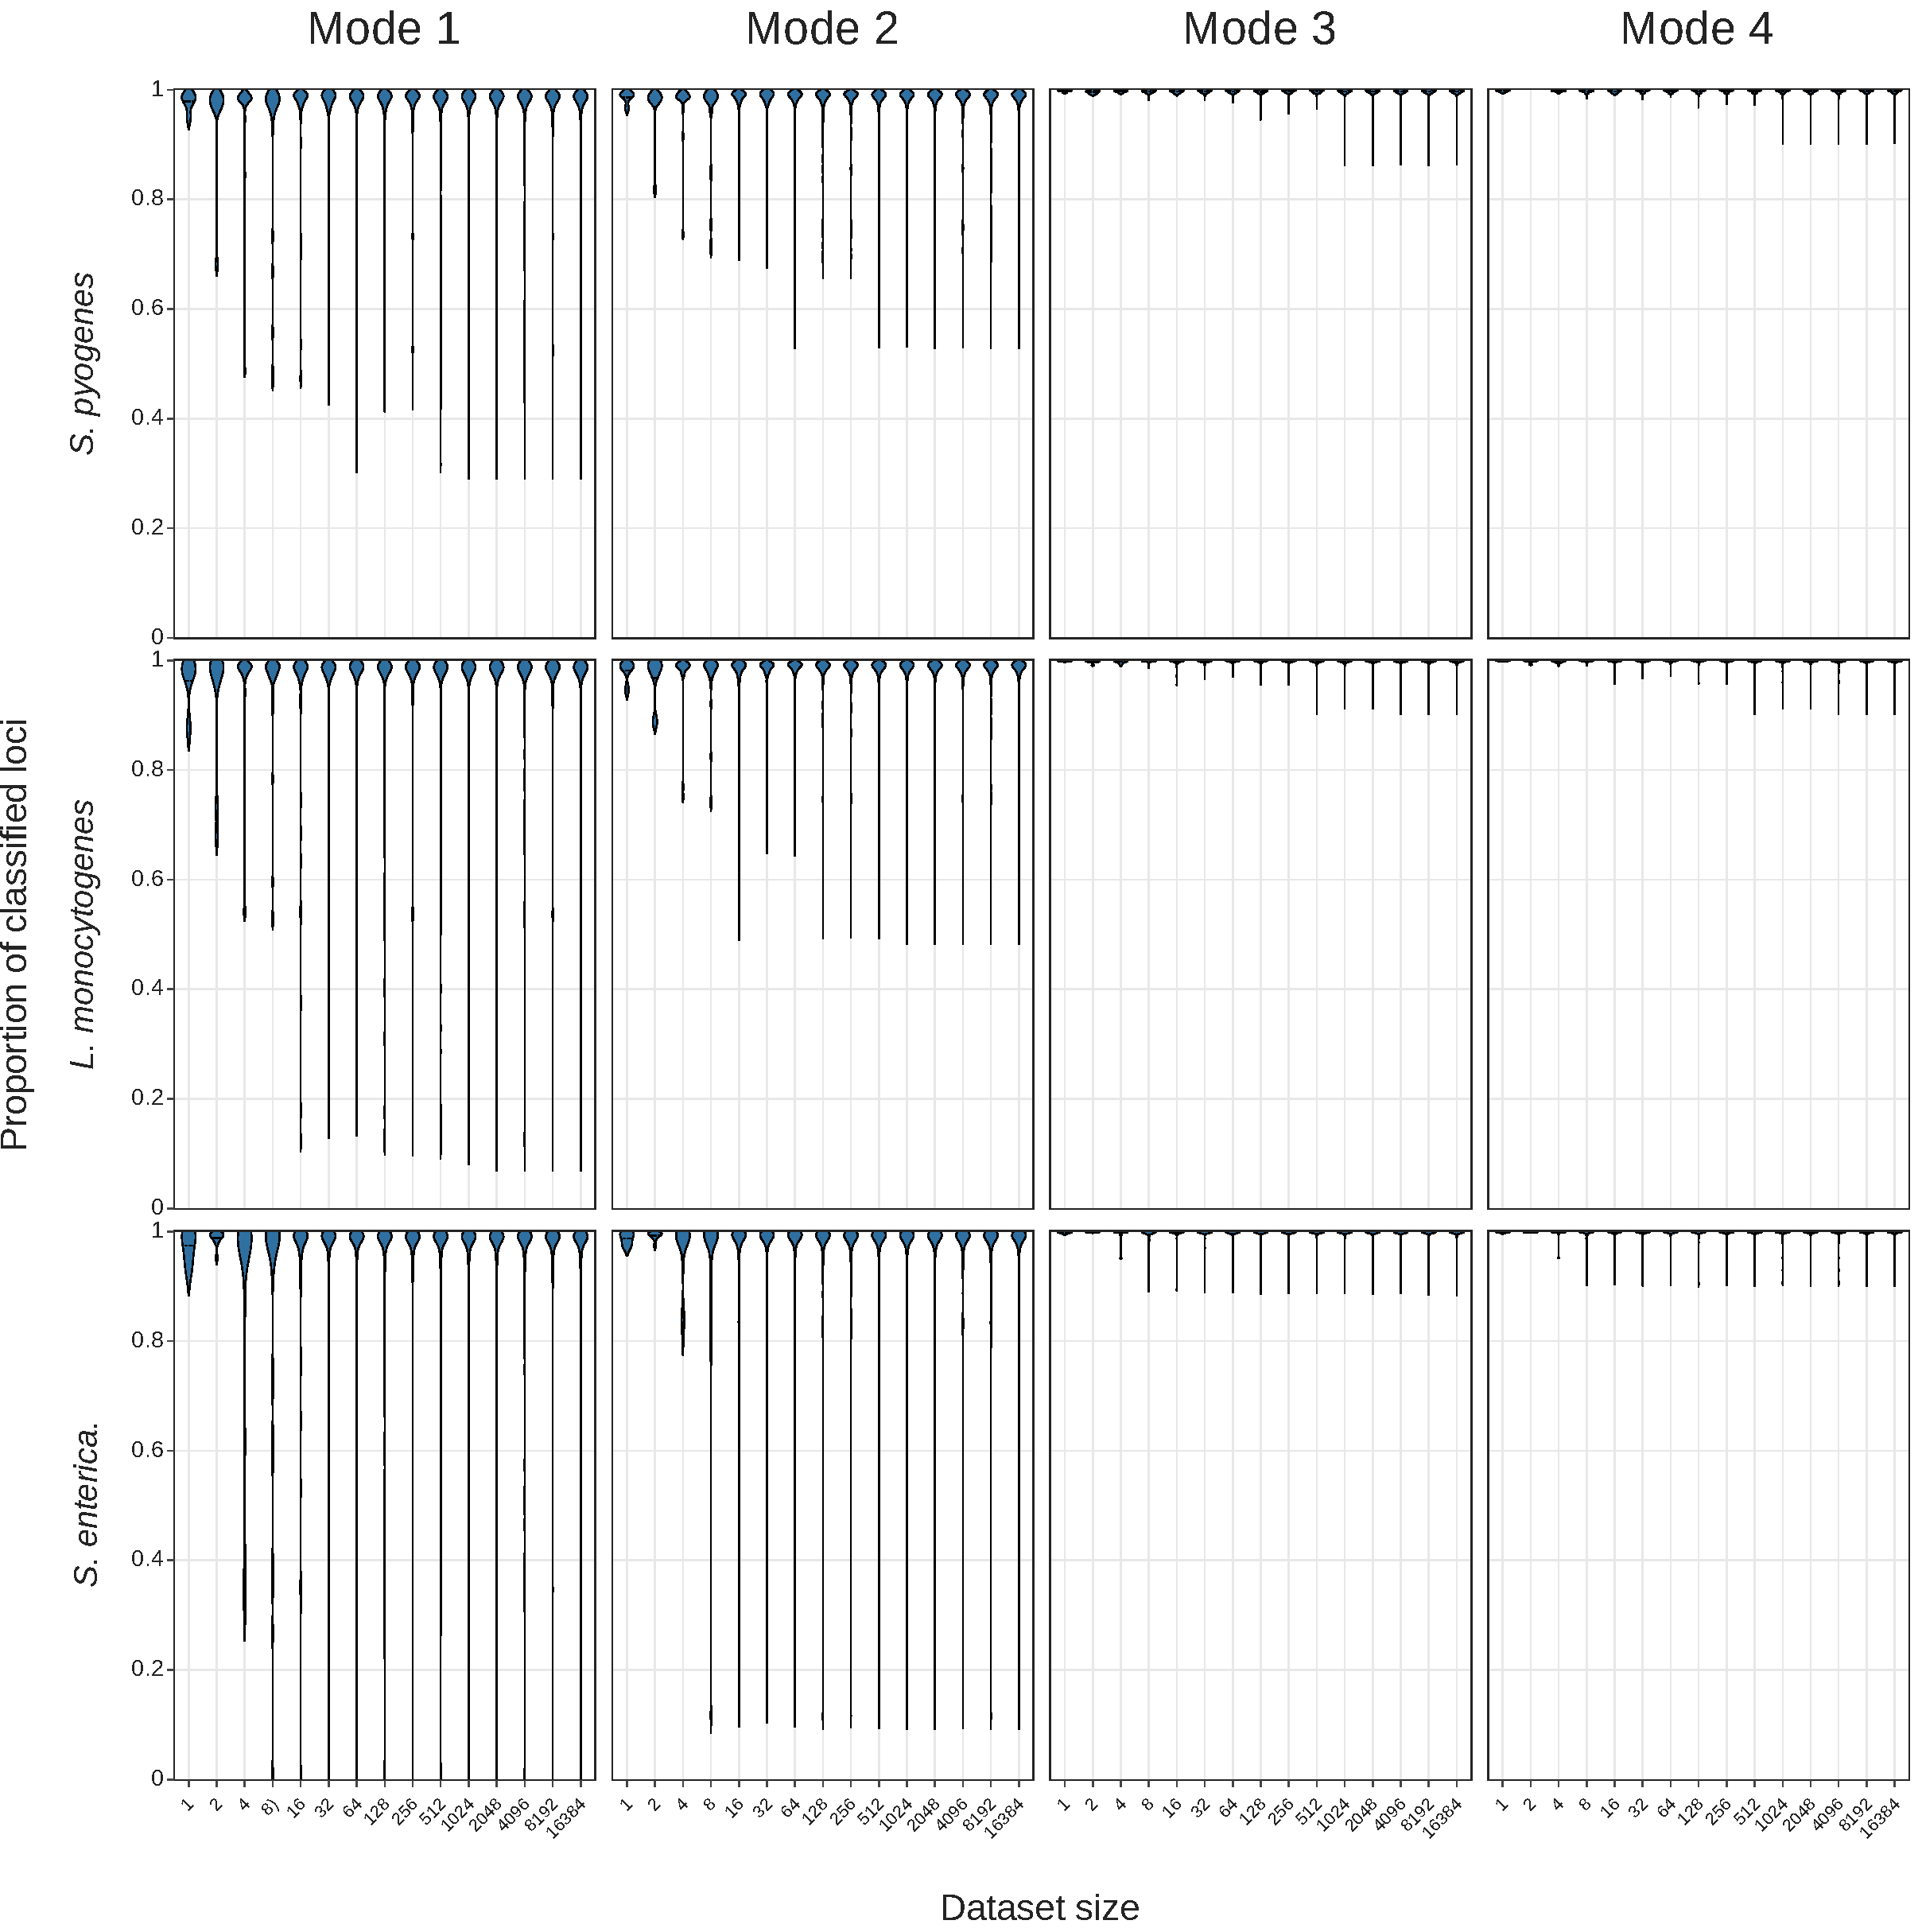
\includegraphics[angle=0,width=\textwidth]{figures/chapter 2/FigureS16.pdf}
    \caption{Proportion of schema loci classified per execution mode for each species’ datasets. The proportion of classified loci corresponds to the number of schema loci identified by each execution mode divided by the total number of schema loci. The benchmark was performed with five replicates per dataset size, except for the complete dataset (n=16,384 genomes).}
    \label{fig:chap2_figureS16}
\end{figure*}

\newpage
\begin{figure*}[h!]
    \centering
    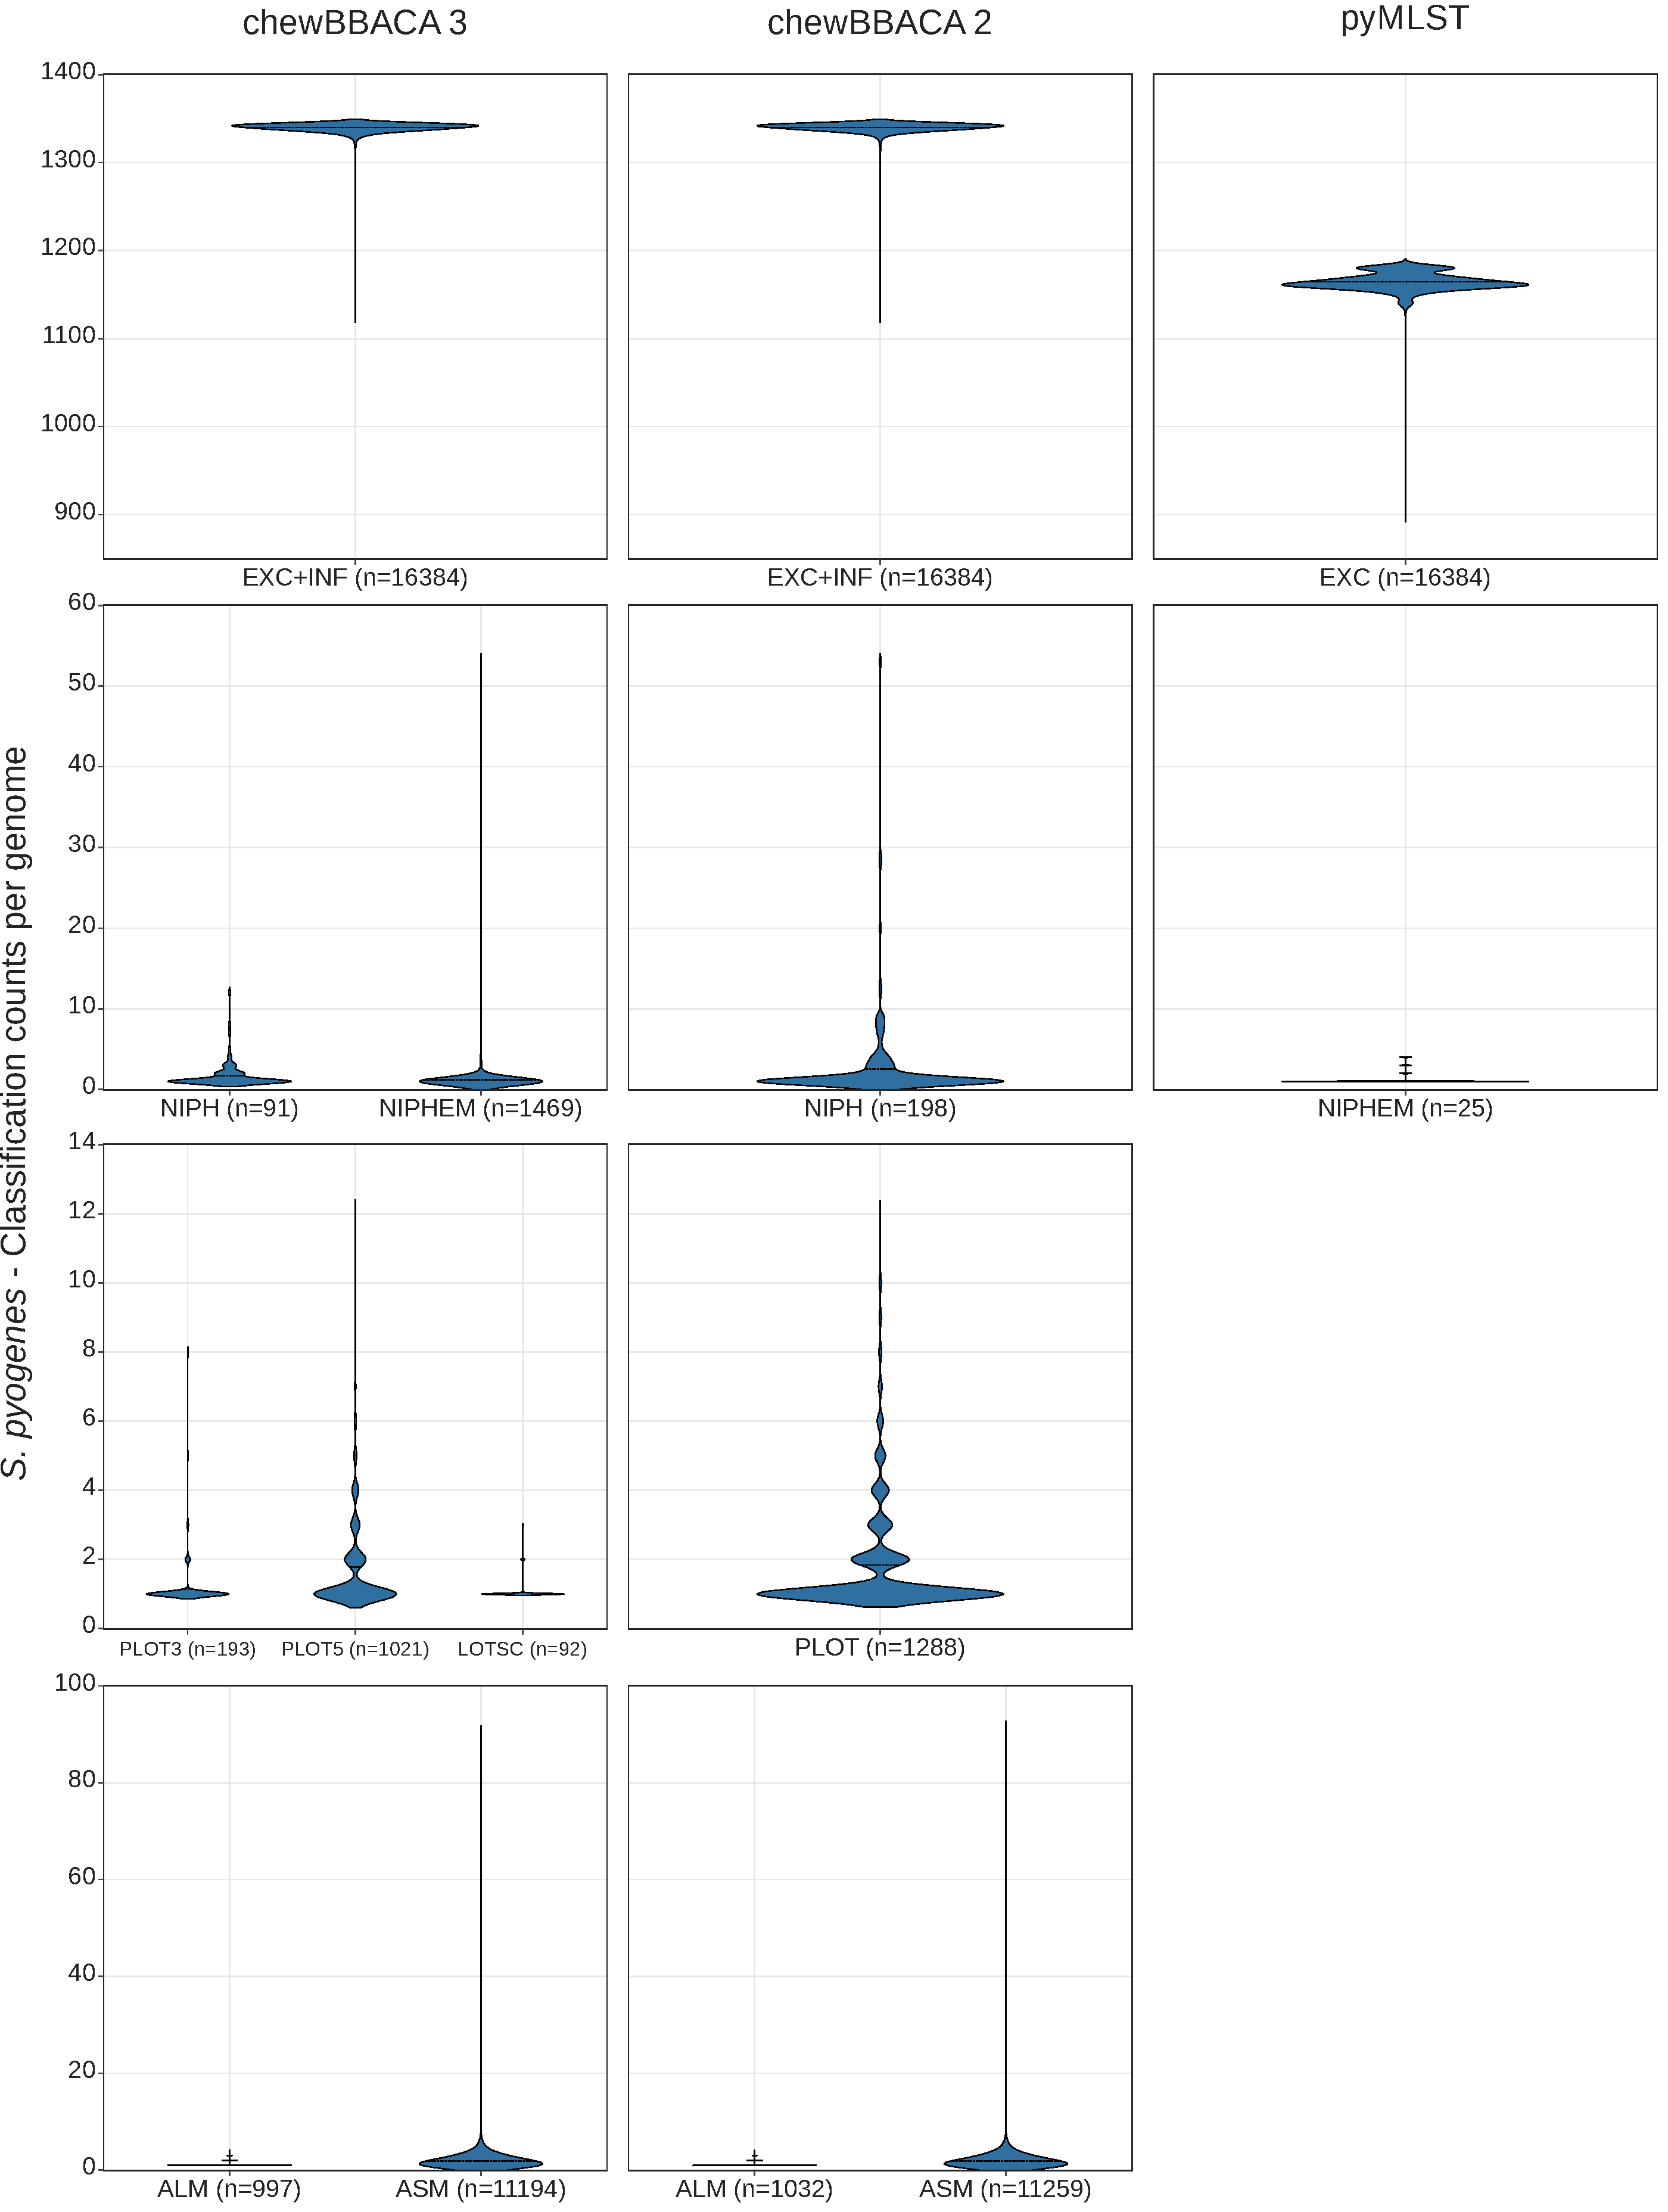
\includegraphics[angle=0,width=\textwidth]{figures/chapter 2/FigureS17.pdf}
    \caption{Classifications counts for the complete dataset (n=16,384 genomes) of S. pyogenes per tool. Each row displays the counts for the special classifications that are equivalent between tools. The x-axis labels show the names of the classifications and the number of genomes with a count above zero inside the parentheses (i.e. genomes with a count of zero for any of the classifications are not included in the plotted values). For pyMLST, the loci with a single matching CDS were converted to EXC and the loci with multiple matches were converted to NIPHEM. The plot is not shown if the tool does not determine a special classification equivalent to the ones displayed in the row.}
    \label{fig:chap2_figureS17}
\end{figure*}

\newpage
\begin{figure*}[h!]
    \centering
    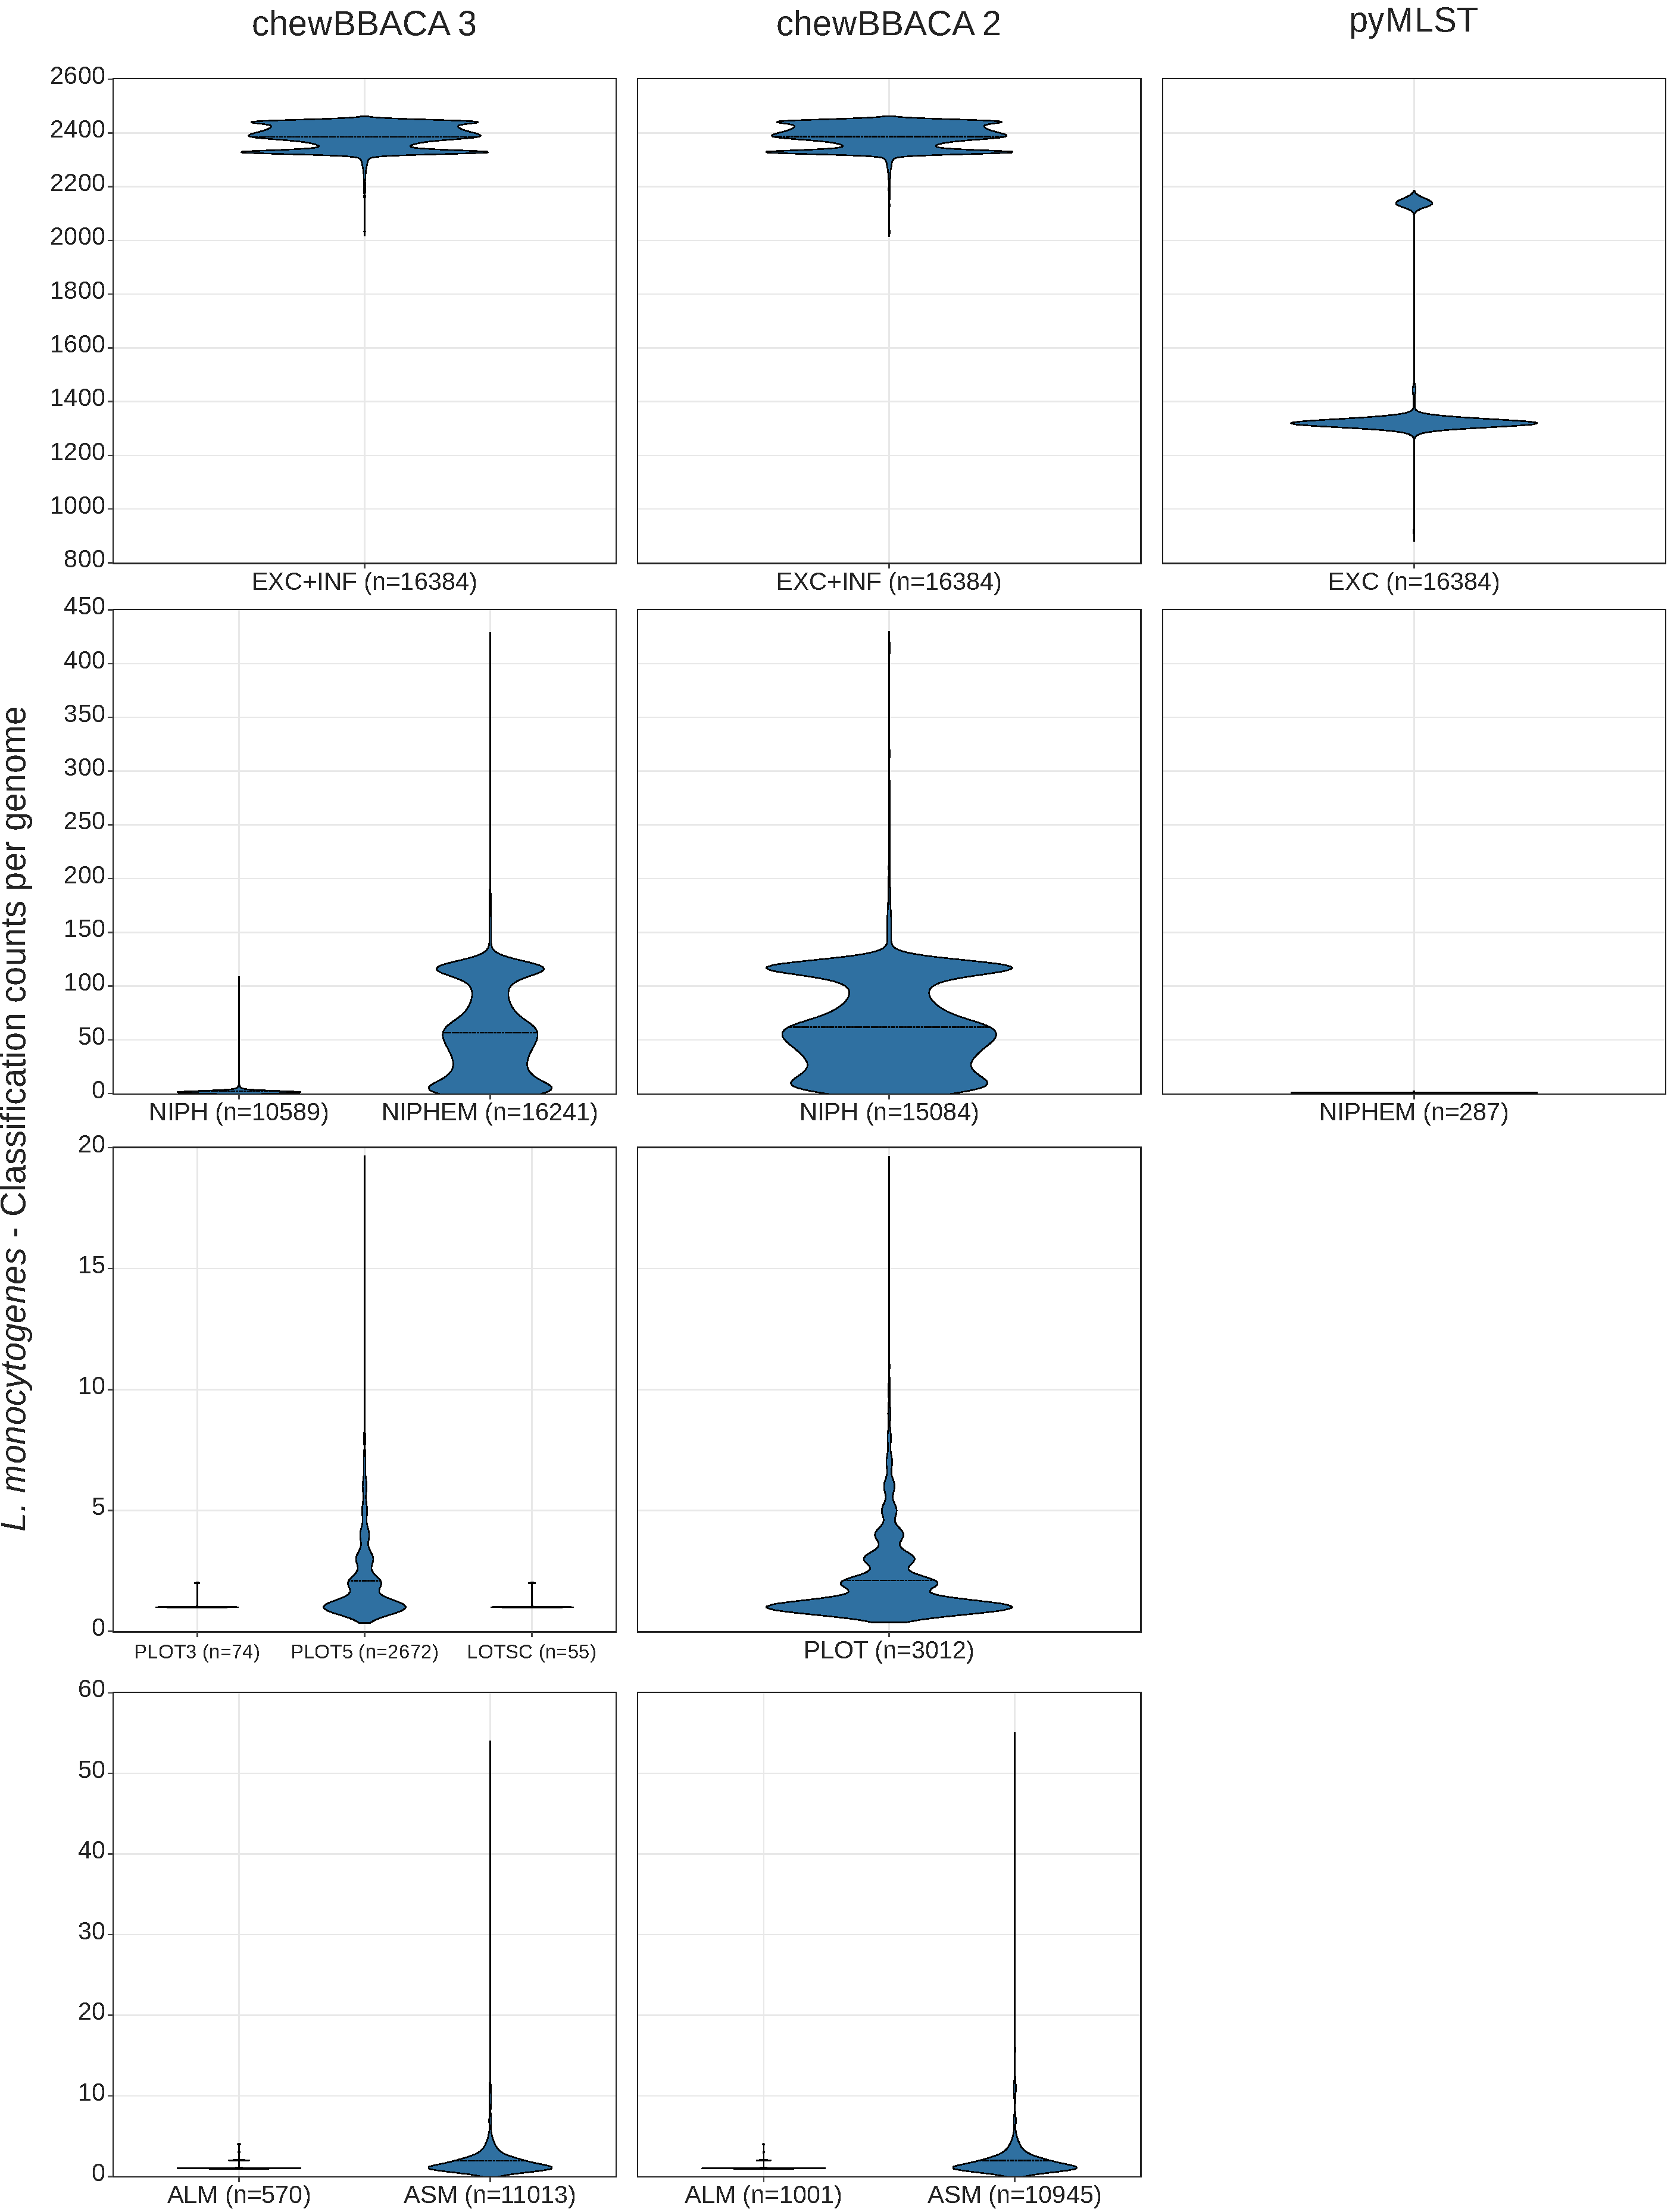
\includegraphics[angle=0,width=\textwidth]{figures/chapter 2/FigureS18.pdf}
    \caption{Classifications counts for the complete dataset (n=16,384 genomes) of L. monocytogenes per tool. Each row displays the counts for the special classifications that are equivalent between tools. The x-axis labels show the names of the classifications and the number of genomes with a count above zero inside the parentheses (i.e. genomes with a count of zero for any of the classifications are not included in the plotted values). For pyMLST, the loci with a single matching CDS were converted to EXC and the loci with multiple matches were converted to NIPHEM. The plot is not shown if the tool does not determine a special classification equivalent to the ones displayed in the row.}
    \label{fig:chap2_figureS18}
\end{figure*}

\newpage
\begin{figure*}[h!]
    \centering
    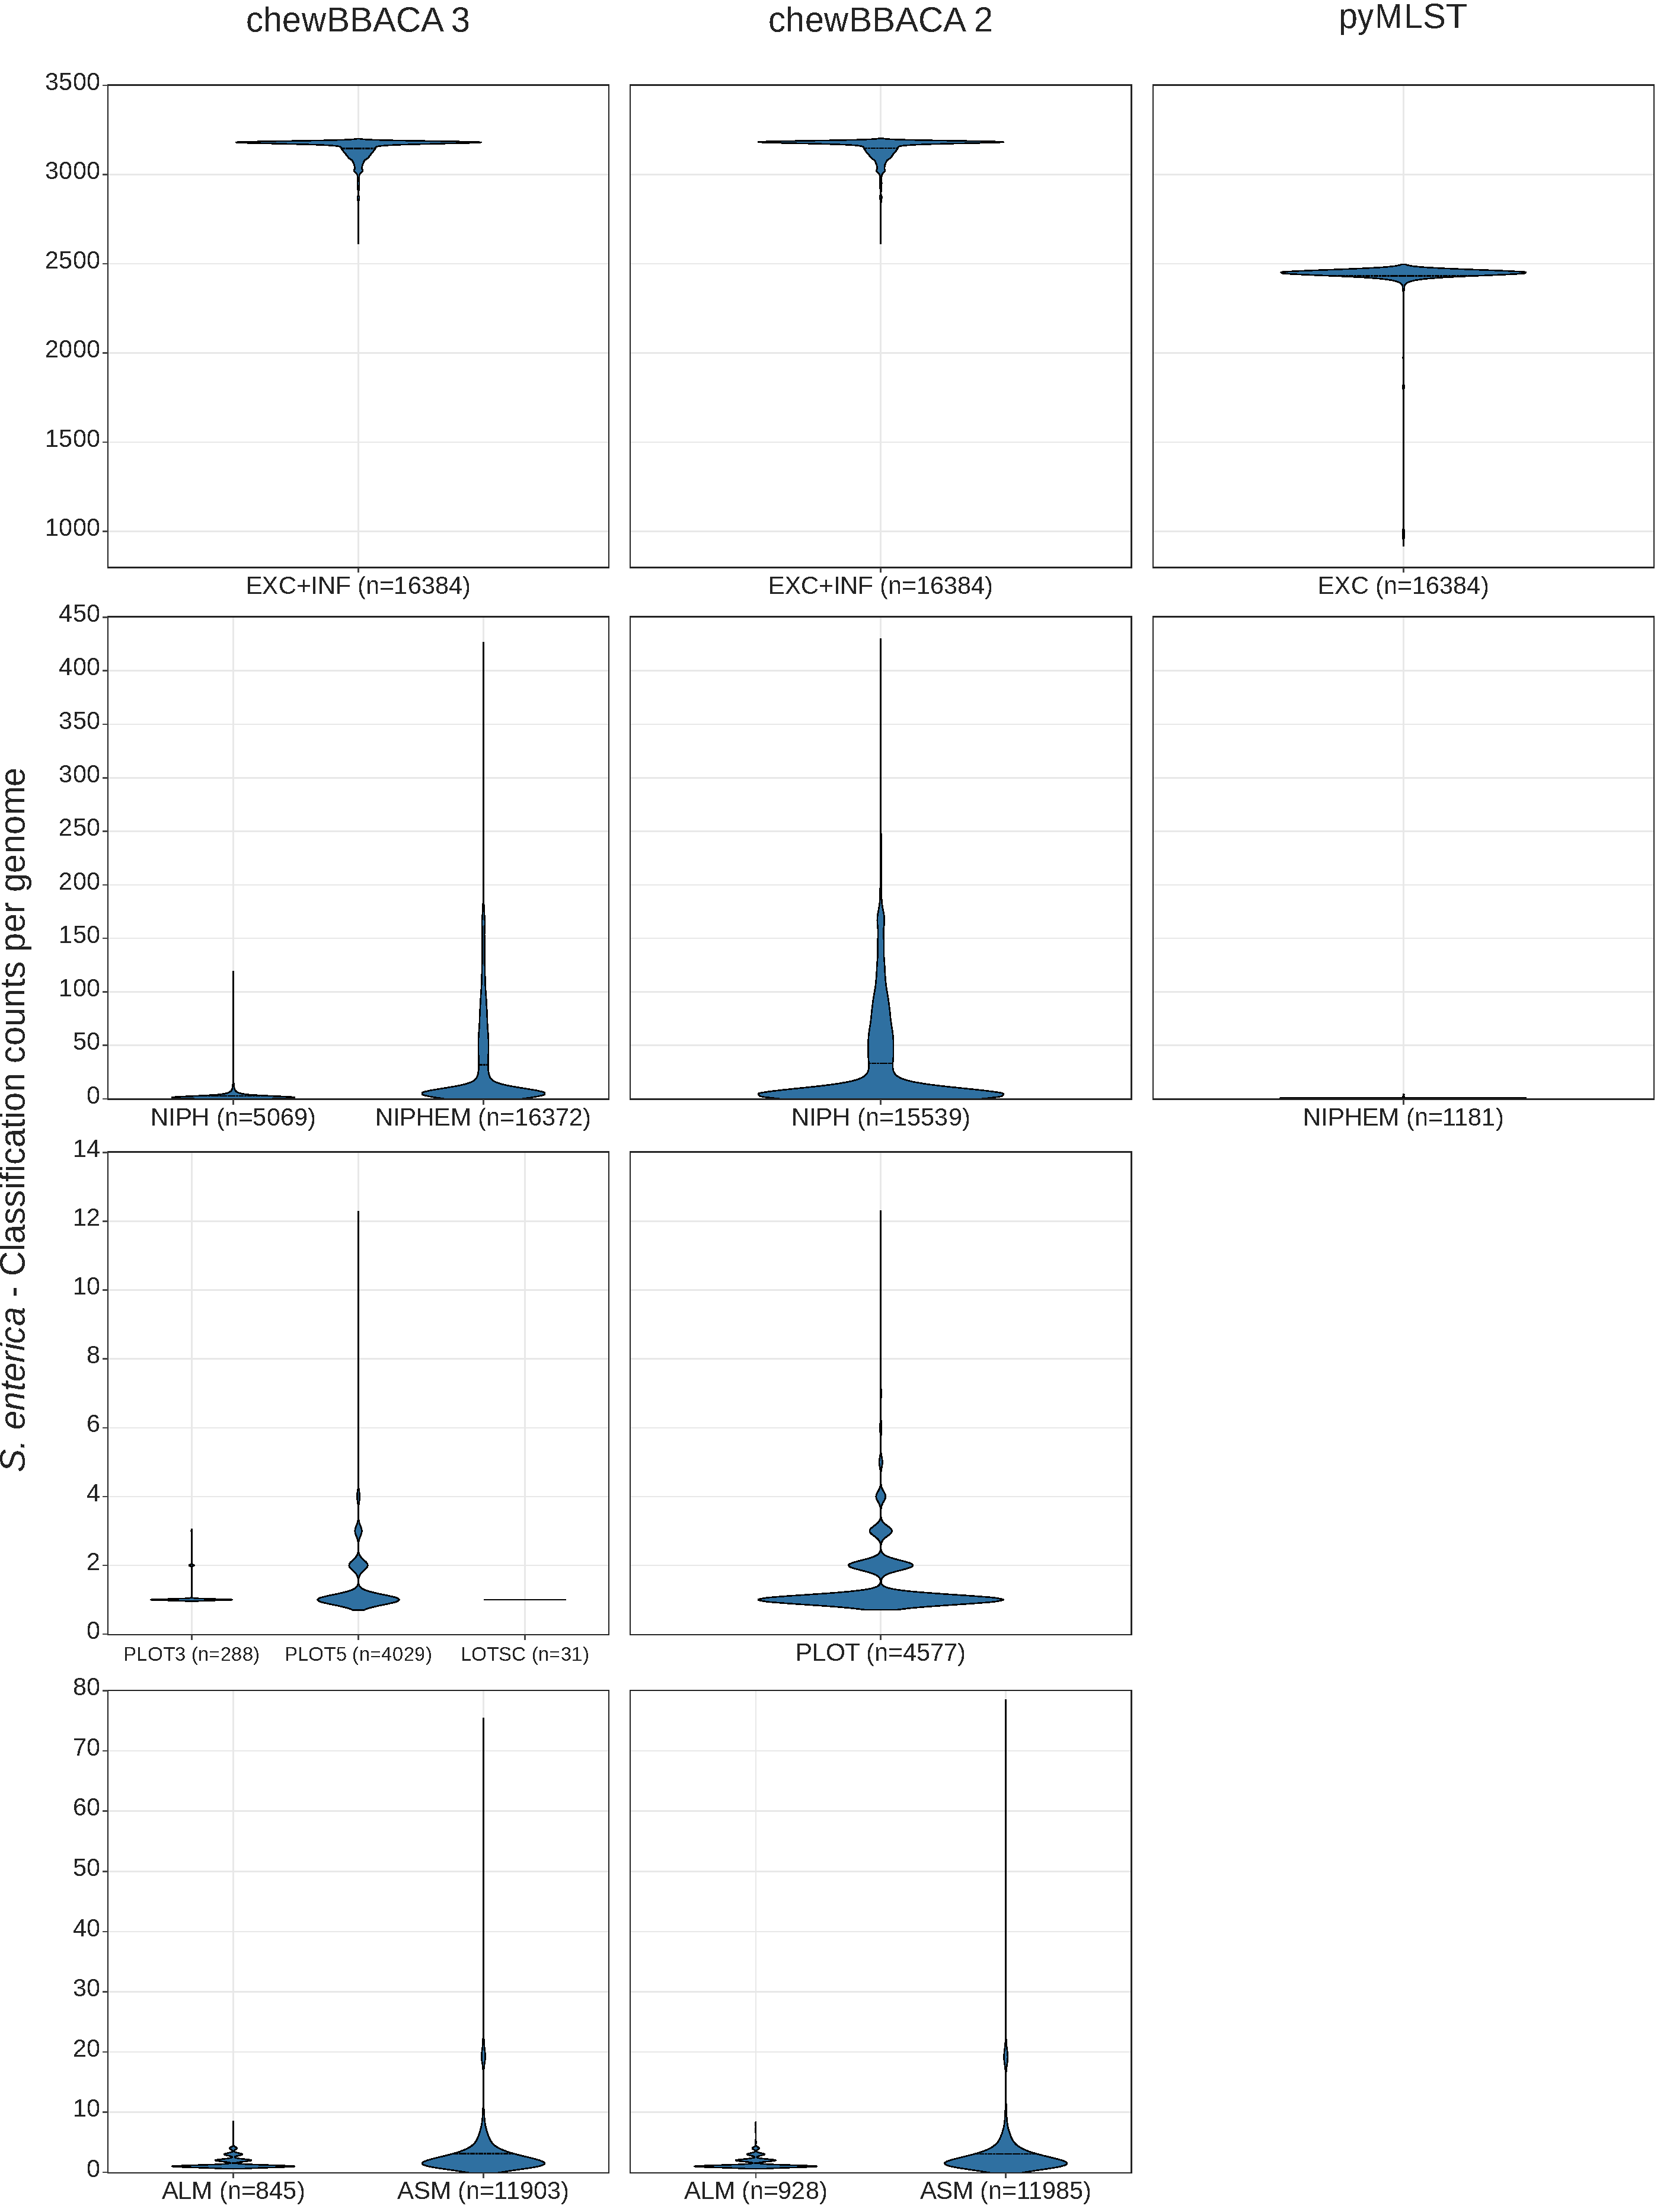
\includegraphics[angle=0,width=\textwidth]{figures/chapter 2/FigureS19.pdf}
    \caption{Classifications counts for the complete dataset (n=16,384 genomes) of S. enterica per tool. Each row displays the counts for the special classifications that are equivalent between tools. The x-axis labels show the names of the classifications and the number of genomes with a count above zero inside the parentheses (i.e. genomes with a count of zero for any of the classifications are not included in the plotted values). For pyMLST, the loci with a single matching CDS were converted to EXC and the loci with multiple matches were converted to NIPHEM. The plot is not shown if the tool does not determine a special classification equivalent to the ones displayed in the row.}
    \label{fig:chap2_figureS19}
\end{figure*}

\newpage
\begin{figure*}[h!]
    \centering
    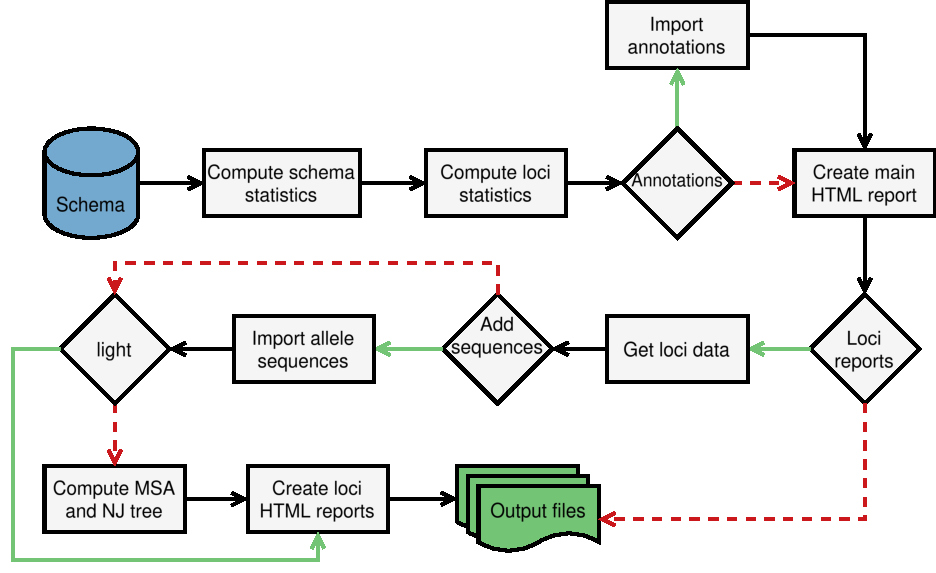
\includegraphics[angle=0,width=\textwidth]{figures/chapter 2/FigureS20.pdf}
    \caption{Diagram of the SchemaEvaluator module. The SchemaEvaluator module analyses a schema to create a report that allows users to explore schema structure and loci diversity interactively. The process starts by computing schema statistics, such as the number of loci and alleles, and loci statistics, such as the number of alleles, allele size statistics, and the number of valid and invalid alleles (e.g. alleles that cannot be translated due to being incomplete, containing ambiguous bases, in-frame stop codons, etc.). The schema and loci statistics are included in interactive data tables and charts on the main page of the HTML report. Loci annotations are imported and included in the main page of the report if provided. If the --loci-reports option is provided, the process performs a detailed analysis of each locus to add a separate locus page to the HTML report for each locus. Loci data is analyzed in greater detail to get more detailed statistics per locus. If the --add-sequences option is provided, the allele DNA sequences are imported and translated to add DNA and protein sequences to code editors on the locus page, which facilitates identifying and manipulating alleles of interest. Additionally, the process computes a multiple sequence alignment (MSA) for each locus at the protein level with MAFFT to display the MSA and MAFFT's guide tree on interactive components. The MSA and guide tree are not displayed if the --light option is provided. The green document icons represent output files. Grey rectangle icons represent analysis steps. Diamond icons represent conditional statements, with green arrows used when the condition is met and red dashed arrows otherwise. The blue cylinder icon represents a schema.}
    \label{fig:chap2_figureS20}
\end{figure*}

\newpage
\begin{figure*}[h!]
    \centering
    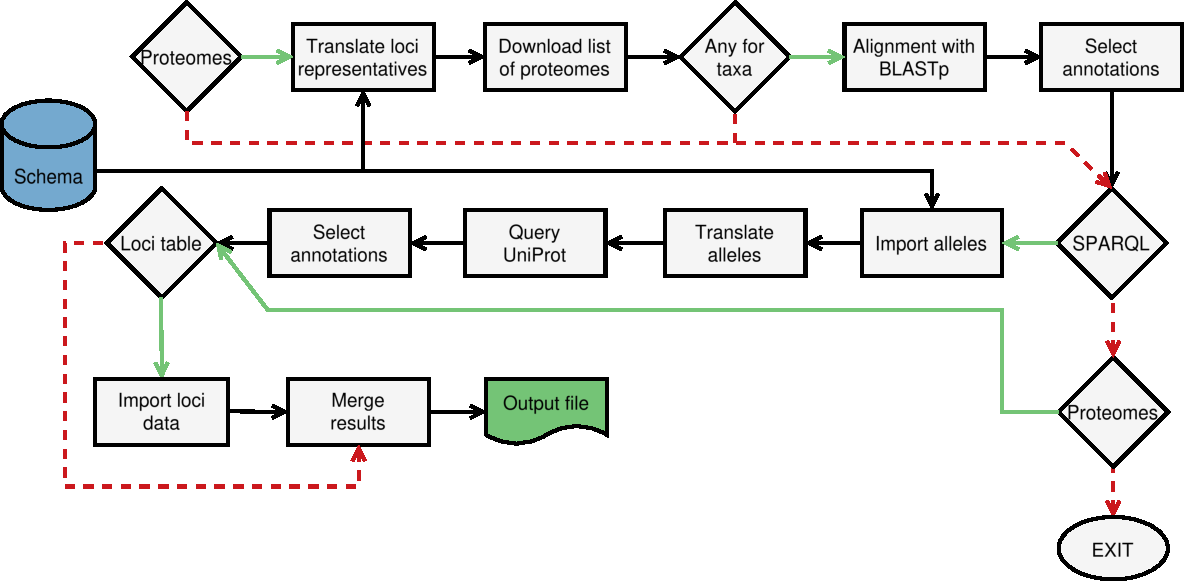
\includegraphics[angle=0,width=\textwidth]{figures/chapter 2/FigureS21.pdf}
    \caption{Diagram of the UniprotFinder module. The UniprotFinder module determines annotations for schema loci. The module offers two options to determine annotations: aligning against UniProt's reference proteomes and exact matching through UniProt's SPARQL endpoint. Users must provide at least one valid taxon name to annotate based on the reference proteomes. The process downloads the list of reference proteomes and searches for proteomes for the specified taxa. If there are any proteomes for the specified taxa, they are downloaded, and the loci representative alleles are aligned against the reference proteomes so annotations can be selected based on the BSR. The process searches for annotations through UniProt's SPARQL endpoint by creating queries including the loci alleles and submitting requests to the endpoint. If an allele matches any protein in UniProt, the annotation terms are extracted from the results. The process tries to select the most informative annotation terms. The annotation terms found through both options are merged to create a single annotations table. If the user provides a TSV file with additional loci data, such as the file with CDS coordinates created by the CreateSchema and AlleleCall modules, the process will add the data in that file to the annotations table. The green document icon represents the output file. Grey rectangle icons represent analysis steps. Diamond icons represent conditional statements, with green arrows used when the condition is met and red dashed arrows otherwise. The blue cylinder icon represents a schema.}
    \label{fig:chap2_figureS21}
\end{figure*}

\newpage
\begin{figure*}[h!]
    \centering
    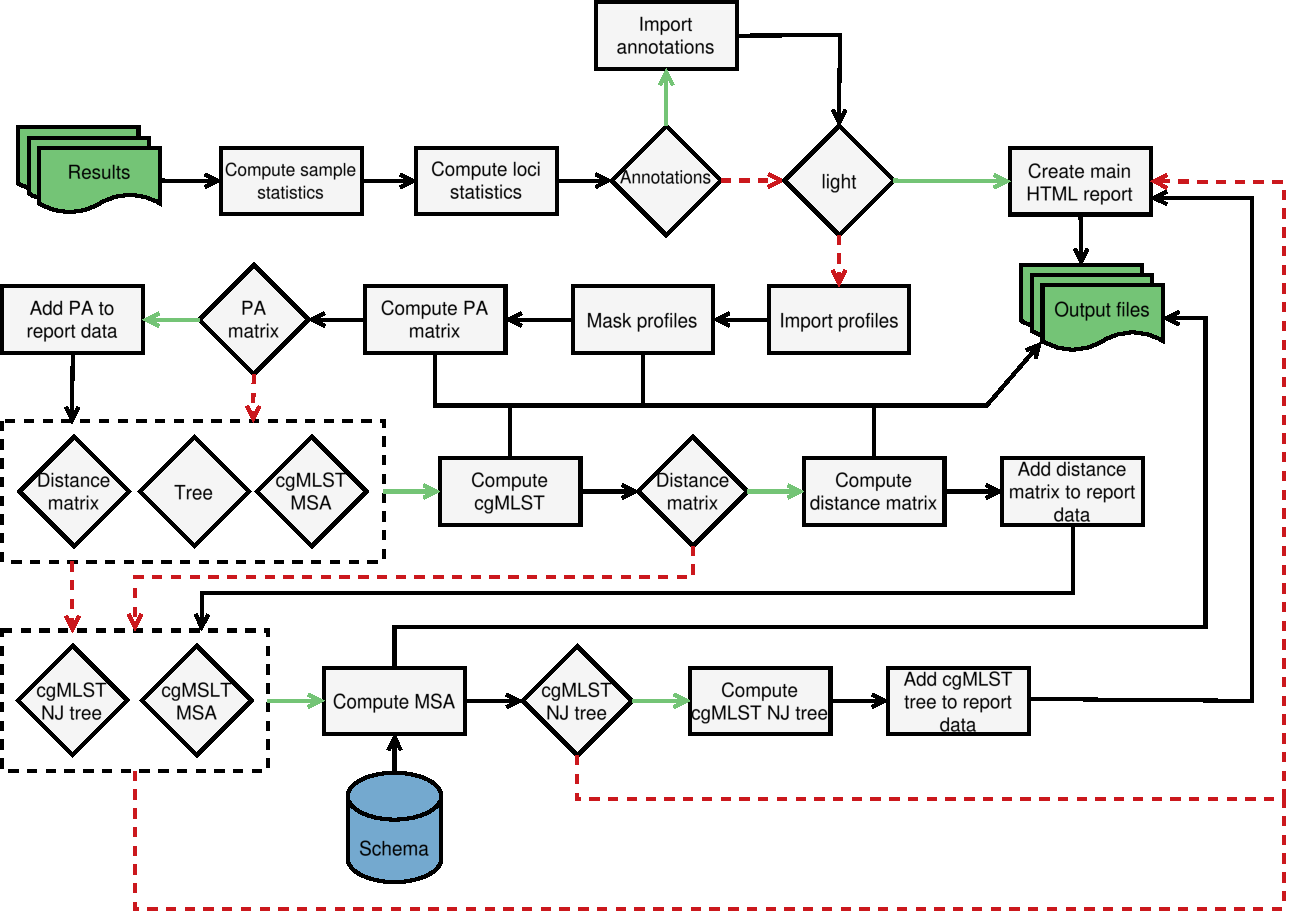
\includegraphics[angle=0,width=\textwidth]{figures/chapter 2/FigureS22.pdf}
    \caption{Diagram of the AlleleCallEvaluator module. The AlleleCallEvaluator module analyses allele calling results to create a report that allows users to explore results interactively. The process starts by importing and computing sample and loci statistics based on the allele calling results. The sample and loci statistics are included in interactive data tables and charts on the main page of the HTML report. Loci annotations are imported and included in the main page of the report if provided. If the --light option is provided, the process does not add more information to the report. Otherwise, the allelic profiles are imported and masked to remove INF- prefixes and substitute special classifications by 0. The masked profiles serve as the basis for computing a presence-absence (PA) matrix, enabling the determination of the set of loci that constitute the core genome. The profile data for the core loci are used to compute a matrix of allelic distances. The core loci alleles identified per strain and locus are imported to compute the cgMLST alignment that FastTree uses to compute a Neighbour-Joining (NJ) tree. The PA and distance matrices and NJ tree data are included in the report to be displayed and explored interactively. The green document icons represent input and output files. Grey rectangle icons represent analysis steps. Diamond icons represent conditional statements, with green arrows used when the condition is met and red dashed arrows otherwise. The blue cylinder icon represents a schema.}
    \label{fig:chap2_figureS22}
\end{figure*}

\newpage
\begin{landscape}
\vspace*{\fill}
\begin{table}[h!]
\caption{Supplementary table 1.}
\label{tab:ch2_suptable1}
\resizebox{\linewidth}{!}{%
\begin{tabular}{ll}
\toprule
\multicolumn{2}{c}{\textbf{FastQ Toolkit v2.2.0}}                                       \\ \midrule
Minimum read length                             & 32                           \\
Sub-sampling                                    & FALSE                        \\
Adapter trim stringency                         & 0.9                          \\
Select respective adapters                      & TRUE                         \\
Quality trimming                                & FALSE                        \\
Poly-A/T Trimming                               & FALSE                        \\
Read Filtering                                  & FALSE                        \\
Modify Reads                                    & FALSE                        \\
Fix Format                                      & FALSE                        \\ \midrule
\multicolumn{2}{c}{\textbf{FastQC v1.0.0}}                                              \\ \midrule
Kmer Size                                       & 5                            \\
Use Conatminant Filter                          & TRUE                         \\ \midrule
\multicolumn{2}{c}{\textbf{Kraken Metagenomics v1.0.0}}                                 \\ \midrule
Host Filter                                     & TRUE RefSeqhg19              \\
Classification Database                         & MiniKraken 20141208 (latest) \\
Filter Threshold                                & 0                            \\ \midrule
\multicolumn{2}{c}{\textbf{Metaphlan v1.0.0}}                                           \\ \midrule
Sensitivity options for read-marker similarity (as descibed by BowTie2)                  & Very Sensitive \\
\multicolumn{2}{c}{\textbf{SPAdes Genome Assembler v3.9.0}}                             \\
Running Mode                                    & Error Correction \& Assembly \\
Dataset type                                    & Multi Cell                   \\
Careful Mode                                    & Disable                      \\
k-mer lengths                                   & Auto                         \\ \midrule
\multicolumn{2}{c}{\textbf{SEAR: Antibiotic Resistance v1.0.0}}                                           \\ \midrule
Read length cutoff (bases)                      & 70                           \\
Read quality score cutoff                       & 20                           \\
Read subtraction against E.coli reference genome (K12)?                                  & No             \\
Clustering stringency (express \% as a decimal) & 0.98                         \\
Annotation stringency (\% length of reference ARG sequence mapped to by sequencing reads & 40             \\\midrule
\multicolumn{2}{c}{\textbf{GENIUS Metagenomics: Know Now v1.1.0}}                                                  \\ \midrule
Can't set any settings in BaseSpace             & \\                    \midrule    
\end{tabular}%
}
\end{table}
\vspace*{\fill}
\end{landscape}

\newpage
\begin{landscape}
\vspace*{\fill}
\begin{table}[h!]
\caption{Supplementary table 2.}
\label{tab:ch2_suptable2}
\resizebox{\linewidth}{!}{%
\begin{tabular}{ll}
\midrule
\multicolumn{2}{c}{\textbf{Trim Reads}}                                                          \\\midrule
Trimmomatic v0.36 (INNUca v2.6 initial module)     &                                    \\
Quality trim                                       & TRUE                               \\
Phred Quality limit                                & 05:20                              \\
Trim adapter list                                  & Illumina adapters                  \\
Remove 5' terminal nucleotides                     & TRUE                               \\
Number of 5' terminal nucleotides                  & 3                                  \\
Remove 3' terminal nucleotides                     & TRUE                               \\
Number of 3' terminal nucleotides                  & 3                                  \\
Discard short reads                                & TRUE                               \\
Minimum number of nucleotides in reads             & 55 \\              
\midrule
\multicolumn{2}{c}{\textbf{Map Reads to Reference}}                                              \\\midrule
Bowtie2 v2.3.2                                     &                                    \\
References                                         & Homo sapiens (hg19) index          \\
Mode                                               & end-to-end                         \\
Mode option                                        & sensitive                          \\
Collect unmapped reads                             & FALSE                              \\
\midrule
\multicolumn{2}{c}{\textbf{Taxonomic Classification}}                                            \\\midrule
Kraken v0.10.5-beta                                &                                    \\
References                                         & miniKraken database (Dec. 8, 2014) \\
K-mer length                                       & 35                                 \\
MIDAS                                              &                                    \\
References                                         & midas\_db\_v1.2 (May 9, 2018)      \\
Word size for blast                                & 28                                 \\
Alignment coverage                                 & 0.75                               \\
MetaPhlAn2 v2.0                                    &                                    \\
References                                         & default database (May 9, 2018)     \\
Minimum total nucleotide length for the markers    & 2000                               \\
Quantile value for robust average                  & 0.1                                \\
Statistical approach for converting marker abundances into clade abundances & clade global                                          \\
Analysis type                                                               & profiling a metagenome in terms of relative abundance \\
\midrule
\multicolumn{2}{c}{\textbf{Identify MLST}}                                                       \\\midrule
metaMLST v1.1                                      &                                    \\
References                                         & metamlstDB\_2017                   \\
Bowtie2 mode                                       & local                              \\
Bowtie2 mode option                                & very sensitive local               \\
Collect unmapped reads                             & FALSE                              \\
Search for and report all alignment                & TRUE                               \\
\midrule
\multicolumn{2}{c}{\textbf{Find Resistance Genes}}                                               \\\midrule
ReMatCh v3.2                                       &                                    \\
References                                         & ResFinder database (29-06-2017)    \\
Minimum coverage to consider a position as present & 1                                  \\
Minimum coverage depth to perform a basecall       & 1                                  \\
Minimum gene coverage (\%)                         & 80                                 \\
Minimum gene identity (\%)                         & 70                                 \\
\midrule
\multicolumn{2}{c}{\textbf{\textit{De Novo} Assembly}}                                                    \\\midrule
SPAdes v3.10.1                                     &                                    \\
Mode                                               & careful                            \\
Error correction                                   & FALSE                              \\
Read coverage cut-off value                        & 2                                  \\
List of K-mers                                     & 21,33,55,67,77                     \\
\midrule
\multicolumn{2}{c}{\textbf{Plasmid Detection}}                                                   \\\midrule
Bowtie2 v2.3.2                                     &                                    \\
References                                         & NCBI RefSeq (May 11, 2017)         \\
Mode                                               & end-to-end                         \\
Mode option                                        & sensitive                          \\
Collect unmapped reads                             & FALSE                              \\
Multiple alignment                                 & TRUE \\
\midrule
\end{tabular}%
}
\end{table}
\vspace*{\fill}
\end{landscape}

\newpage
\begin{landscape}
\vspace*{\fill}
\begin{table}[h!]
    \caption[Runtime (in minutes, min) and peak memory usage (in megabytes, MB) for the adaptation of the schemas downloaded from cgMLST.org with chewBBACA 2 and chewBBACA 3.]{Runtime (in minutes, min) and peak memory usage (in megabytes, \ac{MB}) for the adaptation of the schemas downloaded from cgMLST.org with chewBBACA 2 and chewBBACA 3.}
    \label{tab:ch2_tableS3}
    \centering
    \begin{tabular}{@{}lllll@{}}
    \toprule
    \multicolumn{1}{|c|}{} & \multicolumn{2}{|c|}{Runtime (min)} & \multicolumn{2}{|c|}{Memory (MB)} \\ \midrule
    Species & chewBBACA 2 & chewBBACA 3 & chewBBACA 2 & chewBBACA 3 \\ \midrule
    \textit{S. pyogenes} & 630.94 & 0.47 & 91.39 & 128.58 \\
    \textit{L. monocytogenes} & 6218.59 & 2.07 & 92.05 & 143.55 \\
    \textit{S. enterica} & 17428.95 & 4.51 & 93.44 & 147.23 \\
    \bottomrule
    \end{tabular}
\end{table}
\vspace*{\fill}
\end{landscape}

\newpage
\begin{landscape}
\vspace*{\fill}
\begin{table}[h!]
    \caption{Number of loci in the schemas download from cgMLST.org, number of loci in the adapted schemas, and number of loci whose diversity is not completly captured by the selected representative alleles.}
    \label{tab:ch2_tableS4}
    \centering
    \resizebox{\linewidth}{!}{
    \small
    \begin{tabular}{@{}llllll@{}}
    \toprule
    \multicolumn{2}{|c|}{} & \multicolumn{2}{|c|}{Adapted loci} & \multicolumn{2}{|c|}{Loci not totally covered by selected representative alleles} \\ \midrule
    Species & Number of loci in original schema (cgMLST.org) & chewBBACA 2 & chewBBACA 3 & chewBBACA 2 & chewBBACA 3 \\ \midrule
    \textit{S. pyogenes} & 1095 & 1095 & 1095 & 1 & 0 \\
    \textit{L. monocytogenes} & 1701 & 1701 & 1701 & 15 & 0 \\
    \textit{S. enterica} & 3002 & 2999 & 2999 & 64 & 0 \\
    \bottomrule
    \end{tabular}
    }
\end{table}
\vspace*{\fill}
\end{landscape}

\newpage
\begin{landscape}
\vspace*{\fill}
\begin{table}[h!]
    \caption{Number of loci in the wgMLST and cgMLST schemas, and number of alleles in the cgMLST schemas after performing allele calling with each tool with the complete genomes.}
    \label{tab:ch2_tableS5}
    \centering
    \begin{tabular}{@{}llllll@{}}
    \toprule
    \multicolumn{1}{|c|}{} & \multicolumn{2}{|c|}{Number of loci} & \multicolumn{3}{|c|}{Number of alleles in cgMLST} \\ \midrule
    Species & wgMLST & cgMLST & chewBBACA 3 & chewBBACA 2 & pyMLST \\ \midrule
    \textit{S. pyogenes} & 3688 & 1345 & 71092 & 71092 & 60292 \\
    \textit{L. monocytogenes} & 5760 & 2449 & 87376 & 87376 & 52477 \\
    \textit{S. enterica} & 23373 & 3192 & 341247 & 341247 & 251502 \\
    \bottomrule
    \end{tabular}
\end{table}
\vspace*{\fill}
\end{landscape}

\newpage
\begin{landscape}
\vspace*{\fill}
\begin{table}[h!]
    \caption[Mean runtime values in minutes for the allele calling of each species' datasets with chewBBACA 3, chewBBACA 2 and pyMLST.]{Mean runtime values in minutes for the allele calling of each species' datasets with chewBBACA 3, chewBBACA 2 and pyMLST.}
    \label{tab:ch2_tableS6}
    \centering
    \resizebox{\linewidth}{!}{
    \begin{tabular}{@{}llllllllll@{}}
    \toprule
    \multicolumn{1}{|c|}{} & \multicolumn{3}{|c|}{\textit{S. pyogenes}} & \multicolumn{3}{|c|}{\textit{L. monocytogenes}} & \multicolumn{3}{|c|}{\textit{S. enterica}} \\ \midrule
    Dataset size & chewBBACA 3 & chewBBACA 2 & pyMLST & chewBBACA 3 & chewBBACA 2 & pyMLST & chewBBACA 3 & chewBBACA 2 & pyMLST \\ \midrule
    1 & 0.10 & 0.19 & 0.17 & 0.16 & 0.37 & 0.20 & 0.29 & 0.57 & 0.51 \\
    2 & 0.12 & 0.23 & 0.32 & 0.20 & 0.48 & 0.42 & 0.33 & 0.62 & 1.23 \\
    4 & 0.14 & 0.27 & 0.61 & 0.26 & 0.62 & 0.84 & 0.50 & 1.32 & 2.11 \\
    8 & 0.22 & 0.48 & 1.24 & 0.36 & 0.94 & 1.72 & 0.80 & 2.14 & 3.90 \\
    16 & 0.26 & 0.65 & 2.46 & 0.56 & 1.78 & 3.51 & 1.07 & 3.28 & 7.21 \\
    32 & 0.40 & 1.30 & 4.93 & 0.73 & 2.77 & 6.89 & 1.58 & 5.32 & 14.18 \\
    64 & 0.59 & 2.37 & 9.86 & 1.03 & 4.75 & 13.73 & 2.60 & 11.17 & 28.47 \\
    128 & 0.87 & 4.68 & 20.13 & 1.64 & 9.96 & 27.39 & 3.88 & 20.34 & 56.03 \\
    256 & 1.38 & 8.52 & 41.05 & 2.59 & 19.69 & 54.74 & 6.16 & 41.01 & 111.64 \\
    512 & 2.20 & 16.36 & 82.09 & 4.18 & 36.14 & 109.26 & 9.73 & 77.05 & 222.02 \\
    1024 & 3.71 & 29.11 & 163.95 & 7.18 & 69.58 & 218.93 & 16.51 & 146.31 & 445.61 \\
    2048 & 6.67 & 52.25 & 329.27 & 12.97 & 134.03 & 439.27 & 29.37 & 276.28 & 891.29 \\
    4096 & 12.77 & 94.81 & 663.53 & 25.29 & 255.43 & 879.07 & 56.69 & 527.09 & 1786.59 \\
    8192 & 26.26 & 175.87 & 1339.27 & 54.45 & 501.13 & 1762.43 & 109.52 & 1463.99 & 3578.79 \\
    16384 & 60.63 & 342.76 & 2680.91 & 115.65 & 2347.44 & 3531.93 & 216.80 & 4227.74 & 7171.94 \\
    \bottomrule
    \end{tabular}
    }
\end{table}
\vspace*{\fill}
\end{landscape}

\newpage
\begin{landscape}
\vspace*{\fill}
\begin{table}[h!]
    \caption{Mean values for the total number of coding sequences (CDSs), distinct number of CDSs, and percentage of total CDSs that are distinct for each species' datasets.}
    \label{tab:ch2_tableS7}
    \centering
    \resizebox{\linewidth}{!}{
    \begin{tabular}{@{}llllllllll@{}}
    \toprule
    \multicolumn{1}{|c|}{} & \multicolumn{3}{|c|}{\textit{S. pyogenes}} & \multicolumn{3}{|c|}{\textit{L. monocytogenes}} & \multicolumn{3}{|c|}{\textit{S. enterica}} \\ \midrule
    Dataset size & Total CDSs & Distinct CDSs & Distinct CDSs (\%) & Total CDSs & Distinct CDSs & Distinct CDSs (\%) & Total CDSs & Distinct CDSs & Distinct CDSs (\%) \\ \midrule
    1 & 1684.8 & 1683.8 & 99.9 & 2966.2 & 2900.4 & 97.8 & 4651.8 & 4593.8 & 98.8 \\
    2 & 3487.8 & 3332.8 & 95.6 & 6037.8 & 5381.4 & 89.2 & 9141 & 8745.2 & 95.7 \\
    4 & 6909.8 & 5667.4 & 82.2 & 12211.2 & 9292.4 & 76.1 & 18188.8 & 15520.6 & 85.4 \\
    8 & 13915.6 & 10406.8 & 74.9 & 24325 & 15508.8 & 63.8 & 36792.2 & 28367.2 & 77.2 \\
    16 & 27815.4 & 14623.2 & 52.6 & 48774.6 & 22782 & 46.7 & 73943.6 & 45437.8 & 61.5 \\
    32 & 55772.8 & 22583 & 40.5 & 97534.4 & 32150.6 & 33.0 & 147210.6 & 74236.6 & 50.4 \\
    64 & 111138.4 & 37902.4 & 34.1 & 194415.6 & 42912.2 & 22.1 & 295221.8 & 121113.2 & 41.0 \\
    128 & 221802.8 & 51898.4 & 23.4 & 388199.4 & 63592.6 & 16.4 & 589450.4 & 183784.6 & 31.2 \\
    256 & 443839.8 & 75020 & 16.9 & 778822.6 & 91800.6 & 11.8 & 1179475.4 & 269535.4 & 22.9 \\
    512 & 890029.2 & 106781.6 & 12.0 & 1556165.4 & 127843.8 & 8.2 & 2357310.8 & 383924.2 & 16.3 \\
    1024 & 1777989.2 & 146328.4 & 8.2 & 3109809.6 & 188643 & 6.1 & 4707795.8 & 540833 & 11.5 \\
    2048 & 3557437.8 & 197893.8 & 5.6 & 6222051.4 & 280055.4 & 4.5 & 9428540.8 & 759312.4 & 8.1 \\
    4096 & 7113644 & 261355.4 & 3.7 & 12447727 & 404021.6 & 3.3 & 18853371.4 & 1068649.6 & 5.7 \\
    8192 & 14226635.6 & 339833.2 & 2.4 & 24891444.2 & 585723.2 & 2.4 & 37705899 & 1529198.2 & 4.1 \\
    16394 & 28451923 & 430352 & 1.5 & 49787476 & 861124 & 1.7 & 75417045 & 2118041 & 2.8 \\
    \bottomrule
    \end{tabular}
    }
\end{table}
\vspace*{\fill}
\end{landscape}

\newpage
\begin{landscape}
\vspace*{\fill}
\begin{table}[h!]
    \caption[Mean peak memory usage values in megabytes for the allele calling of each species' datasets with chewBBACA 3, chewBBACA 2 and pyMLST.]{Mean peak memory usage values in megabytes for the allele calling of each species' datasets with chewBBACA 3, chewBBACA 2 and pyMLST.}
    \label{tab:ch2_tableS8}
    \centering
    \resizebox{\linewidth}{!}{
    \begin{tabular}{@{}llllllllll@{}}
    \toprule
    \multicolumn{1}{|c|}{} & \multicolumn{3}{|c|}{\textit{S. pyogenes}} & \multicolumn{3}{|c|}{\textit{L. monocytogenes}} & \multicolumn{3}{|c|}{\textit{S. enterica}} \\ \midrule
    Dataset size & chewBBACA 3 & chewBBACA 2 & pyMLST & chewBBACA 3 & chewBBACA 2 & pyMLST & chewBBACA 3 & chewBBACA 2 & pyMLST \\ \midrule
    1 & 245.59 & 74.80 & 80.46 & 300.35 & 76.85 & 84.23 & 383.88 & 78.50 & 88.33 \\
    2 & 285.55 & 75.23 & 80.35 & 331.48 & 78.72 & 84.79 & 451.37 & 80.15 & 88.30 \\
    4 & 348.74 & 76.72 & 80.72 & 459.23 & 81.35 & 84.68 & 617.49 & 85.02 & 89.76 \\
    8 & 444.45 & 79.88 & 81.55 & 616.80 & 88.08 & 85.73 & 784.73 & 91.39 & 90.00 \\
    16 & 463.58 & 89.36 & 81.96 & 629.87 & 101.95 & 86.06 & 871.55 & 107.73 & 93.26 \\
    32 & 466.22 & 105.75 & 84.22 & 672.21 & 120.75 & 87.45 & 915.02 & 142.70 & 95.91 \\
    64 & 564.50 & 142.06 & 84.49 & 736.91 & 157.54 & 91.82 & 1029.75 & 197.62 & 96.56 \\
    128 & 649.79 & 163.51 & 86.14 & 794.65 & 209.10 & 93.04 & 1134.74 & 250.34 & 101.99 \\
    256 & 700.47 & 237.88 & 86.41 & 830.57 & 325.06 & 93.25 & 1290.67 & 422.44 & 104.91 \\
    512 & 789.30 & 380.45 & 86.38 & 888.29 & 567.43 & 94.21 & 1424.32 & 737.53 & 104.92 \\
    1024 & 865.61 & 691.73 & 86.74 & 974.11 & 1073.47 & 93.98 & 1609.24 & 1424.54 & 105.26 \\
    2048 & 970.07 & 1301.39 & 86.77 & 1084.84 & 2069.30 & 94.28 & 1948.72 & 2767.81 & 105.94 \\
    4096 & 1076.68 & 2517.72 & 87.01 & 1300.98 & 4000.32 & 94.52 & 2327.89 & 5376.79 & 105.42 \\
    8192 & 1237.61 & 4931.30 & 86.98 & 1575.37 & 7913.11 & 94.51 & 3108.47 & 10671.73 & 105.98 \\
    16384 & 1538.04 & 9792.28 & 87.39 & 2287.09 & 15749.59 & 94.20 & 4235.34 & 21251.72 & 106.15 \\
    \bottomrule
    \end{tabular}
    }
\end{table}
\vspace*{\fill}
\end{landscape}

\newpage
\begin{landscape}
\vspace*{\fill}
\begin{table}[h!]
    \caption[Mean runtime values in minutes for the allele calling of each species' datasets with chewBBACA 3's four execution modes.]{Mean runtime values in minutes for the allele calling of each species' datasets with chewBBACA 3's four execution modes.}
    \label{tab:ch2_tableS9}
    \centering
    \resizebox{\linewidth}{!}{
    \begin{tabular}{@{}lllllllllllll@{}}
    \toprule
    \multicolumn{1}{|c|}{} & \multicolumn{4}{|c|}{\textit{S. pyogenes}} & \multicolumn{4}{|c|}{\textit{L. monocytogenes}} & \multicolumn{4}{|c|}{\textit{S. enterica}} \\ \midrule
    Dataset size & Mode 1 & Mode 2 & Mode 3 & Mode 4 & Mode 1 & Mode 2 & Mode 3 & Mode 4 & Mode 1 & Mode 2 & Mode 3 & Mode 4 \\ \midrule
    1 & 0.04 & 0.05 & 0.08 & 0.10 & 0.07 & 0.08 & 0.13 & 0.16 & 0.13 & 0.14 & 0.21 & 0.28 \\
    2 & 0.04 & 0.06 & 0.10 & 0.12 & 0.07 & 0.08 & 0.15 & 0.20 & 0.13 & 0.15 & 0.22 & 0.33 \\
    4 & 0.05 & 0.06 & 0.12 & 0.14 & 0.07 & 0.09 & 0.19 & 0.26 & 0.14 & 0.19 & 0.33 & 0.51 \\
    8 & 0.06 & 0.08 & 0.17 & 0.22 & 0.09 & 0.12 & 0.26 & 0.37 & 0.17 & 0.24 & 0.52 & 0.82 \\
    16 & 0.08 & 0.10 & 0.20 & 0.26 & 0.12 & 0.16 & 0.39 & 0.56 & 0.23 & 0.33 & 0.62 & 1.07 \\
    32 & 0.12 & 0.16 & 0.33 & 0.42 & 0.18 & 0.24 & 0.49 & 0.74 & 0.42 & 0.47 & 0.87 & 1.58 \\
    64 & 0.19 & 0.25 & 0.47 & 0.61 & 0.31 & 0.38 & 0.71 & 1.03 & 0.65 & 0.84 & 1.42 & 2.60 \\
    128 & 0.32 & 0.41 & 0.71 & 0.88 & 0.56 & 0.69 & 1.13 & 1.65 & 1.05 & 1.31 & 2.01 & 3.88 \\
    256 & 0.63 & 0.74 & 1.08 & 1.35 & 1.08 & 1.25 & 1.78 & 2.58 & 2.10 & 2.48 & 3.34 & 6.11 \\
    512 & 1.19 & 1.35 & 1.81 & 2.21 & 2.03 & 2.26 & 2.93 & 4.17 & 3.87 & 4.52 & 5.54 & 9.74 \\
    1024 & 2.33 & 2.63 & 3.21 & 3.79 & 4.18 & 4.60 & 5.45 & 7.22 & 7.67 & 8.62 & 9.99 & 16.43 \\
    2048 & 4.70 & 5.12 & 5.86 & 6.69 & 8.45 & 9.13 & 10.32 & 12.98 & 16.21 & 17.89 & 19.71 & 29.40 \\
    4096 & 9.84 & 10.52 & 11.55 & 12.77 & 18.41 & 19.70 & 21.39 & 25.44 & 36.97 & 39.53 & 41.94 & 56.25 \\
    8192 & 22.14 & 23.32 & 24.81 & 26.69 & 43.50 & 45.82 & 48.56 & 54.71 & 78.66 & 81.90 & 86.39 & 109.49 \\
    16384 & 54.21 & 56.25 & 58.64 & 61.20 & 98.39 & 101.03 & 105.28 & 115.84 & 172.90 & 175.64 & 182.55 & 220.60 \\
    \bottomrule
    \end{tabular}
    }
\end{table}
\vspace*{\fill}
\end{landscape}

\newpage
\begin{landscape}
\vspace*{\fill}
\begin{table}[h!]
    \caption{Mean peak memory usage values in megabytes for the allele calling of each species' datasets with chewBBACA 3's four execution modes.}
    \label{tab:ch2_tableS10}
    \centering
    \resizebox{\linewidth}{!}{
    \begin{tabular}{@{}lllllllllllll@{}}
    \toprule
    \multicolumn{1}{|c|}{} & \multicolumn{4}{|c|}{\textit{S. pyogenes}} & \multicolumn{4}{|c|}{\textit{L. monocytogenes}} & \multicolumn{4}{|c|}{\textit{S. enterica}} \\ \midrule
    Dataset size & Mode 1 & Mode 2 & Mode 3 & Mode 4 & Mode 1 & Mode 2 & Mode 3 & Mode 4 & Mode 1 & Mode 2 & Mode 3 & Mode 4 \\ \midrule
    1 & 207.17 & 236.03 & 243.21 & 245.41 & 241.32 & 278.33 & 291.99 & 300.58 & 334.90 & 356.94 & 376.05 & 373.74 \\
    2 & 247.25 & 274.51 & 285.88 & 285.58 & 310.95 & 316.36 & 357.78 & 335.50 & 428.30 & 431.12 & 436.29 & 448.07 \\
    4 & 326.66 & 347.68 & 348.49 & 352.61 & 452.29 & 452.32 & 466.07 & 459.63 & 617.17 & 614.39 & 614.29 & 635.11 \\
    8 & 422.72 & 441.80 & 444.70 & 449.01 & 608.20 & 611.59 & 623.93 & 627.72 & 786.50 & 782.67 & 778.62 & 786.11 \\
    16 & 445.85 & 464.16 & 467.19 & 467.81 & 621.31 & 620.10 & 625.42 & 632.11 & 871.49 & 867.79 & 871.27 & 864.63 \\
    32 & 468.18 & 467.03 & 466.80 & 466.77 & 672.06 & 671.52 & 672.82 & 671.89 & 912.87 & 918.69 & 912.17 & 914.32 \\
    64 & 564.73 & 564.28 & 562.36 & 565.82 & 736.79 & 738.39 & 737.35 & 737.71 & 1018.99 & 1013.50 & 1029.77 & 1027.37 \\
    128 & 649.72 & 648.26 & 655.04 & 651.98 & 794.47 & 795.35 & 794.25 & 795.16 & 1151.16 & 1178.55 & 1150.94 & 1158.56 \\
    256 & 706.43 & 704.90 & 700.72 & 706.41 & 831.13 & 831.47 & 835.84 & 837 & 1251.01 & 1277.62 & 1261.15 & 1281.28 \\
    512 & 787.97 & 801.64 & 792.56 & 789.06 & 882.62 & 882.87 & 889.19 & 888.90 & 1436.54 & 1392.310156 & 1383.53 & 1428.23 \\
    1024 & 866.24 & 866.88 & 868.71 & 866.87 & 969.94 & 982.68 & 969.36 & 976.03 & 1583.510156 & 1628.719531 & 1619.13 & 1620.02 \\
    2048 & 970.48 & 970.21 & 970.40 & 970.10 & 1085.65 & 1059.37 & 1071.66 & 1077.11 & 1969.12 & 1915.98 & 1950.73 & 1945.92 \\
    4096 & 1077.019531 & 1076.55 & 1076.57 & 1076.98 & 1252.169531 & 1274.26 & 1283.17 & 1316.99 & 2258.61 & 2163.53 & 2170.379688 & 2251.50 \\
    8192 & 1236.29 & 1244.03 & 1242.92 & 1246.09 & 1455.23 & 1473.02 & 1538.639844 & 1608.01 & 2962.67 & 3009.10 & 3110.929688 & 3100.90 \\
    16384 & 1537.65 & 1536.51 & 1538.26 & 1540.00 & 2110.769531 & 2096.86 & 2249.089844 & 2232.05 & 3958.66 & 3963.51 & 4222.44 & 4232.04 \\
    \bottomrule
    \end{tabular}
    }
\end{table}
\vspace*{\fill}
\end{landscape}

\newpage
\begin{landscape}
\vspace*{\fill}
\begin{table}[h!]
    \caption{Number of loci in each species' cgMLST schemas, number of core and accessory loci determined based on each tool's results and number of core and accessory loci determined based on chewBBACA 2's and pyMLST's results that are shared with the sets of core and accessory loci determined based on chewBBACA 3's results.}
    \label{tab:ch2_tableS11}
    \centering
    \resizebox{\linewidth}{!}{
    \begin{tabular}{@{}llllllllllll@{}}
    \toprule
    \multicolumn{2}{|c|}{} & \multicolumn{3}{|c|}{core loci} & \multicolumn{3}{|c|}{accessory loci} & \multicolumn{2}{|c|}{core loci shared with chewBBACA 3} & \multicolumn{2}{|c|}{accessory loci shared with chewBBACA 3} \\ \midrule
    Species & Schema loci & chewBBACA 2 & chewBBACA 3 & pyMLST & chewBBACA 2 & chewBBACA 3 & pyMLST & chewBBACA 2 & pyMLST & chewBBACA 2 & pyMLST \\ \midrule
    S. pyogenes & 1345 & 1322 & 1321 & 1075 & 23 & 24 & 270 & 1321 & 1073 & 23 & 22 \\
    L. monocytogenes & 2449 & 2313 & 2314 & 1022 & 136 & 135 & 1427 & 2312 & 983 & 134 & 96 \\
    S. enterica & 3192 & 3001 & 3009 & 2365 & 191 & 183 & 827 & 3000 & 2255 & 182 & 72 \\
    \bottomrule
    \end{tabular}
    }
\end{table}
\vspace*{\fill}
\end{landscape}

\newpage
\begin{landscape}
\vspace*{\fill}
\begin{table}[h!]
    \caption[Total number of coding sequences (CDSs) predicted by Pyrodigal for each species' complete dataset, total number of CDSs classified by each tool, percentage of the total CDSs classified by each tool and average number of CDSs classified per strain.]{Total number of coding sequences (\acp{CDS}) predicted by Pyrodigal for each species' complete dataset, total number of \acp{CDS} classified by each tool, percentage of the total \acp{CDS} classified by each tool and average number of \acp{CDS} classified per strain.}
    \label{tab:ch2_tableS12}
    \centering
    \resizebox{\linewidth}{!}{
    \begin{tabular}{@{}lllllllllll@{}}
    \toprule
    \multicolumn{2}{|c|}{} & \multicolumn{3}{|c|}{Total CDSs classified} & \multicolumn{3}{|c|}{Percentage of total CDSs classified} & \multicolumn{3}{|c|}{Average number of CDSs classified per strain} \\ \midrule
    Species & Total number of CDSs (n=16384) & chewBBACA 3 & chewBBACA 2 & pyMLST & chewBBACA 3 & chewBBACA 2 & pyMLST & chewBBACA 3 & chewBBACA 2 & pyMLST \\ \midrule
    S. pyogenes & 28,451,923 & 21,982,083 & 21,980,537 & 19,092,545 & 77.26 & 77.26 & 67.10 & 1,341.68 & 1,341.59 & 1,165.32 \\
    L. monocytogenes & 49,787,476 & 41,011,719 & 40,100,999 & 23,454,353 & 82.37 & 80.54 & 47.11 & 2,503.16 & 2,447.57 & 1,431.54 \\
    S. enterica & 75,417,045 & 52,680,767 & 52,142,713 & 39,868,671 & 69.85 & 69.14 & 52.86 & 3,215.38 & 3,182.54 & 2,433.39 \\
    \bottomrule
    \end{tabular}
    }
\end{table}
\vspace*{\fill}
\end{landscape}

\newpage
\begin{landscape}
\vspace*{\fill}
\begin{table}[h!]
    \caption{Special classification counts for each species' complete dataset per tool.}
    \label{tab:ch2_tableS13}
    \centering
    \resizebox{\linewidth}{!}{
    \begin{tabular}{@{}lllllllllllllllllll@{}}
    \toprule
    \multicolumn{1}{|c|}{} & \multicolumn{10}{|c|}{chewBBACA 3} & \multicolumn{6}{|c|}{chewBBACA 2} & \multicolumn{2}{|c|}{pyMLST} \\ \midrule
    Species & EXC & INF & PLOT3 & PLOT5 & LOTSC & NIPH & NIPHEM & ALM & ASM & PAMA & EXC & INF & PLOT & NIPH & ALM & ASM & EXC & NIPHEM \\
    S. pyogenes & 21735280 & 218736 & 221 & 1817 & 98 & 154 & 1757 & 1170 & 20841 & 0 & 21736576 & 218665 & 2370 & 504 & 1210 & 20994 & 19078994 & 31 \\
    L. monocytogenes & 38543696 & 538769 & 78 & 5594 & 59 & 23357 & 918118 & 690 & 21541 & 0 & 38552279 & 538435 & 6349 & 932267 & 1149 & 21611 & 23342559 & 289 \\
    S. enterica & 50639542 & 919227 & 308 & 5770 & 31 & 14416 & 523022 & 1309 & 37156 & 31 & 50663361 & 916359 & 6806 & 517896 & 1437 & 36854 & 39838200 & 1200 \\
    \bottomrule
    \end{tabular}
    }
\end{table}
\vspace*{\fill}
\end{landscape}
